\documentclass[final,12pt]{article}    
%%%%%%%%%%%%%%%%%%%%%%%%%%%%%%%%%%%%%%%%%%%%%%%%%%%%%%%%%%%%%
%
%  include packages
%
\usepackage{times}
\usepackage{ifthen}
\usepackage{graphics}
\usepackage{graphicx}
\usepackage{color}
\usepackage{shadow}
\usepackage{makeidx}
\makeindex
%%%%%%%%%%%%%%%%%%%%%%%%%%%%%%%%%%%%%%%%%%%%%%%%%%%%%%%%%%%%%
%
%  if private=false certain descriptions are excluded using
%  the \ifthenelse expression
%
\newboolean{private}\setboolean{private}{true}
\newboolean{qmmm}\setboolean{qmmm}{true}
%%%%%%%%%%%%%%%%%%%%%%%%%%%%%%%%%%%%%%%%%%%%%%%%%%%%%%%%%%%%%
%
%  define commands
%
\newcommand{\block}[1]{\subsubsection[#1]{\shabox{\bf #1}}}
%
\newcommand{\brules}[1]{
\makebox[1in][l]{Rules:}\parbox[t]{110mm}{#1}\hfill\break\hfill}
%
\newcommand{\bdescr}[1]{
\makebox[1in][l]{Description:}\parbox[t]{110mm}{#1}\hfill\break}
%
%\newcommand{\key}[1]{\hfill\break
%\makebox[1in][l]{Keyword:}\parbox[t]{110mm}{{\bf #1}}\hfill\break}
%
\newcommand{\key}[1]{\hfill\break \makebox[1.5in][l]{\bf #1}\hfill\break}
%
%\newcommand{\vdescr}[1]{
%\makebox[1in][l]{}\parbox[t]{110mm}{#1}\hfill\break}
%
\newcommand{\vdescr}[1]{\makebox[1in][l]{}\parbox[t]{110mm}{#1}\hfill\break}
%
\newcommand{\vformat}[1]{
\makebox[1in][l]{}\parbox[t]{110mm}{\makebox[1in][l]{Type:}\parbox[t]{2.7in}{#1}}
\hfill\break}
%
\newcommand{\vrules}[1]{
\makebox[1in][l]{}\parbox[t]{110mm}{\makebox[1in][l]{Rules:}\parbox[t]{2.7in}{#1}}
\hfill\break}
%
\newcommand{\vdefault}[1]{
\makebox[1in][l]{}\parbox[t]{110mm}
{\makebox[1in][l]{Default:}\parbox[t]{2.7in}{#1}}
\hfill\break}
%
\newcommand{\mbax}[1]{#1}
%============================================================
%%%%%%%%%%%%%%%%%%%%%%%%%%%%%%%%%%%%%%%%%%%%%%%%%%%%%%%%%%%%%
%
% prepare titlepage
%
\title{{\bfseries\Huge 
    \hrulefill\\
    \hrulefill Manual for the \hrulefill\\
    \hrulefill \hrulefill Projector Augmented Wave \hrulefill\\
    \hrulefill Method \hrulefill\\}
    \medskip{\LARGE Version 2.0}\\
%\thanks{Peter~E.~Bl\"ochl, Clausthal University of Technology (2003)}\\   
%\resizebox{!}{9.0cm}{\includegraphics[10mm,15mm][90mm,110mm]{big.eps}}
\resizebox{!}{9.0cm}{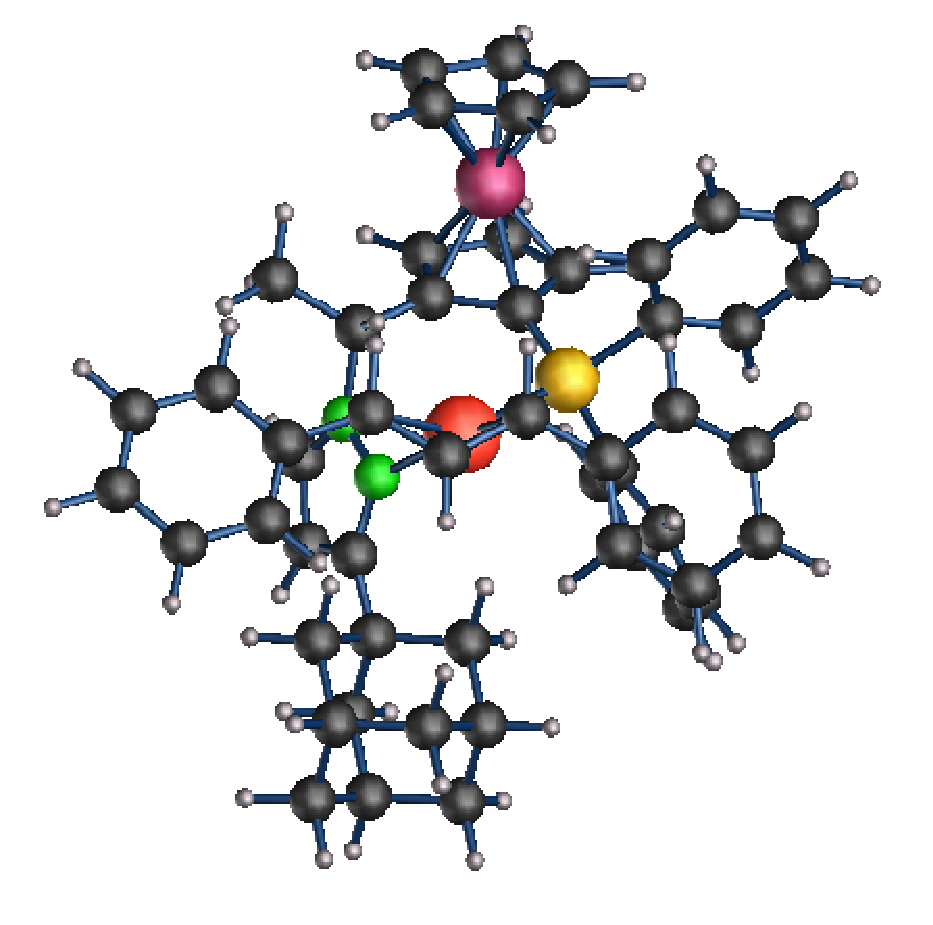
\includegraphics{Figs/big.eps}}
}
\date{\hrulefill\\Peter~E.~Bl\"ochl, Clausthal University of Technology\\(\today)}

\begin{document}          
\maketitle   
%
\noindent            
\setcounter{page}{1}
\footnote{The title picture shows the a chiral Pd complex with P,N ligands,
  a highly enantio-selective catalyst for allylic amination \cite{Pdcat}.}
\newpage
\tableofcontents
%==========================================================================
\newpage
\setcounter{page}{1}
\section{Initial remarks}
%==========================================================================
I am frequently changing the CP-PAW program. Therefore, it is
unavoidable that this description is incomplete in some places,
that it may lists options that are no longer supported, or that it
contains errors. Please let me know if you find something unclear or
even incorrect. Other users will be grateful.

I have attempted to make the program test for inconsistencies of the
input data, such as the selection of conflicting options. You will find
that the program stops in such cases and tries to advise the user
concerning what has gone wrong. New users are particularly creative in
the combinations of options they choose. If you run into problems that
the program does not detect, for example if it crashes without giving
a useful message, please let me know {\em before} you get used to working
around the problem. Your input is particularly valuable in making the
the code more secure to use.

Any other suggestions on how to improve the clarity of this description
or the code are most welcome.

Programs become outdated nearly as quickly as newspapers. Note that
the executable of this code may also have an expiration date.  The
code will print a warning about a month before it expires. Please make
sure that you know the expiration date when you receive an executable.
If the license expires, discuss with your contact person about
obtaining an extension of the license and a new executable program.

Note that the CP-PAW code including all related material is
copyrighted. You require a valid license to execute it. 

%==========================================================================
\section{What is the projector augmented wave method?}
%==========================================================================

The projector augmented wave method \cite{PAW} is an all-electron
electronic structure method, which allows accurate electronic
structure calculations and ab-initio molecular dynamics simulations
on the basis of density functional theory.

What is all that?

{\bf Density functional theory (DFT)} \cite{KohnSham}. Density
functional theory describes the ground state of a many-electron system
by electrons that do not interact other than through an effective
potential that depends on the electron density. It is based on an
exact theorem, which specifies that such a description, based on the
electron density rather than on the electronic many-particle
wave function, be rigorously possible for ground states. In practice the
density functional, which also defines the effective potential as a
functional of the density, is not exactly known. However, highly
successful approximations have been found. In contrast to Hartree-Fock
calculations, density functional theory explicitly treats electron
correlation. The accuracy is typically comparable to that of MP2 calculations,
i.e. only a few kcal/mol \cite{DFTBenchmarks}.

{\bf Ab-initio molecular dynamics (AIMD)} \cite{CP,CP2,Pastore,Madden}
is an extension of traditional electronic structure methods which has
been invented in 1985 by Roberto Car and Michele Parrinello \cite{CP}.
The best way to think of it is as a series of electronic structure
calculations, one for each time slice, for always different atomic
positions. From one time slice to the next, the atomic positions are
changed according to Newton's equations of motion $M_i\ddot R_i=F_i$.
Here $M_i$ is the mass of a nucleus, $R_i$ the position, $F_i$ the
force acting on the nucleus as calculated from the electronic
structure, and the double-dots stand for the second time derivative.
Self-consistent iterations at each time step are avoided by a
dynamical evolution of the wave functions, and thus simulations of
several picoseconds are possible, which is sufficient to simulate
directly chemical reactions and diffusion with low barriers or at high
temperatures.

Whereas the basic idea of ab-initio molecular dynamics is to perform
real-time and finite temperature simulations, it can be used like a
traditional electronic structure method -- using a friction to
``cool'' the temperature to zero -- and it has been combined
with statistical approaches to study processes with large barriers.

The {\bf projector augmented wave method (PAW)} \cite{PAW} has been
developed by the author in response to the invention of the ab-initio
molecular dynamics approach. Whereas the latter was based on the plane
wave pseudopotential approach, a new method was needed to enhance the
accuracy and computational efficiency of the approach and to provide
the correct wave functions, rather than the fictitious wave functions
provided by the pseudopotential approach.  The PAW method describes
the wave function by a superposition of different terms: There is a
plane wave part, the so-called pseudo wave function, and expansions
into atomic and pseudo atomic orbitals at each atom. On one hand, the
plane wave part has the flexibility to describe the bonding and tail
region of the wave functions, but used alone it would require
prohibitive large basis sets to describe correctly all the
oscillations of the wave function near the nuclei. On the other hand,
the expansions into atomic orbitals are well suited to describe
correctly the
nodal structure of the wave function near the nucleus, but
lack the variational degrees of freedom for the bonding and tail
regions.  The PAW method combines the virtues of both numerical
representations in one well-defined basis set.

Of course, one does not want to make two electronic structure
calculations  -- one using plane waves and one with atomic
orbitals --, and thus double the computational effort. Therefore, the
PAW method does not determine the coefficients of the ``atomic orbitals''
variationally. Instead, they are unique functions of the plane wave
coefficients. It is possible to break up the total energy, and most
other observable quantities, into three almost independent
contributions: one from the plane wave part and a pair of expansions
into atomic orbitals on each atom. The contributions from the atomic
orbitals can be broken down furthermore into contributions from each atom,
so that strictly no overlap between atomic orbitals on different sites
need to be computed.

The PAW method is in principle able to recover rigorously the density
functional total energy, if plane wave and atomic
orbital expansions are complete. This provides us with a systematic
way to improve the basis set errors.  The present implementation
uses the frozen core approximation, even though the general formalism
allows extensions in this respect. It provides the correct densities
and wave functions, and thus allows us to calculate hyperfine
parameters etc.  Limitations of plane wave basis sets to periodic
systems (crystals) can easily be overcome by making the unit cell
sufficiently large and decoupling the long-range
interactions \cite{Decouple}. Thus the present method can be used to
study molecules, surfaces, and solids within the same approach.

%==========================================================================
\section{How the code is built}
%==========================================================================

This section is about programming philosophy.  I write this up because
I myself often wonder when I use other software why something is done
in a particular fashion. Therefore, I shall present my reasoning here.
Feel free to skip this section if you wish.

The program is written in an {\bf OO (object-oriented)} manner. This
means that it consists of agents (objects) that perform certain
operations or provide the selected information. Each agent holds the
data needed to its job, or it can request the data it needs from other
agents. This is a major software strategy, widely used today, which
allows the programmer to hide certain details, he need not really worry about
at the present level of programming. It also allows him to assemble the
code from little ``boxes'', which are easy to maintain and enhance.

As part of the OO design, the program uses its own low level object
library, which customizes a number of common operations, such as
interproceessor communication, error handling, file handling,
tree-linked-list structures for intuitive IO, periodic table,
constants, DFT functionals, tracing, timing, string handling, and a
few more. These low-level objects are rather unspecific to the PAW
code, and can be used in combination with self-developed analysis
tools. (However, they are still subject to the license agreement for
the PAW code.)

The language used is {\bf FORTRAN90}. FORTRAN90 is itself not an OO
language such as C++ and Java, and thus limits the possibilities in
this respect. However, it has a number of advantages for number
crunching, such as good compilers and, for my taste, a natural and
easily comprehensible way to write mathematics. Compared to FORTRAN77
it is a significant advance towards the OO features of C++ or Java
because it incorporates features such as dynamic memory allocation,
derived data types (structures), operator overloding, modules, etc.
The option of using templates has been implemented using a self-made
preprocessor.  FORTRAN90 is largely compatible with FORTRAN77, so you
need to pick up only a few new things if you want to work with the
existing tools.

The program allows {\bf parallel processing} using MPI (Message
Passing Interface) \cite{MPI}. It is (almost) scalable in central
memory and CPU time.  The scalar version program is identical to the
parallel version with the exception that a dummy interface is used
instead of MPI.

The program relies heavily on linear algebra packages such as LAPACK,
BLAS and FFTW. These libraries takes care of basic computations such
as matrix multiplications and FFTs (Fast Fourier transforms). A large
fraction of the total CPU time is spent in these routines. In this way
the code development concentrates on algorithmic developments and not,
for example, on how to optimize a FFT.  The latter will be done by
experts who continually adapt this library to modern computer
architectures.

One programming principle I try to follow is the German engineering
motto {\bf ``Fewer Parts!''}. For the user this implies that he will
find few instances where two options provide the same functionality. I
hope that the limitations will be offset by clarity.

The program uses {\bf Hartree atomic units}, that is
$\hbar=e=m_e=4\pi\epsilon_0=1$, and Cartesian coordiantes.  Angles are
handled in radian ($2\pi{\rm\ rad}= 360~\deg$).  The conversion to
other units is often done during printing. The conversion factors are
provided by a particular agent (see section~\ref{constants}), which is
based on the values of fundamental physical constants recommended in
1986 by CODATA (Committee on Data for Science and Technology of the
International Council of Scientific Unions) \cite{Constants}.

The program divides work into {\bf three steps: simulation --
  analysis -- visualization}.  The program consists of the simulation
code, which is the core of CP-PAW, and a number of tools used to
analyze the results.  The simulation code calculates energies,
densities, wave functions, trajectories, etc., and writes the
resulting data into files.  These files are then read by tools, which
collect the desired information, and bring it into the desired
form, typically as another file that can be read by your graphics
utilities.

Why this three-layer strategy?

Analysis is both an iterative process and an art: when you find something
interesting and want to take a closer look. Sooner or later, you will
probably want to make your own analysis tools, because you have found a way
to understand your data that nobody has thought of before. Or you
want examine a property, which nobody has tried to calculate. Or
you have a unique visualizer and need an interface for it.  And
because you want to discuss this particular result with your collegues
at the upcoming coffee break, you choose the quick-and-sloppy
approach.  You do not want to do this inside the simulation code,
because you dare not jeopardize its operation.

In contrast to analysis, simulation is computationally expensive.
Therefore, it is desirable to archive as much data from the simulation
as possible, and be able to go back later and look at it again. Hence
the simulation writes most data rather unspecifically in
machine-readable form (which saves a considerable amount of disk
space).  The data are written in a simple format so that it is easy to
read them into the analysis tools.

Visualization is also separated from analysis, because many tools
exist and the choice is a matter of taste and wealth. The analysis
tools that come with the CP-PAW code will write data formats for the
visulatization tools that we currently use. (Those are currently the
IBM Dataexplorer \cite{Dataexplorer} for 3D representations of the
wave functions or trajectories, xmgr \cite{XMGR} for x-y plots, and
Cerius2 \cite{Cerius2} for the analysis of the atomic structure.)
However, you can easily change the format to adapt them to your
preferred graphics programs.

Of course you can see the most important information, such as total
energies and one-particle energies directly while the simulation is
proceeding. You may also contact other users about further analysis
tools and exchange them. If you wish to write a graphical interface
that hides all three steps from the user, feel free to do so.


%==========================================================================
\section{Input data structure}
%==========================================================================
%
The input data of the simulation code and the tools uses a format
that attempts to be both general and intuitive. Logically, the data
are arranged in a tree structure similar to pull-down menues or
directory trees in unix. It allows one to hide options of the program that
the user may not be interested in, which then can be handled by
default values, and it avoids the unnecessary restrictions of formatted
input. The PAW library has objects that can handle such structures
easily, so that it is widely used for data input for both the
simlation code and the analysis tools. The following section shall
make you familiar with the general layout of input data.
%
%==========================================================================
\subsection{Syntax rules for the input data}
%==========================================================================

Input data are structured as nested data blocks, each identified
by a key word. Each data block may contain other data blocks and
data. Data are again specified by keywords.

The following simple expample shall illustrate the structure 
\begin{verbatim}
!FIRSTBLOCK
  DATA=5
  !SECONDBLOCK OTHERDATA=T !END
  !SECONDBLOCK OTHERDATA=F !END
  !THIRDBLOCK_OFF TEXTDATA='THIS IS A TEXT' !END
!END
!EOB
\end{verbatim}
The indentation and the arrangement of the data is arbitrary. The only
requirements are that data and keywords be separated by blanks or
line breaks, and that their sequence observes the logical tree structure
described below.

Every block starts with a block identifier and ends with the string
``!END''.  The identifier starts with an exclamation mark such as
!FIRSTBLOCK. (Of course one can use any other name instead of
``FIRSTBLOCK''. The recognized block key words are described in the
later sections of this manual.) The last block must be followed by
``!EOB'' (End-Of-Buffer) to indicate the end of all data blocks. Each
block, together with its data and any contained subblocks, can be
made invisible by appending ``\_OFF'' to the block name as done for
!THIRDBLOCK in the example. Data blocks may occur multiply such as
!SECONDBLOCK, if specified in this manual. The order in which the data
blocks are given is irrelevant as long as their hierarchy is observed.
An exception are multiple data or datablocks, where the order in
which they occur may or may not be significant.  Each data refers
only to its block. For example, the two occurrences of OTHERDATA=
are different even though their key words are identical, because they
are within different subblocks.

The general format of input data is a key word, as specified in this
manual separated by an ``='' sign from the input data.  The input data
can be simple data or arrays. Higher dimensional arrays are treated
like in Fortran with the first dimension incremented first, such as
a(1,1)\ a(2,1)\ a(1,2)\ a(2,2). The data are read in free format.
%(The type of the input data is specified in parenthesis following the
%identifying string. If a number is proceeding the type specification it is
%the number of elements to be given. If this number is a "*" details
%are given in the following description for that input data.)

Note that a mistyped key word makes the data or entire branches of the
tree structure invisible. There is no way to warn the user if some key
words have not been recognized.  If the same key word is given several
times in a given data block, without being specified as a multiple,
only the first occurrence is recognized.  The same is true for data
blocks. It is therefore recommended that the protocol be checked to
determine, whether all data have been used as intended.

The type of data is determined as follows:
\begin{itemize}
\item if a data contains a single or double apostrophe, it is
  assumed to be of character type,
\item if a data contains an open parenthesis, it is assumed to be of
  complex type,
\item if a data is either T, F, .true. or .false. it is assumed to be of
  type logical,
\item if a data contains a period it is assumed to be of type real,
\item otherwise, the data is assumed to be of type integer.
\end{itemize}
These rules are checked in the order given here.  It is allowed to
precede a data item by an integer and a multiplication sign such as
$3*0.$, which is shorthand for 0.\ 0.\ 0. (In some cases, one is
allowed to provide both integer and real. Therefore, if you provided a
number of the wrong type and, against your expectation, the program
does not complain, a conversion has been done by rounding the number
to the nearest integer or a simple type conversion from integer to
real has occured.)

The description uses the following notation. Data blocks are
indicated by a frame. The enclosed name contains the entire
hierarchy of data blocks. Only the last one must be specified on the
date file. However, this data block must be enclosed by the higher
level data blocks. The key words relate to the individual data. If we
cross reference data, we use the entire hierarchy of parent
blocks, followed by a colon and the data keyword.

%
%==========================================================================
\subsection{Extended notation for atoms}
%==========================================================================

The PAW code refers to atoms by name. No two atoms must be given the
same name. Arbitrary names, given a length limit, are allowed.
However, the recommended notation choses the first two characters as
the element symbol, with blanks replaced by underscores, and the
remainder is a number. Starting the name with the element symbol
allows to exploit some default settings. The names are defined in the
structure input file and can be referred to in other specifications
and by the PAW tools.

In solids, it will be neccesary to distinguish between periodic images
of the same atom. An example is a bondlength constraint between two
atoms, of which one is a periodic image of a original atom. In that
case we use in some cases an extended naming convention.

In the extended notation the atom name has the form ``{\it name}:{it
  ijk}'', where {\it name} is the name of the atom in the original
atom cell. and {\it i,j,k} are the three translations along the
lattice vectors. The latter can be single digit integer numbers with
or without preceeding sign. To give a few examples ``H\_2:100'',
``H\_2:+1+0+0'', ``H\_2:10-1''.

Note, that the translations do {\em not} specify a unit cell that
contains that atom. For example, an atom that moves about will never
change its lattice translations, despite traversing several unit
cells. Rather the atoms are considered first as a initial cluster, which forms
a lattice by repetition and lattice translations. There is no
restriction that the atoms of the initial cluster are confined in one
unit cell.

The extended notation will be used increasingly. However, please refer
in all cases to the manual before using the extended notation. It is
also mandatory that original atom names are chosen such that no
confusion can occur. A simple rule that avoids confusion, is not to
use colons in atom names.

%==========================================================================
\section{Before starting... (\$PAWDIR and \$ROOT)}
%==========================================================================
In this manual, I frequently refer to \$PAWDIR and \$ROOT. They are explained in the following:

%==========================================================================
\subsection{The PAW directory}
%==========================================================================
\$PAWDIR is the name of the directory where the PAW code is
installed. 

In the directory \$PAWDIR you will find the following directories 
\begin{itemize}
\item \verb|src| contains the source codes. The sources for the
analysis tools are located in a subdirectory \verb|Tools|.
\item \verb|doc| contains the manual and installation notes
\item \verb|bin| will be created if it does not exist. It contains the
executable codes
\item \verb|dx| contains files required by the dataexplorer to
visualize wave functions, densities and atomic structures
\end{itemize}



If the program is set up properly, you will have an
environment variable {\tt \$PAWDIR}, which refers to the directory
where the PAW code is installed. You can try it with ``{\tt echo
  \$PAWDIR}'', which will print the PAW directory. Then you can go to
the PAW directory using ``{\tt cd \$PAWDIR}'', and see its contents
using ``{\tt ls -l}''.


%==========================================================================
\subsection{The project data structure}
\label{ROOT}
%==========================================================================
\begin{sloppypar}
All files for a given system should be located in one directory, and
it is recommended that this directory contain only that project.  All
filenames belonging to that system will have a common root, which we
denote in a Unix-like fashion by \$ROOT (the value of the variable
``{\tt ROOT}''). The individual files are distinguished by their
extensions. For example, you can look into the directory ``{\tt
  \$PAWDIR/Sample}''. Here you will find a number of files that begin
with ``{\tt h2co}''. In this case, the root for the filenames (\$ROOT)
is ``{\tt \$PAWDIR/Sample/h2co}''. Note that te root is always
specified by its absolute path. The filenames have extensions of the
kind ``{\tt .cntl}'', ``{\tt .strc}'', ``{\tt .rstrt}'', etc.  Each
extension defines a particular role of the file within the project.
For example, in the file ``{\tt \$ROOT.cntl}'' one defines which
operations the simulation code shall do, in the file ``{\tt
  \$ROOT.strc}'' one defines the molecule or crystal to be studied,
and the file ``{\tt \$ROOT.rstrt}'' holds, among other data, the
instantaneous atomic coordinates and electron wave functions that the
simulation code needs to know in order to continue the simulation.
\end{sloppypar}

You can make exceptions to this rule and define the filenames
explicitly. This may be useful, for example, if you wish to store the
bulkiest file elsewhere, because you have run out of space on the
disk, where you store the projects.

Note that, unlike \$PAWDIR, your environment does not know what \$ROOT
is. Therefore, you should use \$ROOT in this manual as a placeholder for
the full root name, unless the variable ``{\tt ROOT}'' is
explicitly defined. 

%==========================================================================
\section{The simulation code}
%==========================================================================

\subsection{How to perform a simulation}

\subsubsection{Input files}

In order to run the simulation code, two input files have to be
prepared:

\begin{enumerate}
\item The {\bf structure input file} (or often simply called STRC),
  describes the system to be studied. Here you provide information
  about which atoms you wish to simulate, what their specifics
  are, whether you wish to simulate a molecule or a crystal and so on.
\item The {\bf control input file} (sometimes abbreviated as CNTL)
  describes what the program shall do, such as optimizing the wave
  functions, relaxing the atoms or simlating at finite temperature.
\item The {\bf setup files} contain element-specific information about
  the augmentation, i.e. partial waves and projector functions, and
  the core density.  Currently, these files are supplied by the
  author.  The setups depend via the core density on the functional
  used in their construction. It is also important to be consistent
  regarding the 
  division of electrons into  core and valence electrons.
\end{enumerate}

After the simlation has finished, the program writes a restart file, which
holds the actual wave functions and the positions of the atoms. This
file holds all the necessary information to continue a simulation from
the point where you finished.  It is important to keep the restart file
and the structure file if you wish to return later to what you have
done. 

\subsubsection{Execute the simulation code}

The simulation code is executed using the command

\bigskip\fbox{{\tt paw\_fast.x } {\it controlfile} {\tt 1$>$err 2$>$\&1 \&}}\bigskip

\noindent where {\it controlfile} is the name of the control input
file described in the next section.  With {\tt 1$>$err} one redirects
the print statements to the file out. If the file existed before it is
overwritten. This information is normally irrelevent and is used for
development purposes. However, it is crucial for tracing errors.  With
{\tt 2$>$\&1} one redirects also error messages into the same file,
namely {\tt err}. Thus also error messages be it from PAW or from the
system are written in the same directory. The last {\tt \&} simply
sends the job into the background. That is you can continue working in
the same window while the job is running.

{\tt paw\_fast.x} is simply the name of the PAW executable. There will
be several executables. If you are using a parallel computer using MPI
you will need an executable that starts with {\tt ppaw} instead of
{\tt paw}. The executable with {\tt fast} is the one compiled with all
reasonable optimization flags for the compiler. For all normal
purposes this one should be used. In addition there may be an
executable with {\tt dbg} instead of {\tt fast} for debugging purposes
and one with nothing, with no special flags, which can be used to find
errors induced by optimization.


Sometimes it is convenient to write a little wrapper shell-script for
this command.
\begin{verbatim}
#!/bin/sh
#===================================================
# sample doit file to execute the simulation code ==
#===================================================
#                                define the rootname 
ROOT=/home/user/Tree/Testrun/H2CO/h2co                               
#                             execute paw simulation
paw_fast.x ${ROOT}.cntl 1>${ROOT}.err 2>&1
\end{verbatim}
This file would be called {\tt \${ROOT}.doit}, which is
also the command to execute the code.  Such a wrapper avoids some
unnecessary typing if you run the job repeatedly. It can easily be
modified to execute the simulation code several times with different
control files.

What does the wrapper do? Let us discuss it line by line. (Comment
lines, i.e. those starting with a hatch sign, are not discussed.)
\begin{enumerate}
\item The first line {\tt \#!/bin/sh} simply specifies that the
  wrapper is a shell script
\item The second line defines a variable {\tt ROOT}. In the following
  commands \${ROOT} is shorthand for {\tt
  /home/user/Tree/Testrun/H2CO/h2co}. Thus one can use the same
  wrapper for different simulations by simply changing the value of
  {\tt ROOT}.
\begin{sloppypar}
  The last line executes the the simulation code using the control
  file {\tt \${ROOT}.cntl}. 
\end{sloppypar}
\end{enumerate}

In order to track the simulation one can issue the command

\bigskip\fbox{{\tt tail -f \$ROOT.prot }}\bigskip

which continually prints the lines written to the protocoll file also
to the screen. Another way to trace the simulation is the command {\tt
paw\_show} described in section~\ref{sec:pawshow}.


\subsubsection{Terminate the simulation}

The execution can be stopped before regular completion by creating a
so-called exit file

\bigskip\fbox{{\tt touch }{\it exitfile}}\bigskip

\noindent where {\it exitfile} is the name of the exit file. 
The standard name is \$ROOT{\tt .exit}, but this name can be changed
in the control input file.

As an alternative to setting the exit file, the CP-PAW code also contains
a signal trap. The command

\bigskip\fbox{{\tt kill -30\ }{\it PID}}\bigskip

\noindent where {\it PID} is the process id number, causes the program
to terminate the execution after the next iteration. Note, however,
that this command can sometimes crash the code, namely if the code is
writing to a file at the moment you issue the command.  Its use is
therefore not recommended, and it may even be removed from future
versions. The process id number can be obtained either from the
command \verb|top| or from the command \verb+ps -elf |grep paw+.

%
%==========================================================================
\subsection{The control input file ``CNTL''}
%==========================================================================

The control file is responsible for ``what to do'' in the
simulations. These data are generally unspecific to the system.

%==========================================================================
\subsubsection{Examples for the control input file ``CNTL''}
%==========================================================================
The following is a particularly simple example for a control input
file. This file can be used for getting started.

\begin{verbatim}
!CONTROL
  !GENERIC START=T NSTEP=100 !END   
  !FOURIER EPWPSI=30 CDUAL=2 !END
  !PSIDYN  
    !AUTO FRIC(+)=0.3 FACT(+)=1. 
          FRIC(-)=0.3 FACT(-)=0.97 !END
  !END
!END         
!EOB
\end{verbatim}

The following example illustrates a few more options that give a quick
impression of the choices available. The detailed description of all
options is given in the next section.

\begin{verbatim}
!CONTROL
 !GENERIC START=T DT=10 NSTEP=100 NWRITE=100 !END   
 !DFT     TYPE=2 !END
 !FOURIER EPWPSI=30 CDUAL=2 !END
 !PSIDYN  STOP=T FRIC=0.005 RANDOM=0.1 
          MPSI=1000 MPSICG2=0.5 
   !AUTO  FRIC(-)=0.3 FACT(-)=0.97 
          FRIC(+)=0.5 FACT(+)=0.97 !END
   !THERMOSTAT_OFF STOP=T FRIC=0 
          T[K]=100 FREQ[THZ]=10 !END 
 !END
 !RDYN    STOP=T FRIC=0 RANDOM[K]=0 
   !AUTO  FRIC(+)=0.5 FACT(+)=0.97 
          FRIC(-)=0.3 FACT(-)=0.97 !END
   !THERMOSTAT_OFF STOP=T FRIC=0 
          <EKIN>=0.02 FREQ[THZ]=50 !END
 !END
 !FILES
   !FILE  ID='EXIT' EXT=F NAME='~/EXIT' !END
 !END
 !ANALYSE 
   !HYPERFINE ATOM='H_1' EFG=T ISOMERSHIFT=T 
              FERMICONTACT=T ANISOTROPIC=T
   !END
   !WAVE FILE='~/density.dx'
         TYPE='DENSITY' WEIGHTING='TOTAL' FORMAT='ALL'
   !END
   !WAVE FILE='~/wavefunction.dx'
         TYPE='WAVE' 
     !STATE B=10 K=1 S=1 !END
   !END
 !END
!END
!EOB
\end{verbatim}

%==========================================================================
\subsubsection{Argument keywords for the control input file ``CNTL''}
%==========================================================================

%----------------------------------------------------------------------
\block{!CONTROL}
%----------------------------------------------------------------------
\brules{optional}
\bdescr{defines the operations performed on the system; 
largely independent of the system}

%----------------------------------------------------------------------
\block{!CONTROL!FILES}
%----------------------------------------------------------------------
\brules{optional}
\bdescr{specifies the file names that deviate from the standard values}

\mbax{\key{ROOT}
\vdescr{rootname. Files defined as extension will have this name
  combined with the extension. All files connected as default are
  defined as extensions.}
\vformat{character}
\vrules{optional}
\vdefault{string preceding the '.cntl' ending of the control input file}}

%----------------------------------------------------------------------
\block{!CONTROL!FILES!FILE}
%----------------------------------------------------------------------
\brules{optional, multiple}
\bdescr{Specifies one file}

\newpage
\mbax{\key{ID}
\vdescr{identifier for the file; options are:\hfill\break 
\noindent
\begin{tabular}{|l|l|}
\hline
'PROT'& protocol; extension:{\tt .prot}\\
&monitors the simulation.\\
\hline
'STRC'& structure input file; extension:{\tt .strc}\\
& defines atoms, structure, electron \\
&occupations etc.\\
\hline
'CNTL'& control input file; extension:{\tt .cntl}\\
&used to control the simulation.\\
\hline
'RESTART\_IN'& input restart file; extension {\tt .rstrt}\\
&instantaneous coordinates\\
\hline
'RESTART\_OUT'& output restart file; extension {\tt .rstrt}\\
&see 'RESTART\_IN'\\
\hline
'EXIT'& exit file; extension: {\tt .exit}\\
& simulation terminates if exit file exists\\
\hline
'PDOS'& projected density of states;\\
& extension: {\tt .pdos}\\
& used by the paw\_dos tool.\\
\hline
'CONSTRAINTS'& constraint report;\\
& extension: {\tt \_constr.report}\\
\hline
'POSITION\_TRAJECTORY'& atomic positions; 
extension {\tt \_r.tra}\\
&trajectory used by the paw\_tra tool.\\
\hline
'BANDS\_TRAJECTORY'& one-particle energies;\\
&extension {\tt \_r.tra}\\
&(not yet used)\\
\hline
\end{tabular}
}
\vformat{character} 
\vrules{mandatory}
\vdefault{none}}

\mbax{\key{NAME}
\vdescr{filename. Can be the relative file name or an extension to the
  PAW ``root''. Standard output can be specified by NAME='stdout'
  and EXT=.false.}
\vformat{character} 
\vrules{mandatory}
\vdefault{none}}

\mbax{\key{EXT}
\vdescr{.true.: NAME specifies the extension only/ .false.: full name}
\vformat{logical}
\vrules{optional}
\vdefault{.false.}}

%----------------------------------------------------------------------
\block{!CONTROL!GENERIC}
%----------------------------------------------------------------------
\brules{optional}
\bdescr{general data that do not fit into other blocks}

\mbax{\key{START}
\vdescr{T: start with random wave functions, and atomic positions from file 
"STRC"\hfill\break 
F: wave functions and atomic positions are taken from restart file, 
unless specified otherwise}
\vformat{logical}
\vrules{optional}
\vdefault{F}}

\mbax{\key{NSTEP}
\vdescr{number of time steps}
\vformat{integer}
\vrules{optional}
\vdefault{100}}

\mbax{\key{DT}
\vdescr{time step $\Delta$ in a.u. (1~a.u.$\approx$ 0.024~fs)}
\vformat{real}
\vrules{optional}
\vdefault{10.0}}

\mbax{\key{NWRITE}
\vdescr{Every ``NWRITE'' time steps, the program writes detailed information 
into the protocoll file and it updates the restart file. Note that writing 
the restart file is time consuming.}
\vformat{integer}
\vrules{optional}
\vdefault{100}}

\mbax{\key{ENDIAN} \vdescr{defines whether unformatted files are
written in little endian as typical on intel computers or in big
endian as on ibm computers. The value can be
'little','intel','big','ibm'. The first two values have identical
meaning and the last two have identical meaning.
It is only functional using certain compilers (absoft).}  
\vformat{character}
\vrules{optional} \vdefault{little}}

\mbax{\key{RUNTIME} 
\vdescr{A soft stop is initialized after the given time has elapsed
since start of the code.  Runtime is specified as a three element
vector containing (hours,minutes,seconds). The three elements of the
vector are internally converted into seconds and added up.}
\vformat{integer} 
\vrules{optional} 
\vdefault{$\infty$}}

\mbax{\key{AUTOCONV} 
\vdescr{The autopilot defines a strategy to vary
the friction for various dynamical variables, to test the convergence
and to terminate the optimization loop. The decision to terminate is
taken if the energy remains within an energy window of $10^{-5}$~H for
autoconv time steps.}
\vformat{integer} 
\vrules{optional} 
\vdefault{20}}

\mbax{\key{RSTRTTYPE} \vdescr{allows to cut down the information on
the restart file.  Option RSTRTTYPE='STATIC' only stores one set of
wave functions. This reduces the amount of diskspace by nearly a
factor of two. This option should not be used in a dynamical
simulation, because, the velocity of the wave functions will be set to
zero.}
\vformat{character}
\vrules{optional}
\vdefault{NONE}}

%----------------------------------------------------------------------
\block{!CONTROL!DFT}
%----------------------------------------------------------------------
\brules{optional}
\bdescr{selects density functional parameterization; default is Perdew-Zunger
parameterization of the Ceperley Alder}

\mbax{\key{TYPE} \vdescr{density functional parameterization.
    possible values are:\hfill\break 
    
    {\bf(1)} Perdew-Zunger parameterization \cite{PerdewZunger} of
    Ceperley-Alder \cite{CeperleyAlder}; 
    
    {\bf(2)} Perdew-Wang 91 parameterization \cite{PW91L} of
    Ceperley-Alder \cite{CeperleyAlder}; 
    
    {\bf(3)} Local exchange (X$_\alpha$ with $\alpha$=2/3); 

    {\bf(4)} X-alpha (alpha=0.7); 
    
    {\bf(6)} Local exchange and Becke gradient correction
    \cite{Becke88} for exchange; 
    
    {\bf(7)} Perdew-Wang LSD \cite{PW91L} and Becke gradient correction for
    exchange \cite{Becke88}; 
    
    {\bf(71)} Perdew-Zunger\cite{PerdewZunger} and Becke-88 gradient
    correction\cite{Becke88};
      
    {\bf(8)} like (7) + Perdew-86 gradient correction for correlation
    \cite{Perdew86};
      
    {\bf (81)} Perdew-Zunger\cite{PerdewZunger} + Becke gradient
    correction\cite{Becke88} + Perdew86 gradient correction for
    correlation\cite{Perdew86}; 
    
    {\bf(9)} like (7) + Perdew-Burke Ernzerhof correlation \cite{PBE};

    {\bf(10)} Perdew-Burke-Ernzerhof exchange and correlation
    \cite{PBE};

    {\bf(11)} RPBE exchange and correlation, includes Hammer's correction to 
              Perdew-Burke-Ernzerhof exchange and correlation
    \cite{PBE,RPBE};}
     \vformat{integer} 
     \vrules{optional} 
     \vdefault{1}}

\ifthenelse{\boolean{private}}{
\mbax{\key{LDA+U}
\vdescr{LDA+U \cite{LDA+U}. Present implementation only for Cu.}
\vformat{logical}
\vrules{optional}
\vdefault{F}}
}{} % end of \ifthenelse

\mbax{\key{VDW}
\vdescr{Adds van der Waals Interactions\cite{grimme04_jcc25_1463}. 
The van der Waals interaction is described by an interatomic pair-potential 
that has a long-ranged $r^{-6}$ behavior and which is cut of smoothly 
at short distances.}
\vformat{logical}
\vrules{optional (Untested)}
\vdefault{F}}


%----------------------------------------------------------------------
\block{!CONTROL!FOURIER}
%----------------------------------------------------------------------
\brules{optional} \bdescr{Plane wave cutoffs
  $E_{PW}=\frac{1}{2}G_{max}^2$ for wave functions and charge density.
  A cutoff of 30~Ry=15~H for the wave function and CDUAL=2 is
  sufficient for most applications. In order to account for all plane
  wave components in the density, the plane wave cutoff for the
  density should in prinicple be four times the cutoff for the wave
  function.  (For low cutoffs, even CDUAL$>$4 may be required since
  the exchange and correlation functional is nonlinear, and therefore
  the energy may not necessarily decrease monotonically as the
  basis set size is increased with a fixed CDUAL. In practice this is
  rarely a problem.)}

\mbax{\key{EPWPSI} 
%
\vdescr{plane wave cutoff for the wave functions in
    Rydberg (1~Ry=0.5~a.u.). All plane waves up to a maximum
    kinetic energy equal to the plane wave cutoff are considered. Note
    that the plane wave cutoff refers only to the plane wave part of
    the basis functions.}
%
\vformat{real} 
%
\vrules{optional} 
%
\vdefault{30.}}

\mbax{\key{EPWRHO}
\vdescr{plane wave cutoff for the charge density in Rydberg (1~Ry=0.5~a.u.)}
\vformat{real}
\vrules{optional}
\vdefault{4*EPWPSI}}

\mbax{\key{CDUAL}
\vdescr{EPWRHO=CDUAL*EPWPSI; The default cdual=4 produces the correct
result; cdual=2 is often a good choice.}
\vformat{real}
\vrules{optional; this value is overwritten by any occurance of ``EPWRHO''}
\vdefault{4}}

\mbax{\key{EPWBUCKET} 
\vdescr{Used mostly for cell dynamics. 
See section~\ref{sec:sawtooth} for an explanation of the sawtooth 
behavior. Parameter $E_B$ in Ry specified as
follows: If specified an additial potential energy term
$\sum_{G,n}f_n\langle\tilde\Psi_n|G\langle B(G)\langle
G|\tilde\Psi_n\rangle$, is added top the total energy where
$B(G)=c_B\theta(\frac{1}{2}G^2-E_B)(G-\sqrt{2E_B})^2$.  When this term
is set to a fixed value, the plane wave convergence is artificially
accelerated, which is important to evaluate stresses.  The energy
converged this way corresponds however not to equal to the energy
converged without this term, but corresponds to the total energy
obtained with a plane wave cutoff slightly higher than EPWBUCKET.}
\vformat{real} \vrules{optional;mandatory of BUCKETPAR is specified}
\vdefault{none}}

\mbax{\key{BUCKETPAR}
\vdescr{Parameter $c_B$ see also description of EPWBUCKET above.}
\vformat{real}
\vrules{optional; mandatory, if EPWBUCKET is specified}
\vdefault{0.}}

%----------------------------------------------------------------------
\block{!CONTROL!PSIDYN}
%----------------------------------------------------------------------
\brules{optional; default uses default values for the electron
  dynamics.} 
\bdescr{Parameters used to control the dynamics of the wave functions.
  The wave function dynamics is governed by the equation $$m_\Psi
  \vert\ddot{\tilde\Psi}_n\rangle = - {{\partial
      E}\over{\partial\langle\tilde\Psi_n\vert}} -
  m_\Psi\vert\dot{\tilde\Psi}_n\rangle \alpha -
  \sum_m\vert\tilde\Psi_m\rangle\Lambda_{mn}, $$
  where $\alpha$ can be
  tuned by a Nos\'e thermostat or the parameters below. The equation
  of motions are integrated using the Verlet algorithm \cite{Verlet}.
  The friction parameter $\alpha$ is converted into a parameter
  $c_\alpha= \alpha\Delta/2$, which can range from 0 to 1.  A value of
  $c_\alpha=0$ indicates frictionless dynamics, whereas a value of
  $c_\alpha=1$ indicates steepest descent. $\Delta$ is the time step.
  A discussion of the virtues of friction dynamics can be found in
  Ref. \cite{Acceleration}}
\mbax{\key{STOP}
\vdescr{if STOP=true start with zero velocity of the wave functions}
\vformat{logical}
\vrules{optional}
\vdefault{F}}

% not implemented in the new version
%\mbax{\key{RANDOM}
%\vdescr{amplitude of randomization of the velocities of the electronic wave 
%functions before the first iteration.}
%\vformat{real}
%\vrules{optional}
%\vdefault{0.}}

\mbax{\key{MPSI}
\vdescr{mass $m_\Psi^0$ for the wave function dynamics. The wave function 
mass is an operator of the form
\begin{eqnarray*}
\hat{m}_\psi=\sum_{\vec{G}} |\vec{G}\rangle 
m_\psi^0(1+c \vec{G}^2)\langle\vec{G}|
\end{eqnarray*}
The coefficient $c$ is set in MPSICG2. 

The G-dependent wave function mass is used to reduce the otherwise
very large frequency of the wave function components with large
$|\vec{G}|$. For the large G-components of the auxiliary wave
functions we can approximate the effective potential by a constant, 
which makes the Hamiltonian diagonal in $|\vec{G}\rangle$. This allows 
to estimate the frequency from
\begin{eqnarray*}
\hat{m}_\psi^0(1+c \vec{G}^2) \ddot\Psi_G
=\left[\frac{\vec{G}^2}{2}+v_{eff}\right]\Psi_G
\end{eqnarray*}
 }
\vformat{real}
\vrules{optional}
\vdefault{10 $\Delta^2$ (for $\Delta$ see "!CONTROL!GENERIC:DT")}}

\mbax{\key{MPSICG2} 
\vdescr{high-G enhancement $c$ for the
    wavefunction mass. The fictitious electron mass for the wave
    function dynamics is G-dependent $m_\Psi(G)=m_\Psi(1+c G^2)$. A
    recommended value is $c=0.5$. A reasonable value is
    $\frac{1}{2}(\frac{x}{2\pi})^2\frac{\Delta^2}{m_\Psi}$, where $x$
    is the fraction of shortest oscillation period for the electron
    dynamics and the time step. The stability criterion of the Verlet
    algorithm requires $x>3$. The default uses this expression with
    $x=10$. For proper mass renormalization (discounting the nuclear
    mass by the effective mass of the wave function cloud) the values
    of !STRUCTURE!SPECIES:PS$<$G2$>$ and !STRUCTURE!SPECIES:PS$<$G4$>$
    need to be specified.}  
\vformat{real} 
\vrules{optional}
\vdefault{$\frac{1}{2}(\frac{10}{2\pi})^2\frac{\Delta^2}{m_\Psi}$}}

\mbax{\key{FRIC}
\vdescr{constant friction $c_\alpha$ for the wave function dynamics}
\vformat{real}
\vrules{optional, not used if ``!CONTROL!PSIDYN!AUTO'' is selected.}
\vdefault{0.0}}

\ifthenelse{\boolean{private}}{
\mbax{\key{SAFEORTHO}
\vdescr{chooses the way the orthogonality constraints for the wave
  functions is enforced. If SAFEORTHO=T is selected the traditional
  way is used, which results in a strictly energy-conserving
  dynamics. If SAFEORTHO=F a new method is used which converges at
  eigenstates of the Hamiltonian, but is energy conserving only if the
  states are sufficiently close to eigenstates. This option allows to
  calculate excited states or to use the Mermin functional in order to
  introduce Fermi occupation numbers. It must be used in connection
  with dynamical occupations such as the Mermin functional and the
  tetrahedron method for Brillouin-zone integration.}
\vformat{logical}
\vrules{optional}
\vdefault{T}}
}  % end of ifthenelse

\ifthenelse{\boolean{private}}{
\mbax{\key{SWAPSTATES}
\vdescr{Only used with SAFEORTHO=F. For SWAPSTATES=F, the approximate
eigenstates are ordered in increasing energy expectation values. This
is used for optimizing electronic and atomic structures. Thus the
given occupations refer to increasing one-particle energies in the
final state.

If, in a photochemical reaction with a state crossing with fixed
occupations, the system shall remain on the upper branch of the energy
surface, choose SWAPSTATES=F. If the system shall follow the crossing
to the lower branch of the energy surface, choose  SWAPSTATES=T.

In combination with the Mermin functional the following happens at a
band crossing at the Fermi level.
\begin{itemize}
\item SWAPSTATES=F: the wave functions change their character, which
results in wave function heating. The time scale of the conversion of
the state depends on matrix elements and on the fictitious mass of the
wave functions. This process is therefore rather uncontrolled. The
occupations remain approximately constant. The crossing is treated
like an avoided crossing.
\item SWAPSTATES=T: the wave function maintains its character, but the
occupations dynamically change from occupied to unoccupied and vice
versa. If the croosing is an avoided crossing, the wave functions are
reordered only if the if the conversion of the character of the wave
functions is sufficiently retarded, that a band crossing of the
one-particle energies takes place.
\end{itemize}}
  \vformat{logical} 
  \vrules{optional}
  \vdefault{F}}  }  % end of ifthenelse

%\mbax{\key{DIAG}
%\vdescr{apply unitary transformation to the trajectory so 
%that approximate eigenstates are obtained}
%\vformat{logical}
%\vrules{optional}
%\vdefault{.false.}}

% \mbax{\key{STOREPSIR}
% \vdescr{T: store real space wave functions to save cpu time\hfill\break 
% F: recalculate real space wave functions to increase accuracy and
% reduce memory requirements}
% \vformat{logical}
% \vrules{optional}
% \vdefault{T}}

%----------------------------------------------------------------------
\block{!CONTROL!PSIDYN!AUTO}
%----------------------------------------------------------------------
\brules{optional} \bdescr{Automatic annealing procedure for wave
  function dynamics.  (overwrites setting of !CONTROL!PSIDYN:FRIC.)
  For optimizing the electronic structure the default set has been
  proven very useful. The friction switches between a lower and an
  upper value depending on whether the energy decreases or increases.
  The upper and lower friction values are each scaled in each time
  step.  With this option, the program will stop if the total energy
  changes during 20 iterations by less than 10$^{-5}$ Hartree. This does
  not necessarily imply convergence of the annealing step. It can
  happen, in particular near convergence, that the friction jumps from
  step to step between the lower and the upper value. In this case the
  system is not converged, even if the total energy is virtually
  constant, and a constant friction should be used.}

\mbax{\key{FRIC(+)}
\vdescr{start value for the friction factor $c_\alpha$ used for
increasing energy}
\vformat{real}
\vrules{optional}
\vdefault{0.3}}

\mbax{\key{FACT(+)}
\vdescr{factor multiplied with the friction factor FRIC(+) in 
each step that reduces the energy}
\vformat{real}
\vrules{optional}
\vdefault{1.0}}

\mbax{\key{FRIC(-)}
\vdescr{start value for the friction factor $c_\alpha$ used for
decreasing energy}
\vformat{real}
\vrules{optional}
\vdefault{0.3}}

\mbax{\key{FACT(-)}
\vdescr{factor multiplied with the friction factor FRIC(-) in 
each step that reduces the energy}
\vformat{real}
\vrules{optional}
\vdefault{0.97}}

\mbax{\key{MINFRIC}
\vdescr{minimum friction used}
\vformat{real}
\vrules{optional}
\vdefault{0.}}

%----------------------------------------------------------------------
\block{!CONTROL!PSIDYN!THERMOSTAT}
%----------------------------------------------------------------------
\brules{optional}
\bdescr{(presently in test phase:\\
  Thermostat for the wave functions. The thermostat acts like a
  Nose-Hoover thermostat, but the target temperature is adjusted at
  each time step according to the estimated Born-Oppenheimer kinetic
  energy obtained from the instantaneous atomic velocities, the wave
  function masses and the values of !STRUCTURE!SPECIES:PS$<$G2$>$ and
  !STRUCTURE!SPECIES:PS$<$G4$>$ provided the structure input file.  Do
  not use this thermostat without providing PS$<$G2$>$ and PS$<$G4$>$.
  The target kinetic energy is subtracted from the wave function
  kinetic energy in the protocol. A friction on the thermostat shall
  be used to avoid instabilities. The thermostat shall be used only if
  the atoms are moving.
  \\
  Old version: Nos\'e thermostat for constant temperature ensemble for
  the electrons \cite{Adiabaticity}. The target kinetic energy should
  be a little (about 50\%) larger than
  \begin{equation}
     \langle E_{kin}^\Psi\rangle_T=\sum _R
      2{{m_\Psi}\over{M_R}}\tilde{T}_R k_B T ,
  \end{equation}
  where
  $\tilde{T}_R=\sum_{n}\langle\tilde\Psi_n|-\nabla^2/2|\tilde\Psi_n\rangle$
  is the kinetic energy of the pseudo wave functions of the
  corresponding isolated atom and $T$ is the physical temperature of
  the nuclei.}

\mbax{\key{$<$EKIN$>$}
\vdescr{average kinetic energy of the wave functions. Do not use in
  the new version.}
\vformat{real}
\vrules{optional}
\vdefault{0.01}}

\mbax{\key{T[K]}
\vdescr{New version: atom temperature in Kelvin.
\\ 
Old version: average kinetic energy of the wave functions divided by
  Boltzmann's constant. }
\vformat{real}
\vrules{optional}
\vdefault{see $<$EKIN$>$}}

\mbax{\key{PERIOD}
\vdescr{Oscillation period of the Nos\'e variable in a.u.}
\vformat{real}
\vrules{optional}
\vdefault{see !CONTROL!PSIDYN!THERMOSTAT:FREQ[THz]}}

\mbax{\key{FREQ[THZ]}
\vdescr{Frequency of the Nos\'e variable in THz.}
\vformat{real}
\vrules{optional; not used if !CONTROL!PSIDYN!THERMOSTAT:PERIOD present}
\vdefault{100.}}

\mbax{\key{FRIC}
\vdescr{Friction acting on the  Nos\'e variable. Can have values
  between zero and one. The largest value before overdamping is
  $\frac{4\pi}{period}$, where period is that of the thermostat
  variable defined in this section.}
\vformat{real}
\vrules{optional}
\vdefault{0.}}

\mbax{\key{STOP}
\vdescr{set velocity for Nos\'e variable to zero in the first iteration}
\vformat{logical}
\vrules{optional}
\vdefault{F}}

\mbax{\key{OLD}
\vdescr{selects the ``old'' implementation of the Nose thermostat}
\vformat{logical}
\vrules{optional}
\vdefault{F}}

%----------------------------------------------------------------------
\block{!CONTROL!RDYN}
%----------------------------------------------------------------------
\brules{optional; default is fixed atomic positions}  
\bdescr{parameters used to control the
  dynamics of the atomic positions.  The atomic dynamics is governed
  by the equation
  $$M_R \ddot R = - {{\partial E}\over{\partial R}} - M_R\dot R
  \alpha, $$
  where $\alpha$ can be tuned by a Nos\'e thermostat or the
  parameters below.  The friction parameter $\alpha$ is converted into
  a parameter $c_\alpha= \alpha\Delta/2$, which can range from 0 to 1.
  A value of $c_\alpha=0$ indicates frictionless dynamics, whereas a
  value of $c_\alpha=1$ indicates the steepest descent. $\Delta$ is
  the time step.
  \\
  Remark: Do not use this option before the wave functions are
  optimized, because unreasonable forces will result from an incorrect
  electron distribution.}
%
\mbax{\key{STOP}
\vdescr{start with zero velocity for the atomic positions }
\vformat{logical}
\vrules{optional}
\vdefault{F}}
%
\mbax{\key{START}
\vdescr{Take initial structure from structure control file instead
  of the restart file.}
\vformat{logical}
\vrules{optional}
\vdefault{F}}
%
\mbax{\key{RANDOM[K]}
\vdescr{adds random velocities at the start; the velocity distribution 
corresponds to a temperature in Kelvin. Can be used to bring the
system quickly to a finite temperature. Note, however, that the
electron wave functions cannot immediately follow this
sudden kick. They will start to lag behind, and deviate from the Born
Oppenheimer surface. A small friction acting on the wave functions
will allow the wave functions to recover.}
\vformat{real}
\vrules{optional}
\vdefault{0}}

\mbax{\key{FRIC}
\vdescr{constant friction $c_\alpha$}
\vformat{real}
\vrules{optional, not used if ``AUTO'' is selected.}
\vdefault{0.0}}

\mbax{\key{NONEGEFRIC}
\vdescr{\textbf{Experimental option!}
Avoids negative friction on the atoms. It is recommended for
structure optimizations. It must not be used in connection with
thermostats.  The friction can become negative via the compensation
for the drag by the wave function cloud. A friction on the wave
functions implicitely causes an effective friction on the atoms.  This
effective friction is compensated by adding a negative friction on the
atoms. In this case the total friction on some atoms can become
negative so that the atoms cannot come to rest.
[Future developents shall automatically exclude simultaneous use
together with thermostats.]} 
\vformat{logical} 
\vrules{optional}
\vdefault{false}}

\mbax{\key{USEOPTFRIC}
\vdescr{\textbf{Experimental option!}  Estimates the optimum friction
for optimization of the atomic structure.  as
$$a_{opt}=\Delta\sqrt{\frac{\dot{\vec{R}}\dot{\vec{F}}}
{\dot{\vec{R}}\mathbf{M}\dot{\vec{R}}}}$$ In addition a floating
average of this friction value is used. The formula is derived from a
projection os the Lagrangian onto a one-dimensional motion and the
assumption of a harmonic oscillator. The force constant can then be
estimated from the change of the forces between two time steps. 
See Sec.~\ref{sec:optfric} for further information.}
\vformat{logical}
\vrules{optional} 
\vdefault{false}}

%----------------------------------------------------------------------
\block{!CONTROL!RDYN!AUTO}
%----------------------------------------------------------------------
\brules{optional} \bdescr{Automatic annealing procedure for atomic
  motion (overwrites setting of !CONTROL!RDYN:FRIC). See the
  description for !CONTROL!PSIDYN!AUTO. Note that
  frequent switching between the lower and upper friction indicates a
  problem that can even result in a heating up of the electrons. In this
  case, switch to constant friction.}

\mbax{\key{FRIC(+)}
\vdescr{start value for the friction factor $c_\alpha$ used for
increasing energy}
\vformat{real}
\vrules{optional}
\vdefault{0.8}}

\mbax{\key{FACT(+)}
\vdescr{factor multiplied with the friction factor FRIC(+) in 
each step that reduces the energy}
\vformat{real}
\vrules{optional}
\vdefault{1.0}}

\mbax{\key{FRIC(-)}
\vdescr{start value for the friction factor $c_\alpha$ used for
decreasing energy}
\vformat{real}
\vrules{optional}
\vdefault{0.3}}

\mbax{\key{FACT(-)}
\vdescr{factor multiplied with the friction factor FRIC(-) in 
each step that reduces the energy}
\vformat{real}
\vrules{optional}
\vdefault{0.97}}

\mbax{\key{MINFRIC}
\vdescr{minimum friction used}
\vformat{real}
\vrules{optional}
\vdefault{0.}}

%----------------------------------------------------------------------
\block{!CONTROL!RDYN!WARMUP}
%----------------------------------------------------------------------
\brules{optional} \bdescr{Heating procedure for QM nuclei. Applies a
series of sinusoidal heat pulses in orthogonal directions to provide
optimal excitation of the atomic system without dislodging the
wavefunctions from the BO surface. This is an approximate procedure.}

\mbax{\key{TARGET\_TEMP}
\vdescr{Target temperature that should be achieved in Kelvin. Due to
    approximate nature of the algorithm, it will not be reached
    exactly in most cases.}
\vformat{real}
\vrules{mandatory}
\vdefault{none}}

\mbax{\key{NPULSES}
\vdescr{The required temperature increase specified in TARGET\_TEMP
    will be applied in NPULSES steps.}
\vformat{integer}
\vrules{mandatory}
\vdefault{none}}

\mbax{\key{PULSE\_LENGTH}
\vdescr{Each of the NPULSES heat pulses will stretch over
    PULSE\_LENGTH time steps.}
\vformat{integer}
\vrules{mandatory}
\vdefault{none}}


%----------------------------------------------------------------------
\block{!CONTROL!RDYN!THERMOSTAT}
%----------------------------------------------------------------------
\brules{optional} 
%
\bdescr{Nos\'e thermostat \cite{Nose} for a constant temperature
  ensemble for the ions. When using this thermostat, the friction
  acting indirectly on the atoms, and that results from a friction on
  the wavefunctions, is corrected for by an opposing force
  $C_i\dot{R}_if_\Psi$  acting on the atoms. $f_\Psi$ is the
  friction acting on the wave functions, which is either fixed or
  dynamically tuned by a wave function thermostat  

  This thermostat has the added option of a friction for
  faster equilibration. The friction must be zero to obtain a
  canonical ensemble.}

\mbax{\key{T[K]}
\vdescr{temperature of the ions in Kelvin}
\vformat{real}
\vrules{optional}
\vdefault{293.15 (=room temperature=20$^o$C)}}

\mbax{\key{$<$EKIN$>$}
\vdescr{average kinetic energy of the wave functions}
\vformat{real}
\vrules{optional}
\vdefault{see T[K]}}

\mbax{\key{PERIOD}
\vdescr{Oscillation period of the Nos\'e variable in a.u.}
\vformat{real}
\vrules{optional}
\vdefault{see !CONTROL!RDYN!THERMOSTAT:FREQ[THz]}}

\mbax{\key{FREQ[THZ]}
\vdescr{frequency of the Nos\'e variable in THz.}
\vformat{real}
\vrules{optional; not used if !CONTROL!RDYN!THERMOSTAT:PERIOD is present}
\vdefault{10.}}

\mbax{\key{FRIC}
\vdescr{friction on the Nos\'e variable. Sensible values lie between 0
  and 1; FRIC=0 will give the original Nos\'e thermostat.
  
  Without friction, the thermostat tends to induce large oscillations
  when the temperature is changed. This oscillations may break your
  system in the high-temperature peaks, and they decrease only slowly
  to their physical amplitude. In this case it is recommended to use a
  friction of about 0.01 until the system is about stationary at the
  new temperature. Once the stationary state has been reached, the
  friction must be removed, so that the system can approach the
  canonical ensemple}
\vformat{real}
\vrules{optional}
\vdefault{0}}

\mbax{\key{STOP}
\vdescr{velocity for Nos\'e variable is set to zero in the first iteration}
\vformat{logical}
\vrules{optional}
\vdefault{F}}


\ifthenelse{\boolean{private}}{
%----------------------------------------------------------------------
\block{!CONTROL!MERMIN}
%----------------------------------------------------------------------
\brules{optional} 
%
\bdescr{Mermin functional for variable occupations and finite
  temperature effects of the electron gas. The occupations will
  converge to the Fermi distribution function:
  $f_i=(1+e^{-(\epsilon_i-\mu)/kT)})^{-1}$.  The eigenvalues are the
  $\epsilon_n=\langle\Psi_n|H|\Psi_n\rangle$. Use this option only
  with eigenstates of the Hamitlonian, i.e. with
  !CONTROL!PSIDYN:SAFEORTHO=.false. Other wise the results are
  unpredictable. It is important to initialize the occupations once
  using START=.TRUE.. (If occupations are close to zero or one, they
  will take a very long time to move away from these values.)
  if Start=.false., total charge and total spin is obtained from the
  restart file and not from the structure input file}
%
\mbax{\key{T[K]}
\vdescr{Temperature of the electrons in Kelvin 
(enters the Fermi distribution function)}
\vformat{real}
\vrules{optional}
\vdefault{1000}}
%
\mbax{\key{M}
\vdescr{mass for the occupation dynamics. Should be larger than 200.}
\vformat{real}
\vrules{optional}
\vdefault{300}}
%
\mbax{\key{STOP}
\vdescr{set velocity for occupation dynamics to zero in the first iteration}
\vformat{logical}
\vrules{optional}
\vdefault{F}}
%
\mbax{\key{START}
\vdescr{Restart occupations, total spin and total charge from Lagrange
  multipliers for wave function orthogonalization, which approximate
  the one-particle energies. If start=.false., the information is read
  from the restart file.}
\vformat{logical}
\vrules{optional}
\vdefault{F}}
%
\mbax{\key{MOVE}
\vdescr{Propagate occupations. Otherwise the occupations are kept frozen.}
\vformat{logical}
\vrules{optional}
\vdefault{T}}
%
\mbax{\key{FRIC}
\vdescr{friction for the occupation dynamics}
\vformat{real}
\vrules{optional}
\vdefault{0.0}}

\mbax{\key{FIXQ}
\vdescr{conserve total charge}
\vformat{logical}
\vrules{optional}
\vdefault{.true.}}

\mbax{\key{FIXS}
\vdescr{conserve total spin}
\vformat{logical}
\vrules{optional}
\vdefault{.true.}}

\mbax{\key{EFERMI[EV]}
\vdescr{chemical potential of the elctrons in eV; only used if fixq=.false.}
\vformat{real}
\vrules{optional}
\vdefault{0.0}}

\mbax{\key{MAGFIELD[EV]}
\vdescr{external magnetic field in eV; only used if fixs=.false.}
\vformat{real}
\vrules{optional}
\vdefault{0.0}}


%----------------------------------------------------------------------
\block{!CONTROL!MERMIN!DIAL}
%----------------------------------------------------------------------
\brules{optional} 
%
\bdescr{allows to linearly vary the thermodynamic variables of the
  Mermin functional such as temperature, (not implemented: total
  charge,total spin, chemical potential, magnetic field). The initial
  Value is taken from the actual setting of the object}

\mbax{\key{NAME}
\vdescr{Specifies the variable to be modified. Can be
TEMPERATURE[K]; CHARGE[E]; SPIN[HBAR].}
\vformat{character}
\vrules{mandatory}
\vdefault{none}}

\mbax{\key{RATE}
\vdescr{Specifies the rate of change of the variabble. The unit of the
  variable is that  indicated by the name. The time scale unit is a.u.}
\vformat{real}
\vrules{mandatory}
\vdefault{none}}

\mbax{\key{FINAL}
\vdescr{Specifies the final value of the modified quantity. After
  this value is reached, the quantity remains constant.}
\vformat{real}
\vrules{mandatory}
\vdefault{none}}
}{}%end of \ifthenelse
%
%----------------------------------------------------------------------
\block{!CONTROL!CELL}
%----------------------------------------------------------------------
\brules{optional; default is fixed unit cell, and no stress
  calculation} 
\bdescr{This option is not fully implemented: Do not use!.  Invokes
  pressure and stress calculation, and Parrinello-Rahman dynamics of
  the unit cell, if requested. The cell dynamics is governed by the
  equation....  .}
%
\mbax{\key{MOVE}
\vdescr{Dynamical evulution of the unit cell.}
\vformat{logical}
\vrules{optional}
\vdefault{T}}
%
\mbax{\key{STOP}
\vdescr{reset velocities to zero}
\vformat{logical}
\vrules{optional}
\vdefault{F}}
%
\mbax{\key{FRIC}
\vdescr{friction parameter}
\vformat{real}
\vrules{mandatory if !control!cell:move=.true.}
\vdefault{none}}
%
\mbax{\key{M}
\vdescr{mass for unit cell dynamics}
\vformat{real}
\vrules{mandatory if !control!cell:move=.true.}
\vdefault{none}}
%
\mbax{\key{P}
\vdescr{external pressure}
\vformat{real}
\vrules{optional}
\vdefault{0.0}}
%
\mbax{\key{STRESS}
\vdescr{external stress}
\vformat{real(9)}
\vrules{optional}
\vdefault{9$\times$0.0}}
%
%----------------------------------------------------------------------
\block{!CONTROL!QM-MM}
%----------------------------------------------------------------------
\brules{optional} 
%
\bdescr{controls parameters for the dynamics of the molecular mechanics
  environment specified in the structure file.\\
  Remark: Switch this option on only after the wave functions are
  optimized, because unreasonable electrostatic forces will act on the environment
  atoms if the electron density is incorrect}

\mbax{\key{STOP}
\vdescr{sets initial velocities of the environment to zero.}
\vformat{logical}
\vrules{optional}
\vdefault{false}}

\mbax{\key{FREEZE}
\vdescr{keeps environment atoms except link atoms frozen}
\vformat{logical}
\vrules{optional}
\vdefault{false}}

\mbax{\key{ADIABATIC}
\vdescr{Relaxes the environment in every time step to zero (in
  contrast to damped or undamped dynamics)}
\vformat{logical}
\vrules{optional}
\vdefault{true}}

\mbax{\key{FRIC}
\vdescr{Friction (FRIC=1 corresponds to steepest decent; FRIC=0 to
  zero friction)}
\vformat{real}
\vrules{optional}
\vdefault{0.0}}

\mbax{\key{RANDOM[K]}
\vdescr{randomizes the atomic positions (not yet implemented)}
\vformat{real}
\vrules{optional}
\vdefault{0.0}}

\mbax{\key{MULTIPLE}
\vdescr{makes environment multiple times faster (multiple time
  steps). For very large values the QM reaction center experiences
  free energy forces from the environment.}
\vformat{integer}
\vrules{optional}
\vdefault{1}}

%----------------------------------------------------------------------
\block{!CONTROL!QM-MM!AUTO}
%----------------------------------------------------------------------
\brules{optional} \bdescr{Automatic annealing procedure for the
  dynamics of the MM-environment. See also remarks for
  !CONTROL!PSIDYN!AUTO}

\mbax{\key{FRIC(+)}
\vdescr{start value for the friction factor $c_\alpha$ used for
increasing energy}
\vformat{real}
\vrules{optional}
\vdefault{0.3}}

\mbax{\key{FACT(+)}
\vdescr{factor multiplied with the friction factor FRIC(+) in 
each step that reduces the energy}
\vformat{real}
\vrules{optional}
\vdefault{1.0}}

\mbax{\key{FRIC(-)}
\vdescr{start value for the friction factor $c_\alpha$ used for
decreasing energy}
\vformat{real}
\vrules{optional}
\vdefault{0.3}}

\mbax{\key{FACT(-)}
\vdescr{factor multiplied with the friction factor FRIC(-) in 
each step that reduces the energy}
\vformat{real}
\vrules{optional}
\vdefault{0.97}}

\mbax{\key{MINFRIC}
\vdescr{minimum friction used}
\vformat{real}
\vrules{optional}
\vdefault{0.}}

%----------------------------------------------------------------------
\block{!CONTROL!QM-MM!THERMOSTAT}
%----------------------------------------------------------------------
\brules{optional} 
%
\bdescr{Nos\'e thermostat \cite{Nose} to for constant temperature
  ensemble for the QM-MM environment atoms. It has the added option of a friction for
  faster equilibration and faster acceleration from small velocities.
  To regain the original thermostat leave the default FRIC=0.}

\mbax{\key{T[K]}
\vdescr{temperature of the ions in Kelvin}
\vformat{real}
\vrules{optional}
\vdefault{293.15 (=room temperature=20$^o$C)}}

\mbax{\key{$<$EKIN$>$}
\vdescr{average kinetic energy of the wave functions}
\vformat{real}
\vrules{optional}
\vdefault{see T[K]}}

\mbax{\key{FREQ[THZ]}
\vdescr{frequency of the Nos\'e variable in THz. This is an alternative
  to !CONTROL!RNOSE:PERIOD}
\vformat{real}
\vrules{optional; is overwritten by PERIOD}
\vdefault{see PERIOD}}

\mbax{\key{FRIC}
\vdescr{friction on the Nos\'e variable. Sensible values lie between 0
  and 1; FRIC=0 will give the original Nos\'e thermostat, while FRIC=1
  is used for equilibration and does not produce a canonical ensemble.}
\vformat{real}
\vrules{optional}
\vdefault{0}}

\mbax{\key{STOP}
\vdescr{velocity for Nos\'e variable is set to zero in the first iteration}
\vformat{logical}
\vrules{optional}
\vdefault{F}}


%\ifthenelse{\boolean{private}}{
%----------------------------------------------------------------------
\block{!CONTROL!COSMO}
%----------------------------------------------------------------------
\brules{optional} 
%
\bdescr{controls parameters for the dynamics of the continuum
  description of solvent. Essentially identical to the COSMO method by
  Klamt and Schuurmann, with modifications that allow consistent
  forces\cite{senn03_jcp118p1089.}.}


\mbax{\key{STOP}
\vdescr{sets initial velocities of the environment to zero}
\vformat{logical}
\vrules{optional}
\vdefault{false}}

\mbax{\key{START}
\vdescr{restarts screening charges with value zero}
\vformat{logical}
\vrules{optional}
\vdefault{false}}

\mbax{\key{M}
\vdescr{Mass for the surface charge dynamics}
\vformat{real}
\vrules{optional}
\vdefault{1000.}}

\mbax{\key{MULTIPLE}
\vdescr{Number of time steps of the surface charge dynamics 
        per PAW timestep}
\vformat{integer}
\vrules{optional}
\vdefault{1}}

\mbax{\key{ADIABATIC}
\vdescr{chooses optimizations of screening charges in each time step}
\vformat{logical}
\vrules{optional}
\vdefault{false}}

\mbax{\key{EPSILON}
\vdescr{Dielectric constant of the solvent}
\vformat{real}
\vrules{optional}
\vdefault{10$^12$ (metallic screening)}}

\mbax{\key{FRIC}
\vdescr{friction for the dynamics of the screening charges}
\vformat{real}
\vrules{optional}
\vdefault{0.}}

\mbax{\key{OPTFRIC}
\vdescr{If true, the optimum friction scheme used for the relaxation 
of the screening charges. See Sec.~\ref{sec:optfric} for further information.
Is only used in combination with option ADIABATIC. 
\index{optimum friction!in COSMO}
}
\vformat{logical}
\vrules{optional, only used in combination with ADIABATIC=T}
\vdefault{.false.}}

\mbax{\key{RETARD}
\vdescr{Only used in combination with OPTFRIC=T. The running average of the 
optimum friction scheme adjusts within RETARD time steps to one-half of the 
original deviation.}
\vformat{real}
\vrules{optional, only used in combination with OPTFRIC=T}
\vdefault{0.d0}}

% %----------------------------------------------------------------------
% \block{!CONTROL!CONTINUUM}
% %----------------------------------------------------------------------
% \brules{optional} 
% %
% \bdescr{controls parameters for the dynamics of the continuum
%   description of solvent. Essentially identical to the COSMO 
%     method by Klamt and Schuurmann,
%  with modifications that allow consistent forces. }
% 
% \mbax{\key{STOP}
% \vdescr{sets initial velocities of the environment to zero}
% \vformat{logical}
% \vrules{optional}
% \vdefault{false}}
% 
% \mbax{\key{FREEZE}
% \vdescr{Keeps the solvent charges fixed}
% \vformat{logical}
% \vrules{optional}
% \vdefault{false}}
% 
% \mbax{\key{EXCLUDEOVERLAP}
% \vdescr{Set charges in the overlap region of two spheres exactly to zero}
% \vformat{logical}
% \vrules{optional}
% \vdefault{false}}
% 
% \mbax{\key{START}
% \vdescr{start with zero charges as opposed to reading charges from
%   restart file}
% \vformat{logical}
% \vrules{optional}
% \vdefault{FALSE}}
% 
% \mbax{\key{M}
% \vdescr{Mass for surface charges.}
% \vformat{real}
% \vrules{optional}
% \vdefault{1000.}}
% 
% \mbax{\key{MULTIPLE}
% \vdescr{Oversampling factor for multiple timestep algorithm. When this key is on (i.e. greater than 1), then the equations of motion for the surface charges are integrated on a grid that is MULTIPLE times finer than the one that is used for the integration of QM nuclei and wavefunctions. Allowed values for MULTIPLE are 1 and 2n (n can be any integer).}
% \vformat{integer}
% \vrules{optional}
% \vdefault{1}}
% 
% \mbax{\key{EPSILON}
% \vdescr{Dielectric constant. Incorporated into the COSMO hamiltonian by scaling the self-interaction of the solute-solvent-interface by $\varepsilon/(\varepsilon-1)$, which is also practiced by Truo}
% \vformat{real}
% \vrules{optional}
% \vdefault{10$^{12}$}}
% 
% \mbax{\key{FRIC}
% \vdescr{Friction acting on surface charges (between 0 and 1)}
% \vformat{real}
% \vrules{optional}
% \vdefault{0.}}
% 
% %----------------------------------------------------------------------
% \block{!CONTROL!CONTINUUM!AUTO}
% %----------------------------------------------------------------------
% \brules{optional} \bdescr{Automatic annealing procedure for the
%   dynamics of the screening charges. See also remarks for
%   !CONTROL!PSIDYN!AUTO}
% 
% \mbax{\key{FRIC(+)}
% \vdescr{start value for the friction factor $c_\alpha$ used for
% increasing energy}
% \vformat{real}
% \vrules{optional}
% \vdefault{0.3}}
% 
% \mbax{\key{FACT(+)}
% \vdescr{factor multiplied with the friction factor FRIC(+) in 
% each step that reduces the energy}
% \vformat{real}
% \vrules{optional}
% \vdefault{1.0}}
% 
% \mbax{\key{FRIC(-)}
% \vdescr{start value for the friction factor $c_\alpha$ used for
% decreasing energy}
% \vformat{real}
% \vrules{optional}
% \vdefault{0.3}}
% 
% \mbax{\key{FACT(-)}
% \vdescr{factor multiplied with the friction factor FRIC(-) in 
% each step that reduces the energy}
% \vformat{real}
% \vrules{optional}
% \vdefault{0.97}}
% 
% \mbax{\key{MINFRIC}
% \vdescr{minimum friction used}
% \vformat{real}
% \vrules{optional}
% \vdefault{0.}}
% 
% %----------------------------------------------------------------------
% \block{!CONTROL!CONTINUUM!NOSE}
% %----------------------------------------------------------------------
% \brules{optional} 
% %
% \bdescr{Nos\'e thermostat \cite{Nose} for constant temperature
%   ensemble for the surface charges of the continuum solvation model. Provided, but not recommended. It is recommended to
% use instead multiple timestep oversampling with very light fictitious masses for the surface
% charges instead to prevent unphysical heat transfer between surface charges and wavefunction.}
% 
% 
% \mbax{\key{$<$EKIN$>$}
% \vdescr{average kinetic energy of the surface charges}
% \vformat{real}
% \vrules{mandatory}
% \vdefault{none}}
% 
% \mbax{\key{FREQ[THZ]}
% \vdescr{frequency of the Nos\'e variable in THz. This is an alternative
%   to !CONTROL!RNOSE:PERIOD}
% \vformat{real}
% \vrules{mandatory}
% \vdefault{none}}
% 
% \mbax{\key{STOP}
% \vdescr{velocity for Nos\'e variable is set to zero in the first iteration}
% \vformat{logical}
% \vrules{optional}
% \vdefault{F}}

%{}%end of \ifthenelse

%%----------------------------------------------------------------------
%\block{!CONTROL!SHADOW}
%%----------------------------------------------------------------------
%\brules{optional} 
%\bdescr{Shadow is an image of the structure studied by ab-initio
%  molecular dynamics but is described by classical interatomic
%  potentials. It can be used to optimize the atomic structure before
%  starting the more accurate electronic structure calculations and to
%  accelerate convergence of atomic structure by preconditioning.
%  Presently the potential implemented is the UFF potential described
%  in (``UFF, a Full periodic table force field for molecular mechanics
%  and molecular dynamics simulations'', A.K.  Rappe, C.S. Casewit,
%  K.S.  Colwell, W. A. Goddard III and W.M.  Skiff, J. Am. Chem.
%  Soc.{\bf 114}, 10024 (1992)). For using the Shadow object it is
%  required that the UFF atomtypes and bonds are specified in the
%  structure input.}
%%
%\mbax{\key{LONGRANGE}
%  \vdescr{switches non-bonded interactions on/off}
%  \vformat{logical}
%  \vrules{optional}
%  \vdefault{.true.}
%}
%%
%%----------------------------------------------------------------------
%\block{!CONTROL!SHADOW!OPTIMIZE}
%%----------------------------------------------------------------------
%\brules{optional} 
%%
%\bdescr{Converges the atomic structure using classical interatomic
%  potentials. In order to avoid that this structure is overwritten by
%  the positions of the restart file, select 'NEWSTRUC=T' in
%  !CONTROL!DATA.}
%%
%\mbax{\key{TOL} \vdescr{Tolerance on the max. Force $\sqrt{\sum_i
%      F_i^2}$. Convergence loop wil stop if this tolerance is
%    obtained.} \vformat{real} \vrules{optional}
%\vdefault{1.d-6}}
%%
%\mbax{\key{NSTEP}
%\vdescr{max. number of iterations of the convergence loop.}
%\vformat{integer}
%\vrules{optional}
%\vdefault{10000}}
%%
%%----------------------------------------------------------------------
%\block{!CONTROL!SHADOW!PRECONDITION}
%%----------------------------------------------------------------------
%\brules{optional} 
%\bdescr{In each time step the dynamical matrix of the classical
%  potential is evaluated. The (PAW-) force is decomposed into
%  eigenmodes, and each component is rescaled with 
%  \begin{equation}
%    2(\omega_2/\omega)^2{{e^{(\omega/\omega_1)^2}-1}\over
%      {e^{(\omega/\omega_1)^2}+1}}
%  \end{equation}
%  so that all frequencies $\vert\omega\vert>\omega_1$ are predicted to
%  obtain a frequency $\omega_2$.  Frequencies
%  $\vert\omega\vert<<\omega_1$ are rescaled by a constant factor
%  $(\omega_2/\omega_1)^2$. Imaginary frequencies remain imaginary but
%  their absolute values are rescaled similarly.} 

%\mbax{\key{omega1[cm**-1]}
%\vdescr{}
%\vformat{real}
%\vrules{optional}
%\vdefault{300}}

%\mbax{\key{omega2[cm**-1]}
%\vdescr{}
%\vformat{real}
%\vrules{optional}
%\vdefault{3000}}

%----------------------------------------------------------------------
\block{!CONTROL!ANALYSE}
%----------------------------------------------------------------------
\brules{optional}
\bdescr{Prepares special data for analysis}

\mbax{\key{OPTIC}
   \vdescr{Writes data required for the optic package of M. Alouani.
   Attention! Many files are written starting with extension
   ``.optics...''.  Does not work on parallel computers, and not
   for non-collinear spin density.}
  \vformat{logical} 
  \vrules{optional}
  \vdefault{false}}

%----------------------------------------------------------------------
\block{!CONTROL!ANALYSE!TRA}
%----------------------------------------------------------------------
\brules{optional} 
\bdescr{select trajectories to be written.}

\mbax{\key{R} 
  \vdescr{positions an point charges.} 
  \vformat{logical} 
  \vrules{optional}
  \vdefault{.true.}}

\mbax{\key{FORCE} 
  \vdescr{forces acting on the atoms.} 
  \vformat{logical} 
  \vrules{optional}
  \vdefault{.false.}}

\mbax{\key{E} 
  \vdescr{total energy contributions.} 
  \vformat{logical} 
  \vrules{optional}
  \vdefault{.false.}}

\mbax{\key{BANDS} 
  \vdescr{one-particle energies.(not yet implemented)} 
  \vformat{logical} 
  \vrules{optional}
  \vdefault{.false.}}

%----------------------------------------------------------------------
\block{!CONTROL!ANALYSE!HYPERFINE}
%----------------------------------------------------------------------
\brules{optional,multiple} \bdescr{calculates hyperfine parameters for
  a selected atom. Note that hyperfine parameters are extremely
  sensitive quantities, and therefore plane wave convergence should be
  checked carefully. In some cases it is also necessary to use more
  partial waves in the augmentation than normally used for total
  energy calculations.
  \\
  The magnetic hyperfine field $B^N_i$ describes the magnetic field
  produced at the nuclear site by the electron spin distribution. The
  total hyperfine field depends on the direction of the electron spin,
  which is imposed by the external magnetic field. Hence the
  anisotropic hyperfine field is provided as a matrix that needs to be
  multiplied by a normalized vector pointing in the direction of the
  external magnetic field to give the contribution of the anisotropic
  part to the total hyperfine field. The total hyperfine field is
  obtained by adding the Fermi-contact field and the anisotropic
  hyperfine field.  The hyperfine splitting $\Delta E$ is obtained by
  multiplication of the total hyperfine field $B^N_i$ with
  $2\hbar\frac{m^N}{S_N}$, where $m^N$ is the nuclear magnetic moment
  and $S^N$ is the nuclear spin.}

\mbax{\key{ATOM}
\vdescr{atom name consistent with structure input file}
\vformat{character}
\vrules{mandatory}
\vdefault{none}}

\mbax{\key{EFG}
\vdescr{select electric field gradient calculation. Result will be
  documented in the protocol. The electric field gradient is related
  to the second derivatives of the potential at the nuclear site}
\vformat{logical}
\vrules{optional}
\vdefault{.false.}}

\mbax{\key{ISOMERSHIFT}
\vdescr{select isomer shift calculation. Result will be
  documented in the protocol. The isomer shift is related to the
  charge density at the nuclear site.}
\vformat{logical}
\vrules{optional}
\vdefault{.false.}}

\mbax{\key{FERMICONTACT}
\vdescr{calculates the Fermi contact field. It is the magnetic field
  acting on the nucleusResult will be
  documented in the protocol. The Fermi contact term is related to
  the spin density at the nuclear site.}
\vformat{logical}
\vrules{optional}
\vdefault{.false.}}

\mbax{\key{ANISOTROPIC}
\vdescr{selects anisotropic hyperfine parameter calculation. Result will be
  documented in the protocol. The anisotropic hyperfine parameter is
  related to the $\ell=2$ component of the spin density near the nucleus}
\vformat{logical}
\vrules{optional}
\vdefault{.false.}}


%----------------------------------------------------------------------
\block{!CONTROL!ANALYSE!CORELEVELS}
%----------------------------------------------------------------------
\brules{optional} \bdescr{calculates the positions of the core levels
  (absolute and relative to the isolated atom (atomic calculation)). Note that
  core relaxation effects, which contribute typically to 15~\%, are not
  included. The absolute position of the core levels is only meaningfull for
  isolated molecules. For extended systems, the zero of the electrostatic
  potential is not the vacuum level, so that only relative shifts within a
  single calculation are meaningful. For Tests see Pasquarello et al., Phys.
  Rev. B 53, 10942 (1996).\\
\textbf{Note does not work yet for parallel execution. Minor changes are required}
}

\mbax{\key{DEFAULT}
\vdescr{Selects if core-levels shall be calculated for atoms, which are not in
  the list of selected atoms.(see below).}
\vformat{logical}
\vrules{optional}
\vdefault{.false.}}

\mbax{\key{ATOMS}
\vdescr{List of atoms, for which the core levels shall be calculated or
  avoided. If default=F the core levels of specified are calculated. If
  default=T, the core levels of all atoms not specified are calculated.}
\vformat{character,array of arbitrary length}
\vrules{optional}
\vdefault{none}}

%----------------------------------------------------------------------
\block{!CONTROL!ANALYSE!WAVE}
%----------------------------------------------------------------------
\brules{optional,multiple} 
\bdescr{Writes a wave function. The file
  created can then be processed by the paw\_wave tool to produce an
  input file for the IBM Dataexplorer.  }

\mbax{\key{TITLE}
\vdescr{title of the image. Currently it is not used other than in the printout.}
\vformat{character}
\vrules{optional}
\vdefault{none}}

\mbax{\key{FILE} 
\vdescr{full file name of the file to be produced,
    which can be converted into a input file for the IBM Dataexplorer
    using the paw\_wave tool.} 
\vformat{character} 
\vrules{mandatory}
\vdefault{none}}

\mbax{\key{DR} 
\vdescr{grid spacing for the output file. rounded to get an integer factor
relative to the real-space grid used in the calculation.} 
\vformat{real} 
\vrules{optional}
\vdefault{0.4}}

\mbax{\key{B}
\vdescr{band index}
\vformat{integer}
\vrules{mandatory}
\vdefault{none}}

\mbax{\key{K}
\vdescr{k-point index}
\vformat{integer}
\vrules{mandatory}
\vdefault{1}}

\mbax{\key{S}
\vdescr{spin index}
\vformat{integer}
\vrules{mandatory}
\vdefault{1}}

\mbax{\key{IMAG}
\vdescr{use imaginary part}
\vformat{logical}
\vrules{optional}
\vdefault{F}}
%
%----------------------------------------------------------------------
\block{!CONTROL!ANALYSE!DENSITY}
%----------------------------------------------------------------------
\brules{optional,multiple} 
\bdescr{Writes a density. The file
  created can then be processed by the paw\_wave tool to produce an
  input file for the IBM Dataexplorer.  }

\mbax{\key{TITLE}
\vdescr{title of the image. Currently it is not used other than in the printout.}
\vformat{character}
\vrules{optional}
\vdefault{none}}

\mbax{\key{FILE} 
\vdescr{full file name of the file to be produced,
    which can be converted into a input file for the IBM Dataexplorer
    using the paw\_wave tool.} 
\vformat{character} 
\vrules{mandatory}
\vdefault{none}}

\mbax{\key{DR} 
\vdescr{grid spacing for the output file. rounded to get an integer factor
relative to the real-space grid used in the calculation.} 
\vformat{real} 
\vrules{optional}
\vdefault{0.4}}

\mbax{\key{TYPE}
\vdescr{can be 'TOTAL', 'SPIN', 'UP' or 'DOWN'. Determines the weights of the
  states in the density plots. 'TOTAL' takes the actual occupations
  and k-point or uniform weights (depending on 'OCC'). 'SPIN' is like `TOTAL', but counts states for
  spin=2 negative. 'UP' and 'DOWN' give the spin up and down densities respectively.}
\vformat{character}
\vrules{optional}
\vdefault{'TOTAL'}}

\mbax{\key{OCC} 
\vdescr{use acutal occupations} 
\vformat{logical} 
\vrules{optional}
\vdefault{T}}

\mbax{\key{DIAG} 
\vdescr{use eigenstates in the subspace of the dynamic wave functions.} 
\vformat{logical} 
\vrules{optional}
\vdefault{T}}

\mbax{\key{CORE} 
\vdescr{include core density.} 
\vformat{logical} 
\vrules{optional}
\vdefault{F}}

\mbax{\key{EMIN[EV]} 
\vdescr{lowest eigenenergy to be included.} 
\vformat{real} 
\vrules{optional}
\vdefault{-1$^{-10}$}}

\mbax{\key{EMAX[EV]} 
\vdescr{highest eigenenergy to be included.} 
\vformat{real} 
\vrules{optional}
\vdefault{1$^{-10}$}}

\mbax{\key{BMIN} 
\vdescr{lowest band to be included.} 
\vformat{integer} 
\vrules{optional}
\vdefault{1}}

\mbax{\key{BMAX} 
\vdescr{highest band to be included.} 
\vformat{integer} 
\vrules{optional}
\vdefault{10000000}}
%
%----------------------------------------------------------------------
\block{!CONTROL!ANALYSE!POTENTIAL}
%----------------------------------------------------------------------
\brules{optional} \bdescr{Writes the potential. The file
  created can then be processed by the paw\_wave tool to produce an
  input file for the IBM Dataexplorer.  }

\mbax{\key{TITLE}
\vdescr{title of the image. Currently it is not used other than in the printout.}
\vformat{character}
\vrules{optional}
\vdefault{none}}

\mbax{\key{FILE} 
\vdescr{full file name of the file to be produced,
    which can be converted into a input file for the IBM Dataexplorer
    using the paw\_wave tool.} 
\vformat{character} 
\vrules{mandatory}
\vdefault{none}}

\mbax{\key{DR} 
\vdescr{grid spacing for the output file. rounded to get an integer factor
relative to the real-space grid used in the calculation.} 
\vformat{real} 
\vrules{optional}
\vdefault{0.4}}

%==========================================================================
\subsection{The structure input file ``STRC''}
%==========================================================================
The structure input file defines the molecule or crystal to be
studied. 
%==========================================================================
\subsubsection{Example for the structure input file ``STRC''}
%==========================================================================
This is an example of a structure input file for formaldehyde in a fcc
supercell with lattice constant of 10~\AA.
\begin{verbatim}
!STRUCTURE
  !GENERIC LUNIT=1.8897259926 !END   
  !OCCUPATIONS NBAND=8 NSPIN=1 !END
  !LATTICE T= 0.00000  5.00000  5.00000               
              5.00000  0.00000  5.00000               
              5.00000  5.00000  0.00000 !END
  !SPECIES NAME= 'H_' ZV=1. M=1.9380 
           FILE='/u/blo.2/PAW/Setups/BP86/001H/h1.out'  !END 
  !SPECIES NAME= 'C_' ZV=4. M=18.9984 
           FILE='/u/blo.2/PAW/Setups/BP86/006C/c1.out'  !END 
  !SPECIES NAME= 'O_' ZV=6. M=15.99946 
           FILE='/u/blo.2/PAW/Setups/BP86/008O/o1.out'  !END 
  !ATOM    NAME= 'H_1'  R= -0.50000  0.00000 -0.86600 !END
  !ATOM    NAME= 'H_2'  R= -0.50000  0.00000  0.86600 !END
  !ATOM    NAME= 'C_3'  R=  0.00000  0.00000  0.00000 !END
  !ATOM    NAME= 'O_4'  R=  1.50000  0.00000  0.00000 !END
  !ISOLATE NF=3 RC=0.5 RCFAC=1.5 GMAX2=3.0 DECOUPLE=T !END 
!END 
!EOB 
\end{verbatim}
The following is not a working example. It is aimed at illustrating
the syntax of the input file. It is more complex than a typical case
because it incorporates (almost) all options at the same time.
\begin{verbatim}
!STRUCTURE 
  !GENERIC LUNIT=1.0 !END 
  !LATTICE T=0. 10. 10. 10. 0. 10. 10. 10. 0. !END 
  !KPOINTS K= 0 0 0 !END 
  !SPECIES  NAME='H_' ZV=1.  M=1.008 PSEKIN=0.0
           FILE=~/PAW/Setups/006H/h1.out !END 
  !SPECIES NAME='C_' ZV=4. M=12.011 
           FILE=~/PAW/Setups/006C/c1.out !END 
  !ATOM NAME='alpha-hydrogen' 
                   R= 1.0 1.0 1.0 SP='H_' !END 
  !ATOM NAME='H_2' R=-1.0000 -1.0000  1.0000 !END 
  !ATOM NAME='H_3' R=-1.0000  1.0000 -1.0000 !END 
  !ATOM NAME='H_4' R= 1.0000 -1.0000 -1.0000 !END 
  !ATOM NAME='C_1' R=0.0 0.0 0.0 M=5.0 !END
  !OCCUPATIONS 
    NBAND=10 NSPIN=2 CHARGE[E]=0. SPIN[HBAR]=1. 
    !STATE K=1 S=1 B=5 F=1.000 !END 
    !STATE K=1 S=1 B=6 F=1.000 !END 
  !END
  !ISOLATE NF=2 RC=1.0 RCFAC=1.5 GMAX2=3. 
           DECOUPLE=T !END 
  !GROUP NAME='BOND1'  ATOMS='C_1' 'H_1' !END 
  !GROUP NAME='BOND2'  ATOMS='C_1' 'H_2' !END 
  !CONSTRAINTS
    !RIGID GROUP='BOND1' !END 
    !FREEZE GROUP='BOND2' !END 
    !FREEZE ATOM='H_3'  !END 
    !TRANSLATION GROUP='ALL' !END
    !TRANSLATION GROUP='BOND1' DIR= 1. 0. 0. !END
    !ORIENTATION  GROUP='BOND1' AXIS= 1. 0. 0. !END
    !LINEAR 
      !LINE ATOM='H_1' VEC= 0.5 0.0  0.0 !END 
      !LINE ATOM='H_2' VEC= 0.5 0.0 0.0 !END 
    !END 
  !END
!END 
!EOB
\end{verbatim}
%==========================================================================
\subsubsection{Argument description for the structure input file ``STRC''}
%==========================================================================
%----------------------------------------------------------------------
\block{!STRUCTURE}
%----------------------------------------------------------------------
\brules{mandatory}
\bdescr{Defines the system to be studied. Specifies geometry, atom
types, electronic occupations, atomic masses. etc...}
%----------------------------------------------------------------------
\block{!STRUCTURE!GENERIC}
%----------------------------------------------------------------------
\brules{optional}
\bdescr{data that do not fit into other blocks.}
%
\mbax{\key{LUNIT} 
\vdescr{specifies the length unit (in atomic units)
    for structural input in this file. All data are converted into
    atomic units (1~a.u.=0.529167$\times 10^{-10}~$m) by
    multiplication with LUNIT} 
\vformat{real} 
\vrules{optional}
\vdefault{1.0}}
%----------------------------------------------------------------------
\block{!STRUCTURE!LATTICE}
%----------------------------------------------------------------------
\brules{mandatory}
\bdescr{lattice translation vectors}
%
\mbax{\key{T}
\vformat{real(3,3)}
\vrules{mandatory}
\vdescr{ Lattice vectors in the order; (x,y,z of first vector; x,y,z
  of second vector...)}
\vdefault{none}}
%
%----------------------------------------------------------------------
\block{!STRUCTURE!KPOINTS}
%----------------------------------------------------------------------
\brules{optional} 
\bdescr{specifies the k-point grid. Default is $\Gamma$-point sampling.}

\mbax{\key{R}
\vdescr{defines the density of k-points for the automatic generation
  of k-points. $\Delta k= 2\pi/R$.}
\vformat{real}
\vrules{optional}
\vdefault{12.}}

\mbax{\key{DIV} 
\vdescr{fractions of reciprocal lattice vectors defining the
reciprocal sublattice for the k-points.If \texttt{K} is not specified,
the k-points are equally spaced an set compatible with the inversion
symmetry. Caution with non-orthogonal lattice vectors: $\vec
G_1=\frac{1}{V}\vec T_2\times\vec T_3$, $\vec G_2=\frac{1}{V}\vec
T_3\times\vec T_1$, $\vec G_3=\frac{1}{V}\vec T_1\times\vec T_2$,
where $\vec G_i$ are the reciprocal space lattice vectors and $\vec
T_i$ are the real space lattice vectors and $V=\vec T_1(\vec
T_2\times\vec T_3)$ is the volume of the real space unit cell.  }
\vformat{integer(3)}
\vrules{optional; mutually exclusive with \texttt{R}}
\vdefault{2 2 2}}

\mbax{\key{K} 
\vdescr{k-point coordinates $(i_1,i_2,i_3)$ in units of fractions of
    reciprocal lattice vectors: $k_i = 1/2\ \sum_j G_{ij}*i_j/n_j$,
    where $G_{ij}$ is defined by the real space lattice vectors
    $T_{ij}$ by $\sum_k G_{ki}T_{kj}=2\pi\delta_{ij}$.  The fractions
    are provided by \texttt{DIV}. The k-point integration weights are
    equally distributed. This option is not recommended for general
    use.  The safe approach is to set either \texttt{R} or
    \texttt{DIV}. If \texttt{K} is not specified, the k-points are set
    equally spaced according to \texttt{R} or \texttt{div}}
\vformat{integer(3)} 
\vrules{multiple, optional} 
\vdefault{0 0 0}}


%----------------------------------------------------------------------
{\block{!STRUCTURE!SPECIES}
%----------------------------------------------------------------------
\brules{Mandatory, multiple}
\bdescr{Specifies an atom type (Element).}

\mbax{\key{NAME}
\vdescr{Name of the atom type. It is recommended to begin the name
  with the two-character element symbol, where a whitespace as second
  character can be replaced by an underscore. This allows the program
  to select certain default values form the periodic table.}
\vformat{Character}
\vrules{Mandatory}
\vdefault{None}}

\mbax{\key{ZV}
\vdescr{Number of valence electrons}
\vformat{real}
\vrules{Mandatory}
\vdefault{None}} 
 
\mbax{\key{M}
\vdescr{Atomic mass in mass units (u=1822.89~a.u.=$\frac{1}{12}m(^{12}$C$)\approx$m$_p$)}
\vformat{real}
\vrules{Optional, if ``NAME'' begins with the element symbol.}
\vdefault{Atomic mass}}

\mbax{\key{PSEKIN} 
\vdescr{[Do not use this option. It works but may be removed in later
  versions. Please use ``PS$\langle$G2$\rangle$'' and ``PS$\langle$G4$\rangle$'' instead].
   Kinetic energy of the pseudo wave functions
    of the atom. This term is used to renormalize the atomic masses to
    account for the effective mass of the wave function cloud. When
    this term is set the estimate of the Born-Oppenheimer wave
    function kinetic energy is subtracted from the kinetic energy of
    the wave functions in the protocoll.} \vformat{real}
  \vrules{Optional} \vdefault{None}}

\mbax{\key{PS$<$G2$>$} 
  \vdescr{Parameter used for determining the effective mass of the
    electron cloud at an atom.
    $$\sum_n f_n\int d^3G G^2 |\tilde{\Psi}_n^{at}(G)|^2$$
    The value is twice the pseudo-kinetic-energy of the atom.}
  \vformat{real}
  \vrules{Optional} 
\vdefault{0}}

\mbax{\key{PS$<$G4$>$} 
  \vdescr{Parameter used for determining the effective mass of the
    electron cloud at an atom.
    $$\sum_n f_n\int d^3G G^4 |\tilde{\Psi}_n^{at}(G)|^2$$
    This value is needed only in combination with a G-dependend
    electron mass.}
  \vformat{real} 
\vrules{Optional} 
\vdefault{0}}

\mbax{\key{LRHOX}
\vdescr{One center expansion for the density is limited to a maximum
  angular momentum of lrhox. If the value of LRHOX is larger
  $2\ell_{max}$, where $\ell_{max}$ is the maximum angular momentum in
  the set of partial waves, LRHOX is reset internally to $2\ell_{max}$.}
\vformat{integer}
\vrules{Optional}
\vdefault{2}}

\mbax{\key{NPRO} 
  \vdescr{Array which determines the maximum number of projector
    functions per angular momentum -- together with its all-electron
    and pseudo partial waves -- used in the calculation. The maximum
    possible value is determined by the setup file. Each element
    refers to the main angular momentum $\ell$, in increasing order.
    The length of the array determines the maximum angular momentum
    for the augmentation.}
\vformat{integer array}
\vrules{Optional}
\vdefault{(/10,10,10,10,10/)}}

\mbax{\key{FILE} 
\vdescr{name of the file containing the partial waves
    and projector functions etc. for this atom.}
\vformat{Character} 
\vrules{Mandatory} 
\vdefault{First two letters of the atom name}}

%----------------------------------------------------------------------
\block{!STRUCTURE!ATOM}
%----------------------------------------------------------------------
\brules{mandatory, multiple}
\bdescr{Specifies one atom.}

\mbax{\key{NAME}
\vdescr{Atom name. If the Keyword ``SP'' is not specified, the first
  two characters have to be identical with the ``NAME'' of the
  corresponding species. It is recommended that the name start with the
  element symbol, with a underscore instead of a blank for one-letter
  symbols. All atoms must have different names.}
\vformat{character}
\vrules{Mandatory}
\vdefault{None}}

\mbax{\key{R}
\vdescr{Atomic coordinates in Cartesian coordinates and units of
    "!STRUCTURE!GENERIC:LUNIT". Note that the coordinates need not be
    updated, because the instantaneous coordinates are held in the
    restart file.}
\vformat{real(3)}
\vrules{Mandatory; must follow atom name}
\vdefault{None}}

\mbax{\key{M}
\vdescr{Mass of this atom. Overwrites value specified in block
"SPECIES".}
\vformat{real}
\vrules{optional}
\vdefault{Value specified for the corresponding species}}

\mbax{\key{SP}
\vdescr{Name of the atom type (species) to which this atom belongs.}
\vformat{character}
\vrules{optional} 
\vdefault{First two letters of the atom name}}

%----------------------------------------------------------------------
\block{!STRUCTURE!OCCUPATIONS}
%----------------------------------------------------------------------
\brules{optional} \bdescr{defines number of bands and the initial
  occupations of the one-particle states. The default occupations are
  chosen according to the assumption of zero temperature and that
  energies of the states increase with band index and that spin
  directions and k-points are degenerate. These default occupations
  can be changed, first by specifying the occupation of each state in
  !STRUCTURE!OCCUPATIONS!STATE and second when using the Mermin
  functional in !CONTROL!MERMIN.}
%
\mbax{\key{NSPIN}
\vdescr{Number of spin directions. (1 for spin-restricted calculations
  and 2 for spin-polarized calculations, 3 for noncollinear spins)}
\vformat{integer}
\vrules{optional}
\vdefault{1}}
%
\mbax{\key{NBAND}
\vdescr{Number of bands. A band is the number of states per k-point,
  where a state can hold two electrons in a spin-restricted
  calculation and one electron otherwise.}
\vformat{integer}
\vrules{optional}
\vdefault{calculated from the number of valence electrons and the
highest specified band in block "OCCUP"(ations).}}
%
\mbax{\key{EMPTY}
\vdescr{Number of unoccupied bands. (see also keyword ``NBAND'')}
\vformat{integer}
\vrules{optional}
\vdefault{calculated from the number of valence electrons and the
highest specified band in block "OCCUP"(ations).}}
%
\mbax{\key{CHARGE[E]}
  \vdescr{Ionization state of the entire system.  An electron has the
  charge CHARGE[E]=-1. May be overwritten  by ``!STRUCTURE!STATE''}
\vformat{real}
\vrules{optional}
\vdefault{0}}
 
\mbax{\key{SPIN[HBAR]}
%
  \vdescr{Total spin in $\hbar$. A single electron has SPIN[HBAR]=0.5
    $\hbar$.  May be overwritten by ``!STRUCTURE!STATE''}
%
\vformat{real}
\vrules{optional}
\vdefault{0}}

%----------------------------------------------------------------------
\block{!STRUCTURE!OCCUPATIONS!STATE}
%----------------------------------------------------------------------
\brules{optional} \bdescr{allows one to change the number of electrons
  for certain states from the standard occupation. Standard
  occupation: states are completely filled beginning with the first,
  until the system is neutral; the highest occupied state may be
  partially occupied; all k-points and spin directions are occupied
  equally. Note that the occupation must decrease monotonically with
  the band index, unless the option !CNTL!PSIDYN!SAFEORTHO=F is
  specified.}
 
\mbax{\key{K}
\vdescr{selects a k-point. 
Number refers to the order in which the k-points appeared.}
\vformat{integer}
\vrules{optional}
\vdefault{all k-points are selected }}
 
\mbax{\key{S}
\vdescr{selects a spin (1 or 2). S=2 is allowed only for spin
polarized calculations (see !STRUCTURE!GENERIC)}
\vformat{integer}
\vrules{optional}
\vdefault{all spin directions are selected}}
%
\mbax{\key{B}
\vdescr{selects band}
\vformat{integer}
\vrules{mandatory}
\vdefault{none}}
% 
\mbax{\key{F}
\vdescr{occupation}
\vformat{real}
\vrules{mandatory}
\vdefault{none}}
%
%----------------------------------------------------------------------
\block{!STRUCTURE!ISOLATE}
%----------------------------------------------------------------------
\brules{optional} \bdescr{Decouples the system electrostatically from
  its periodic images \cite{Decouple}. Recommended isolated molecules.
  Isolate is also required to calculate approximate point charges for
  the QM-MM coupling.}
%
\mbax{\key{NF}
\vdescr{Number of Gaussians used to fit the charge density. Should
contain at least two.}
\vformat{integer}
\vrules{optional}
\vdefault{2}}

\mbax{\key{RC}
\vdescr{Smallest decay constant for the Gaussians.}
\vformat{real}
\vrules{optional}
\vdefault{1.}}

\mbax{\key{RCFAC}
  \vdescr{Scaling factors for the decay constants. $r_c(i)=r_c(1)*{\rm
      RCFAC}^{i-1}$.}
  \vformat{real} 
  \vrules{optional} 
  \vdefault{1.5}}

\mbax{\key{GMAX2}
\vdescr{Cutoff for the plane waves of the pseudo charge density
contributing to the fit}
\vformat{real}
\vrules{optional}
\vdefault{3.}}

\mbax{\key{DECOUPLE}
\vdescr{switches electrostatic decoupling of periodic images on.}
\vformat{logical}
\vrules{optional}
\vdefault{.true. (.false. if the block !STRUCTURE!ISOLATE is not present)}}

\ifthenelse{\boolean{qmmm}}{
%----------------------------------------------------------------------
\block{!STRUCTURE!QM-MM}
%----------------------------------------------------------------------
\brules{optional} \bdescr{Describes the quantum-mechanical
  molecular-mechanical coupling. The coupling involves three different
  systems. (1) The quantum mechanical (QM) molecule, (2) The molecular
  mechanical (MM) shadow of the QM molecule and (3) the MM embedding
  environment, which also includes the molecule. The atoms of the
  QM molecule are repeated both in the MM shadow and in the
  MM environment, and their positions are constrained to be identical
  in all three parts. The total energy is $E_1+E_3-E_2$. The total
  energy $E_3-E_2$ decribes the external forces and potentials acting
  from the environment on the QM molecule.\\
  Bonds are linked in the following way: Suppose there is a bond from
  atom X to atom Y, where X is part of the QM molecule, but Y is only
  part of the environment. The bond of the QM molecule is saturated,
  for example by a hydrogen attached to X. An image of this hydrogen
  atom and its bond to X is introduced into the shadow. By specifying
  the option ONLY='SHADOW', this atom is (a) not constrained to be on
  the same position as its QM image, and (b) it is not introduced into
  the MM environment. (Its initial positions, however, are taken from
  the QM molecule.) Atom Y and its bond to X are introduced into
  the MM environment. As a result the two dummy hydrogen atoms move
  independently of each other. The bond to X is introduced twice, first
  linking X-H and then linking X-Y.}

%----------------------------------------------------------------------
\block{!STRUCTURE!QM-MM!ATOM}
%----------------------------------------------------------------------
\brules{mandatory, multiple}
\bdescr{Describes the quantum-mechanical molecular-mechanical coupling.}

\mbax{\key{NAME}
\vdescr{Atom name. The atom names in the QM-MM block can be chosen
  independently from the choice in !STRUCTURE!ATOM.}
\vformat{Character}
\vrules{Mandatory}
\vdefault{None}}

\mbax{\key{FFTYPE}
\vdescr{Atom type name describing the setting of the parameters. The
  naming convention must be consistent with the force field chosen.}
\vformat{Character}
\vrules{Mandatory}
\vdefault{None}}

\mbax{\key{QMATOM}
\vdescr{Links the atomic position of this atom to the QM atom with
  the specified name (the name refers to that specified in
  !STRUCTURE!ATOMS. No atomic positions, masses  or charges need to be
  specified for link atoms.}
\vformat{Character}
\vrules{optional}
\vdefault{None}}

\mbax{\key{R}
\vdescr{atomic position.}
\vformat{real(3)}
\vrules{mandatory if QMM is not specified}
\vdefault{None}}

\mbax{\key{Q}
\vdescr{charge in electron charges (i.e. a positive value indicates a
  negatively charged atom.}
\vformat{real}
\vrules{optional}
\vdefault{0.0}}

\mbax{\key{M}
\vdescr{Mass in proton masses}
\vformat{real}
\vrules{optional}
\vdefault{interprets the first two letters of FFTYPE (a underscore in
  place of a blank is removed) as element symbol for lookup in
  the periodic table}}

\mbax{\key{ONLY}
\vdescr{specifies whether an atom is only in the MM shadow of the QM part
  but not in the MM part including the environment (ONLY='SHADOW')}
\vformat{character}
\vrules{optional}
\vdefault{Atom is part of the MM environment}}

%----------------------------------------------------------------------
\block{!STRUCTURE!QM-MM!BOND}
%----------------------------------------------------------------------
\brules{optional,multiple}
\bdescr{specifies a bond for the classical force field}

\mbax{\key{ATOM1}
\vdescr{name of the first atom in the bond, corresponding to !STRUCTURE!QM-MM!ATOM}
\vformat{character}
\vrules{mandatory}
\vdefault{none}}

\mbax{\key{ATOM2}
  \vdescr{name of the second atom in the bond, corresponding to
    !STRUCTURE!QM-MM!ATOM}
\vformat{character}
\vrules{mandatory}
\vdefault{none}}

\mbax{\key{BO}
  \vdescr{Bond order of the bond. BO=1 for a single bond, BO=2 for a
  double bond. BO=3 for a triple bond.}
\vformat{real}
\vrules{optional}
\vdefault{1.}}
%----------------------------------------------------------------------
\block{!STRUCTURE!QM-MM!LINK}
%----------------------------------------------------------------------
\brules{optional,multiple}
\bdescr{specifies a link-bond between the MM and QM parts.}

\mbax{\key{MMJOINT}
\vdescr{Name of the atom common to MM, QM, and Shadow atoms. The name
  refers to the MM part. An atom referred as MMJOINT, must have the
  attribute !QMMM!ATOM:QMATOM}
\vformat{character}
\vrules{mandatory}
\vdefault{none}}

\mbax{\key{MMATOM}
\vdescr{Name of the MM atom bonded to MMJOINT. This atom must not have the
  attribute !QMMM!ATOM:QMATOM}
\vformat{character}
\vrules{mandatory}
\vdefault{none}}

\mbax{\key{QMATOM}
\vdescr{Name of the QM atom bonded to MMJOINT. This atom must not be
  used as attribute !QMMM!ATOM:QMATOM to any MM atom.}
\vformat{character}
\vrules{mandatory}
\vdefault{none}}

\mbax{\key{SHFFTYPE}
\vdescr{Atom type name describing the setting of the parameters for
  the shadow dummy atom. The naming convention must be consistent with
  the force field chosen.}
\vformat{Character}
\vrules{Mandatory}
\vdefault{None}}

}{}% end of \ifthenelse
%
%----------------------------------------------------------------------
\block{!STRUCTURE!COSMO}
%----------------------------------------------------------------------
\brules{optional} \bdescr{Here, data is provided that pertains to the
representation of the solute surface. For each atom a radius that
specifies the distance of closest approach between solute and solvent
for this atom. }
%
%----------------------------------------------------------------------
\block{!STRUCTURE!COSMO!ATOM}
%----------------------------------------------------------------------
\brules{mandatory, multiple} 
\bdescr{ThereHere, data is provided that pertains to the
representation of the solute surface. For each atom a radius that
specifies the distance of closest approach between solute and solvent
for this atom. }

\mbax{\key{NAME}
\vdescr{Atom name. Must be correspond to !STRUCTURE!ATOM.}
\vformat{Character}
\vrules{Mandatory}
\vdefault{None}}

\mbax{\key{RAD}
\vdescr{Distance of closest approach between solute and solvent. 
    Usually close to the vdW radius.}
\vformat{Real}
\vrules{Mandatory}
\vdefault{None}}

% %----------------------------------------------------------------------
% \block{!STRUCTURE!CONTINUUM}
% %----------------------------------------------------------------------
% \brules{optional} 
% \bdescr{Here, data is provided that pertains to the representation of
% the solute surface. For each atom, a file must be provided that
% specifies the distribution of surface points around the atom, as well
% as a radius that specifies the distance of closest approach between
% solute and solvent for this atom. }
% 
% %----------------------------------------------------------------------
% \block{!STRUCTURE!CONTINUUM!ATOM}
% %----------------------------------------------------------------------
% \brules{mandatory, multiple}
% \bdescr{For each atom, a file must be provided that specifies 
% the distribution of surface points around the atom, as well as a
% radius that specifies the distance of closest approach between solute
% and solvent for this atom.}
% 
% \mbax{\key{NAME}
% \vdescr{Atom name. Must be correspond to !STRUCTURE!ATOM.}
% \vformat{Character}
% \vrules{Mandatory}
% \vdefault{None}}
% 
% \mbax{\key{RAD}
% \vdescr{Distance of closest approach between solute and solvent. Usually close to the vdW radius.}
% \vformat{Real}
% \vrules{Mandatory}
% \vdefault{None}}
% 
% \mbax{\key{GRIDTYPE}
% \vdescr{Name of the file that contains the discretized 
% representation of the surface of this atom. Usually the same for all atoms.}
% \vformat{Character}
% \vrules{optional}
% \vdefault{None}}
%}{}% end of \ifthenelse


%----------------------------------------------------------------------
\block{!STRUCTURE!GROUP}
%----------------------------------------------------------------------
\brules{Optional, multiple} \bdescr{Groups a number of atoms together
  and defines a name for the group. A few groups are predefined: The
  group ``ALL'' containing all atoms and one group for all atoms for a
  given atom type with the name equal to species name}

\mbax{\key{NAME}
\vdescr{Group name}
\vformat{Character}
\vrules{Mandatory}
\vdefault{None}}

\mbax{\key{ATOMS}
\vdescr{Names of atoms in the group}
\vformat{array of type character}
\vrules{mandatory}
\vdefault{None}}

%----------------------------------------------------------------------
\block{!STRUCTURE!VEXT}
%----------------------------------------------------------------------
\brules{Optional} 
\bdescr{Applies an external potential to the atoms. Note that the
  total energy is changed by the external potential.}

%----------------------------------------------------------------------
\block{!STRUCTURE!VEXT!UNBIND}
%----------------------------------------------------------------------
\brules{Optional, multiple} 
\bdescr{Applies a pair potential between
  the selected atoms, which vanishes beyonmd the sum of the van der
  Waals radii, and increases in a parabolic way inwardly. This option
  can be used in order to avoid the formation of covalent bond between
  certain atoms.}

\mbax{\key{atom1}
\vdescr{atom id according to !STRUCTURE!ATOM:NAME}
\vformat{Character}
\vrules{ATOM1 or GROUP1 must be specified}
\vdefault{None}}

\mbax{\key{GROUP1}
\vdescr{GROUP id according to !STRUCTURE!GROUP:NAME}
\vformat{Character}
\vrules{ATOM1 or GROUP1 must be specified}
\vdefault{None}}

\mbax{\key{E}
\vdescr{Energy of the potential at the sum of covalent radii}
\vformat{real}
\vrules{mandatory}
\vdefault{None}}


%----------------------------------------------------------------------
\block{!STRUCTURE!CONSTRAINTS}
%----------------------------------------------------------------------
\brules{Optional} \bdescr{Lists all constraints acting on atomic
  positions. The constraints are enforced using the scheme proposed by
  Ryckaert, Cicotti and Berendsen \cite{Constraints}, which conserves
  the total energy in a MD simulation. Constraints are used to search
  for transition states, to force a system adiabatically over a
  reaction barrier and, to calculate free energies of reaction at finite
  temperatures, or to map out the total energy in a subspace of the
  total phase space \cite{HinSi}. If not specified otherwise the value and velocities are given in atomic units. \texttt{LUNIT} is NOT used.}

%----------------------------------------------------------------------
\block{!STRUCTURE!CONSTRAINTS!RIGID}
%----------------------------------------------------------------------
\brules{optional, multiple}
\bdescr{constrains a group of atoms as a rigid body. Should not be used
  for linear molecules.}

\mbax{\key{GROUP}
\vdescr{Name of the group to be kept rigid}
\vformat{Character}
\vrules{Mandatory}
\vdefault{None}}
 
%----------------------------------------------------------------------
\block{!STRUCTURE!CONSTRAINTS!FREEZE}
%----------------------------------------------------------------------
\brules{optional, multiple}
\bdescr{Keeps the specified atom or group fixed in space.}
 
\mbax{\key{GROUP}
\vdescr{Name of the atom or group to be fixed in space.}
\vformat{Character}
\vrules{either ``GROUP'' or ``ATOM'' must be specified}
\vdefault{None}}

\mbax{\key{ATOM}
\vdescr{Name of the atom or group to be fixed in space.}
\vformat{Character}
\vrules{Optional}
\vdefault{None}}

%----------------------------------------------------------------------
\block{!STRUCTURE!CONSTRAINTS!TRANSLATION}
%----------------------------------------------------------------------
\brules{optional, multiple}
\bdescr{suppresses a translational momentum of a group of atoms in a
given direction.}

\mbax{\key{GROUP}
\vdescr{Name of group to be fixed in space.}
\vformat{character}
\vrules{Optional}
\vdefault{'ALL'}}

\mbax{\key{DIR}
\vdescr{Name of group to be fixed in space.}
\vformat{real(3)}
\vrules{Optional}
\vdefault{Translation into all three space direction is suppressed}}

%----------------------------------------------------------------------
\block{!STRUCTURE!CONSTRAINTS!ROTATION}
%----------------------------------------------------------------------
\brules{optional,multiple}
\bdescr{Supresses the angular momentum of a group of atoms in a
given direction. Do not use this option. (see oriantation)}

\mbax{\key{GROUP}
\vdescr{Name of group to be fixed in space.}
\vformat{Character}
\vrules{Optional}
\vdefault{'ALL'}}

\mbax{\key{AXIS}
\vdescr{Axis for which the angular momentum shall be constrained.}
\vformat{real(3)}
\vrules{Optional}
\vdefault{Angular momentum into all three space directions is suppressed}}

%----------------------------------------------------------------------
\block{!STRUCTURE!CONSTRAINTS!ORIENTATION}
%----------------------------------------------------------------------
\brules{Not tested, optional, multiple}
\bdescr{Fixes the orientation of a group of atoms in a
given direction. It is to be used together with a saddle search for
isolated molecules. Note that this constraint
does not imply zero angular momentum.}

\mbax{\key{GROUP}
\vdescr{Name of group to be fixed in space.}
\vformat{Character}
\vrules{Optional}
\vdefault{'ALL'}}

\mbax{\key{AXIS}
\vdescr{Axis for which the rotation shall be constrained.}
\vformat{real(3)}
\vrules{Optional}
\vdefault{translation into all three space directions is suppressed}}

%----------------------------------------------------------------------
\block{!STRUCTURE!CONSTRAINTS!BOND}
%----------------------------------------------------------------------
\brules{optional, multiple}
\bdescr{Fixes the distance between two atoms.}

\mbax{\key{ATOM1}
\vdescr{Name of the first atom. (Extended notation)}
\vformat{Character}
\vrules{mandatory}
\vdefault{none}}

\mbax{\key{ATOM2}
\vdescr{Name of the second atom. (Extended notation)}
\vformat{Character}
\vrules{mandatory}
\vdefault{none}}

\mbax{\key{MOVE}
\vdescr{Defines whether constrained value shall be moved to a new
    location or whether it should be given a specified constant
    velocity. The method uses a lowest order polynomial adjusted to
    the initial value and the specified final value and/or velocity to
    specify the time evolution of the constraint values.}
\vformat{logical}
\vrules{optional}
\vdefault{.false.}}

\mbax{\key{NSTEP}
\vdescr{number of time steps after which the new constraint values
  shall be satisfied}
\vformat{integer}
\vrules{mandatory if MOVE=.true.}
\vdefault{none}}

\mbax{\key{VALUE}
\vdescr{specified new value for the constraint.}
\vformat{REAL}
\vrules{optional}
\vdefault{current value of the constraint.}}

\mbax{\key{VELOC}
\vdescr{specified new value for the velocity of the constraint.}
\vformat{REAL}
\vrules{optional}
\vdefault{0.0}}

\mbax{\key{SHOW}
\vdescr{print value and force of the constraint in the
    ``CONSTRAINTS'' file (standard extension: \_constr.report)}
\vformat{LOGICAL}
\vrules{optional}
\vdefault{.FALSE.}}

\ifthenelse{\boolean{private}}{
\mbax{\key{FLOAT}
\vdescr{defines this constraint as floating constraint.}
\vformat{logical}
\vrules{optional}
\vdefault{.false.}}

\mbax{\key{M}
\vdescr{Mass of the constraint in a.u. A negative value results in an
  energy maximizing evolution for saddle point determination.}
\vformat{real}
\vrules{optional}
\vdefault{1.0=$m_e$}}

\mbax{\key{FRIC}
\vdescr{Friction coefficient for the constraint dynamics.}
\vformat{real}
\vrules{optional}
\vdefault{0.0}}
}{} % end of \ifthenelse

%----------------------------------------------------------------------
\block{!STRUCTURE!CONSTRAINTS!ANGLE}
%----------------------------------------------------------------------
\brules{optional, multiple}
\bdescr{Fixes the bond angle between three atoms.}

\mbax{\key{ATOM1}
\vdescr{Name of the first atom.}
\vformat{Character}
\vrules{mandatory}
\vdefault{none}}

\mbax{\key{ATOM2}
\vdescr{Name of the second, central atom.}
\vformat{Character}
\vrules{mandatory}
\vdefault{none}}

\mbax{\key{ATOM3}
\vdescr{Name of the third atom.}
\vformat{Character}
\vrules{mandatory}
\vdefault{none}}

\mbax{\key{MOVE}
\vdescr{Defines whether constrained value shall be moved to a new
  location or whether it should be given a specified constant
  velocity. The method uses a lowest order polynomial adjusted to the
  initial value and the specified final value and/or
  velocity to specify the time evolution of the constraint values.}
\vformat{logical}
\vrules{optional}
\vdefault{.false.}}

\mbax{\key{NSTEP}
\vdescr{number of time steps after which the new constraint values
  shall be satisfied}
\vformat{integer}
\vrules{mandatory if MOVE=.true.}
\vdefault{none}}

\mbax{\key{VALUE[DEG]}
\vdescr{specified new value for the constraint in degrees.}
\vformat{REAL}
\vrules{optional}
\vdefault{current value of the constraint.}}

\mbax{\key{VELOC}
\vdescr{specified new value for the velocity of the constraint.}
\vformat{REAL}
\vrules{optional}
\vdefault{0.0}}

\mbax{\key{SHOW}
\vdescr{print value and force of the constraint in the
    ``CONSTRAINTS'' file (standard extension: \_constr.report)}
\vformat{LOGICAL}
\vrules{optional}
\vdefault{.FALSE.}}

\ifthenelse{\boolean{private}}{
\mbax{\key{FLOAT}
\vdescr{defines this constraint as floating constraint.}
\vformat{logical}
\vrules{optional}
\vdefault{.false.}}

\mbax{\key{M}
\vdescr{Mass of the constraint in a.u. A negative value results in an
  energy maximizing evolution for sassle point determination.}
\vformat{real}
\vrules{optional}
\vdefault{1.0=$m_e$}}

\mbax{\key{FRIC}
\vdescr{Friction coefficient for the constraint dynamics.}
\vformat{real}
\vrules{optional}
\vdefault{0.0}}
}{} % end of \ifthenelse

%----------------------------------------------------------------------
\block{!STRUCTURE!CONSTRAINTS!TORSION}
%----------------------------------------------------------------------
\brules{optional, multiple} 

\bdescr{Fixes the torsion along a
bond.}

\mbax{\key{ATOM1}
\vdescr{Name of the first and first terminal atom, connected to ATOM2.}
\vformat{Character}
\vrules{mandatory}
\vdefault{none}}

\mbax{\key{ATOM2}
\vdescr{Name of the second, the first central atom.}
\vformat{Character}
\vrules{mandatory}
\vdefault{none}}

\mbax{\key{ATOM3}
\vdescr{Name of the third, the second central atom.}
\vformat{Character}
\vrules{mandatory}
\vdefault{none}}

\mbax{\key{ATOM4}
\vdescr{Name of the fourth, the second terminal atom, connected to ATOM3.}
\vformat{Character}
\vrules{mandatory}
\vdefault{none}}

\mbax{\key{MOVE}
\vdescr{Defines whether constrained value shall be moved to a new
  location or whether it should be given a specified constant
  velocity. The method uses a lowest order polynomial adjusted to the
  initial value and the specified final value and/or
  velocity to specify the time evolution of the constraint values.}
\vformat{logical}
\vrules{optional}
\vdefault{.false.}}

\mbax{\key{NSTEP}
\vdescr{number of time steps after which the new constraint values
  shall be satisfied}
\vformat{integer}
\vrules{mandatory if MOVE=.true.}
\vdefault{none}}

\mbax{\key{VALUE}
\vdescr{specified new value for the constraint. 
(A torsion angle of zero corresponds to a planar trans configuration)}
\vformat{REAL}
\vrules{optional}
\vdefault{current value of the constraint.}}

\mbax{\key{VELOC}
\vdescr{specified new value for the velocity of the constraint.}
\vformat{REAL}
\vrules{optional}
\vdefault{0.0}}

\mbax{\key{SHOW}
\vdescr{print value and force of the constraint in the
    ``CONSTRAINTS'' file (standard extension: \_constr.report)}
\vformat{LOGICAL}
\vrules{optional}
\vdefault{.FALSE.}}

\ifthenelse{\boolean{private}}{
\mbax{\key{FLOAT}
\vdescr{defines this constraint as floating constraint.}
\vformat{logical}
\vrules{optional}
\vdefault{.false.}}

\mbax{\key{M}
\vdescr{Mass of the constraint in a.u. A negative value results in an
  energy maximizing evolution for sassle point determination.}
\vformat{real}
\vrules{optional}
\vdefault{1.0=$m_e$}}

\mbax{\key{FRIC}
\vdescr{Friction coefficient for the constraint dynamics.}
\vformat{real}
\vrules{optional}
\vdefault{0.0}}
}{} % end of \ifthenelse

%----------------------------------------------------------------------
\block{!STRUCTURE!CONSTRAINTS!COGSEP}
%----------------------------------------------------------------------
\brules{optional, multiple}
\bdescr{Fixes the distance between the center of gravities of two atom
  groups.}

\mbax{\key{GROUP1}
\vdescr{First group of atoms}
\vformat{Character}
\vrules{mandatory}
\vdefault{none}}

\mbax{\key{GROUP2}
\vdescr{second group of atoms.}
\vformat{Character}
\vrules{mandatory}
\vdefault{none}}

\mbax{\key{MOVE}
\vdescr{Defines whether constrained value shall be moved to a new
  location or whether it should be given a specified constant
  velocity. The method uses a lowest order polynomial adjusted to the
  initial value and the specified final value and/or
  velocity to specify the time evolution of the constraint values.}
\vformat{logical}
\vrules{optional}
\vdefault{.false.}}

\mbax{\key{NSTEP}
\vdescr{number of time steps after which the new constraint values
  shall be satisfied}
\vformat{integer}
\vrules{mandatory if MOVE=.true.}
\vdefault{none}}

\mbax{\key{VALUE}
\vdescr{specified new value for the constraint.}
\vformat{REAL}
\vrules{optional}
\vdefault{current value of the constraint.}}

\mbax{\key{VELOC}
\vdescr{specified new value for the velocity of the constraint.}
\vformat{REAL}
\vrules{optional}
\vdefault{0.0}}

\mbax{\key{SHOW}
\vdescr{print value and force of the constraint in the
    ``CONSTRAINTS'' file (standard extension: \_constr.report)}
\vformat{LOGICAL}
\vrules{optional}
\vdefault{.FALSE.}}

\ifthenelse{\boolean{private}}{
\mbax{\key{FLOAT}
\vdescr{defines this constraint as floating constraint.}
\vformat{logical}
\vrules{optional}
\vdefault{.false.}}

\mbax{\key{M}
\vdescr{Mass of the constraint in a.u. A negative value results in an
  energy maximizing evolution for sassle point determination.}
\vformat{real}
\vrules{optional}
\vdefault{1.0=$m_e$}}

\mbax{\key{FRIC}
\vdescr{Friction coefficient for the constraint dynamics.}
\vformat{real}
\vrules{optional}
\vdefault{0.0}}
}{} % end of \ifthenelse
%----------------------------------------------------------------------
\block{!STRUCTURE!CONSTRAINTS!MIDPLANE}
%----------------------------------------------------------------------
\brules{optional, multiple} 
\bdescr{Constrains the ATOM2 into a plane perpendicular to the vector
  from ATOM1 to ATOM3. The plane is attached at a point
  $R_1+x (R_3-R_1)$, where x is the value of the constraint. In other
  words $x=(R_2-R_1)(R_3-R_1)/|R_3-R_1|^2$.}

\mbax{\key{ATOM1} 
\vdescr{Name of the first atom (Extended notation).} 
\vformat{Character}
  \vrules{mandatory} 
\vdefault{none}}

\mbax{\key{ATOM2}
\vdescr{Name of the second atom (Extended notation).}
\vformat{Character}
\vrules{mandatory}
\vdefault{none}}

\mbax{\key{ATOM3}
\vdescr{Name of the third atom (Extended notation).}
\vformat{Character}
\vrules{mandatory}
\vdefault{none}}

\mbax{\key{MOVE}
\vdescr{Defines whether constrained value shall be moved to a new
  location or whether it should be given a specified constant
  velocity. The method uses a lowest order polynomial adjusted to the
  initial value and the specified final value and/or
  velocity to specify the time evolution of the constraint values.}
\vformat{logical}
\vrules{optional}
\vdefault{.false.}}

\mbax{\key{NSTEP}
\vdescr{number of time steps after which the new constraint values
  shall be satisfied}
\vformat{integer}
\vrules{mandatory if MOVE=.true.}
\vdefault{none}}

\mbax{\key{VALUE}
\vdescr{specified new value for the constraint.}
\vformat{REAL}
\vrules{optional}
\vdefault{current value of the constraint.}}

\mbax{\key{VELOC}
\vdescr{specified new value for the velocity of the constraint.}
\vformat{REAL}
\vrules{optional}
\vdefault{0.0}}

\mbax{\key{SHOW}
\vdescr{print value and force of the constraint in the
    ``CONSTRAINTS'' file (standard extension: \_constr.report)}
\vformat{LOGICAL}
\vrules{optional}
\vdefault{.FALSE.}}

\ifthenelse{\boolean{private}}{
\mbax{\key{FLOAT}
\vdescr{defines this constraint as floating constraint.}
\vformat{logical}
\vrules{optional}
\vdefault{.false.}}

\mbax{\key{M}
\vdescr{Mass of the constraint in a.u. A negative value results in an
  energy maximizing evolution for sassle point determination.}
\vformat{real}
\vrules{optional}
\vdefault{1.0=$m_e$}}

\mbax{\key{FRIC}
\vdescr{Friction coefficient for the constraint dynamics.}
\vformat{real}
\vrules{optional}
\vdefault{0.0}}
}{} % end of \ifthenelse

%----------------------------------------------------------------------
\block{!STRUCTURE!CONSTRAINTS!LINEAR}
%----------------------------------------------------------------------
\brules{optional, multiple} 
\bdescr{Specifies a linear constraints of the form $\sum_R c_R R_R=a$.
  This very flexible type of constraint can be used to represent a
  complex constraint approximately in the neighborhood of a given
  structure. Hereby the nonlinear constraint is expanded into a Taylor
  expansion, and the first two terms are retained.}


\mbax{\key{MOVE}
\vdescr{Defines whether constrained value shall be moved to a new
  location or whether it should be given a specified constant
  velocity. The method uses a lowest order polynomial adjusted to the
  initial value  and the specified final value and/or
  velocity to specify the time evolution of the constraint values.}
\vformat{logical}
\vrules{optional}
\vdefault{.false.}}

\mbax{\key{NSTEP}
\vdescr{number of time steps after which the new constraint values
  shall be satisfied}
\vformat{integer}
\vrules{mandatory if MOVE=.true.}
\vdefault{none}}

\mbax{\key{VALUE}
\vdescr{specified new value for the constraint.}
\vformat{REAL}
\vrules{optional}
\vdefault{current value of the constraint.}}

\mbax{\key{VELOC}
\vdescr{specified new value for the velocity of the constraint.}
\vformat{REAL}
\vrules{optional}
\vdefault{0.0}}

\mbax{\key{SHOW}
\vdescr{print value and force of the constraint in the
    ``CONSTRAINTS'' file (standard extension: \_constr.report)}
\vformat{LOGICAL}
\vrules{optional}
\vdefault{.FALSE.}}

\ifthenelse{\boolean{private}}{
\mbax{\key{FLOAT}
\vdescr{defines this constraint as floating constraint.}
\vformat{logical}
\vrules{optional}
\vdefault{.false.}}

\mbax{\key{M}
\vdescr{Mass of the constraint in a.u. A negative value results in an
  energy maximizing evolution for sassle point determination.}
\vformat{real}
\vrules{optional}
\vdefault{1.0=$m_e$}}

\mbax{\key{FRIC}
\vdescr{Friction coefficient for the constraint dynamics.}
\vformat{real}
\vrules{optional}
\vdefault{0.0}}
}{} % end of \ifthenelse

%----------------------------------------------------------------------
\block{!STRUCTURE!CONSTRAINTS!LINEAR!ATOM}
%----------------------------------------------------------------------
\brules{mandatory, multiple} 
\bdescr{Specifies the contribution of one atom to the constraint vector}

\mbax{\key{NAME}
\vdescr{name of the atom.}
\vformat{character}
\vrules{mandatory}
\vdefault{none}}

\mbax{\key{R}
\vdescr{vector defining $c_R$}
\vformat{REAL(3)}
\vrules{mandatory}
\vdefault{none}}


%%
%%----------------------------------------------------------------------
%\block{!STRUCTURE!SADDLE}
%%----------------------------------------------------------------------
%\brules{optional}
%\bdescr{Searches for a saddle point along a given direction}
%%
%\mbax{\key{FREEZES}
%\vdescr{freezes the reaction coordinate at the actual value.}
%\vformat{logical}
%\vrules{optional}
%\vdefault{.false.}}

%\mbax{\key{ANNE(+)}
%\vdescr{Upper friction coefficient.}
%\vformat{real}
%\vrules{optional}
%\vdefault{0.3}}
%%
%\mbax{\key{ANNE(-)}
%\vdescr{Lower friction coefficient.}
%\vformat{real}
%\vrules{optional}
%\vdefault{0.0}}
%%
%%
%%----------------------------------------------------------------------
%\block{!STRUCTURE!SADDLE!ATOM}
%%----------------------------------------------------------------------
%\brules{optional}
%\bdescr{specifies initial and final position of one atom for 
%saddle point search}
%%
%\mbax{\key{NAME}
%\vdescr{atom name.}
%\vformat{real(3)}
%\vrules{mandatory}
%\vdefault{none}}
%%
%\mbax{\key{RI}
%\vdescr{position in the initial configuration.}
%\vformat{real(3)}
%\vrules{mandatory}
%\vdefault{none}}
%%
%\mbax{\key{NAME}
%\vdescr{atom name.}
%\vformat{real(3)}
%\vrules{mandatory}
%\vdefault{none}}
%%
%\mbax{\key{RF}
%\vdescr{position in the final configuration.}
%\vformat{real(3)}
%\vrules{mandatory}
%\vdefault{none}}
%%
%%----------------------------------------------------------------------
%\block{!STRUCTURE!SHADOW}
%%----------------------------------------------------------------------
%\brules{optional, mandatory, if !CONTROL!SHADOW is specified.}
%\bdescr{specifies additional input required for the classical
%  potential (see !CONTROL!SHADOW)}

%%----------------------------------------------------------------------
%\block{!STRUCTURE!SHADOW!BOND}
%%----------------------------------------------------------------------
%\brules{optional, multiple}
%\bdescr{connects two atoms by a covalent bond}
%%
%\mbax{\key{ATOM1}
%\vdescr{atom name of the first atom, referring to name of !STRUCTURE!ATOMS}
%\vformat{character}
%\vrules{mandatory}
%\vdefault{none}}
%%
%\mbax{\key{ATOM2}
%\vdescr{atom name of the second atom, referring to name of !STRUCTURE!ATOMS}
%\vformat{character}
%\vrules{mandatory}
%\vdefault{none}}
%%
%\mbax{\key{BO}
%  \vdescr{Bond order. (single bond: BO=1; aromatic bond: BO=1.5;
%    double bond: BO=2; triple bond: BO=3}
%  \vformat{real}
%  \vrules{optional}
%  \vdefault{1.0}
%}
\ifthenelse{\boolean{private}}{
%----------------------------------------------------------------------
\block{!STRUCTURE!ORBPOT}
%----------------------------------------------------------------------
\brules{optional} \bdescr{applies external potentials acting on
  orbitals. The relation $|\Psi\rangle\approx
  \sum_i|\phi_i\rangle\langle\tilde{p}_i|\tilde\Psi\rangle$ between
  the true wave function and its one-center expansion is used to
  represent the energy of a potential $u$ that is localized well
  withing the augmentation region as
  $$\sum_n\langle\Psi_n|u|\Psi_n\rangle\approx\sum_{i,j}
  D_{i,j}U_{j,i}\ ,$$ where $D_{i,j}=\sum_n
  \langle\tilde{p}_i|\tilde\Psi_n\rangle
  \langle\tilde\Psi_n|\tilde{p}_j\rangle$ is the one-center density
  matrix and  $U_{i,j}=\langle\phi_i|u|\phi_j\rangle$.\\
  The special angular dependent form $$u(r,r^\prime)=U_0 \sum_m {\rm
    e}^{-(r/r_c)^q}\delta(|r|-|r^\prime|)Y_L(r)Y_L(r^\prime)$$
  is used, where $L=(\ell,m)$ and $U_0, r_c, q, \ell$ and the atomic
  site $R$, which is used as origin in the above equation, are input
  parameters.}
%
%----------------------------------------------------------------------
\block{!STRUCTURE!ORBPOT!POT}
%----------------------------------------------------------------------
\brules{optional, multiple}
\bdescr{describes external potentials acting on orbitals}
%
\mbax{\key{ATOM}
  \vdescr{atom name or species name of the atom on which the potential
    should act, referring to name of !STRUCTURE!ATOMS, if a species
    name is given the potential will be applied to all atoms of that
    species.}
\vformat{character}
\vrules{mandatory}
\vdefault{none}}
%
\mbax{\key{VALUE}
\vdescr{value of the external potential in Hartree}
\vformat{real}
\vrules{mandatory}
\vdefault{none}}
%
\mbax{\key{TYPE}
\vdescr{orbital type, can be 'S', 'P', 'D', 'ALL'}
\vformat{character}
\vrules{mandatory}
\vdefault{none}}
%
\mbax{\key{rc}
\vdescr{cutoff radius $r_c$ as defined above}
\vformat{real}
\vrules{mandatory}
\vdefault{none}}
%
\mbax{\key{pwr}
\vdescr{exponent $q$ for the cutoff radius as defined above}
\vformat{real}
\vrules{optional}
\vdefault{2.0}}
%
\mbax{\key{S} 
\vdescr{restricts the spin on which the potential act. If this
  parameter is ommitted the potential acts on all electrons
  irrespective of their spin direction.  For a collinear
  spin-polarized potential only $S=1$ is allowed and defines a
  potential acting on the $z$-component of the spin. For a
  non-collinear calculation (NSPIN=3 in !STRUCTURE!GENERIC) the values
  of $S=1,S=2,S=3$ refer to the x,y,z components of the spin
  respectively.}
  \vformat{integer}
  \vrules{optional}
  \vdefault{0}
}
%
} % end of ifthenelse

%==========================================================================
\newpage
\section{The Energy Analysis Tool: ``paw\_show''}
\label{sec:pawshow}
%==========================================================================
The tool paw\_show allows one to inspect the protocol file. It plots the
total energy, the instantaneous temperature of the atoms, the
fictitious kinetic energy of the wave functions, the conserved energy
versus the time step in picoseconds. This tool requires the xmgr plot
library.

%==========================================================================
\subsection{Command}
%==========================================================================

The calling sequence is

\bigskip\fbox{{\tt paw\_show\ } {\it option\  rootname file}}\bigskip

\noindent where {\it rootname} is the name of the protocol file 
without the ``.prot'' ending and {\it option} is one of the following:
\begin{description}
\item[-t] instantaneous kinetic energy of the nuclei
\item[-f] fictitious kinetic energy of the wave functions
\item[-e] the static total energy
\item[-c] the conserved energy
\item[-h] prints information about usage of the tool 
\item[?] prints information about usage of the tool 
\end{description}
The optional parameter {\it file} the file to which the data are
written. If {\it file} is absent, the data are viewed.


%==========================================================================
\newpage
\section{The Energy Grab Tool: paw\_grab}
%==========================================================================
The tool paw\_grab is useful to collect energies from different
systems and compile a set of reaction energies. It looks for the last
(long) printout of energies in a given protocol. This total energy is
then attributed to a given molecule name. Arbitrary reaction energies
between the selected molecules can automatically be
compiled. Particularly useful is that a number of reaction energies can be
updated with the latest computed energies using a single command.


%==========================================================================
\subsection{Command}
%==========================================================================

The calling sequence is

\bigskip\fbox{{\tt paw\_grab} {\it controlfile}}\bigskip

\noindent 
where {\it controlfile} is the file name of the control input file for
the paw\_grab tool. I recommend the extension ``.gcntl''.

%==========================================================================
\subsection{Example for the control input file}
%==========================================================================

\begin{verbatim}
!GCNTL
  !GENERIC UNIT(E)='KJ/MOL' !END
  !SUBSTANCE ID='H2' FILE='~/PAW/Sample/h2.prot' !END
  !SUBSTANCE ID='CO' FILE='~/PAW/Sample/co.prot' !END
  !SUBSTANCE ID='H2CO' FILE='~/PAW/Sample/h2co.prot' !END
  !REACTION 
    !FROM ID='H2'   FAC=1.  !END
    !FROM ID='CO'   FAC=1.  !END
    !TO   ID='H2CO' FAC=1.  !END
  !END
!END
!EOB  
\end{verbatim}

%==========================================================================
\subsection{Argument description for the control input file}
%==========================================================================

%----------------------------------------------------------------------
\block{!GCNTL}
%----------------------------------------------------------------------
\brules{mandatory}
\bdescr{defines location of the protocol files to be searched and the
  reaction energies to be calculated.}

%----------------------------------------------------------------------
\block{!GCNTL!GENERIC}
%----------------------------------------------------------------------
\brules{optional}
\bdescr{general definitions}

\mbax{\key{UNIT(E)}
\vdescr{Identifier of the energy unit. Can be ``HARTREE'', ``KJ/MOL''
``KCAL/MOL'', ``RY'', ``EV'', ``JOULE''}
\vformat{character} 
\vrules{optional}
\vdefault{``HARTREE''}}

%----------------------------------------------------------------------
\block{!GCNTL!SUBSTANCE}
%----------------------------------------------------------------------
\brules{optional}
\bdescr{defines a reactand or reaction product through a protocol
  file of the simulation code}

\mbax{\key{ID}
\vdescr{Identifier of the substance}
\vformat{character} 
\vrules{mandatory}
\vdefault{none}}

\mbax{\key{FILE}
\vdescr{File name of the protocol file}
\vformat{character} 
\vrules{mandatory}
\vdefault{none}}

%----------------------------------------------------------------------
\block{!GCNTL!REACTION}
%----------------------------------------------------------------------
\brules{optional, multiple}
\bdescr{defines the reaction}

\mbax{\key{ID}
\vdescr{Identifier of the reaction.}
\vformat{character} 
\vrules{optional}
\vdefault{A stochiometric formula of the reaction created from
  reactands and products and their stochiometries}}

%----------------------------------------------------------------------
\block{!GCNTL!REACTION!FROM}
%----------------------------------------------------------------------
\brules{optional, multiple}
\bdescr{defines the reactand}

\mbax{\key{ID}
\vdescr{Identifier of the reactand}
\vformat{character} 
\vrules{mandatory}
\vdefault{none}}

\mbax{\key{FAC}
\vdescr{defines the stochiometry with which the the reactand takes
  part in the reaction}
\vformat{real} 
\vrules{mandatory}
\vdefault{none}}

%----------------------------------------------------------------------
\block{!GCNTL!REACTION!TO}
%----------------------------------------------------------------------
\brules{optional, multiple}
\bdescr{defines the reaction product}

\mbax{\key{ID}
\vdescr{Identifier of the product}
\vformat{character} 
\vrules{mandatory}
\vdefault{none}}

\mbax{\key{FAC}
\vdescr{defines the stochiometry with which the product is
  produced by the reaction}
\vformat{real} 
\vrules{mandatory}
\vdefault{none}}

%==========================================================================
%\newpage
\section{The Atomic Structure Analysis Tool: ``paw\_strc''}
%==========================================================================
%==========================================================================
\subsection{Command}
%==========================================================================
The tool paw\_strc prepares a cssr structure file which can be read,
by some molecular modeling software packages. This tool uses the {\it
  rootname}.strc\_out file of the simulation code, and writes a file
{\it rootname}.cssr.

The calling sequence is

\bigskip\fbox{{\tt paw\_strc} {\it rootname}}\bigskip

\noindent
where rootname is the name of the protocol file without the ``.prot''
ending and option is one of the following:
\begin{description}
\item[-c] creates output with a unit cell for crystals. Relative
  coordinates and lattice constants and angles are used. The default
  produces molecular output with absolute Cartesian coordinates in
  ~\AA.
\end{description}

%==========================================================================
\newpage
\section{The Wave Function and Density Analysis Tool: ``paw\_wave''}
%==========================================================================

The paw\_wave analysis tool converts a waveplot file into a data
file readable by the IBM Dataexplorer. The paw\_wave analysis tool
requires an input file which is created after setting the options
``!CONTROL!ANALYSE!WAVE'' in the control input file of the simulation
code and the 'strc\_out' file of the simulation code. It can be
inspected by the Datexplorer program ``wave.net''.

%==========================================================================
\subsection{Command}
%==========================================================================

The calling sequence is

\bigskip\fbox{{\tt paw\_wave} {\it controlfile}}\bigskip

\noindent 
where {\it controlfile} is the file name of the control input file for
the paw\_dos tool described below. I recommend the extension
``.wcntl'' for the control file of the density of states analysis tool.

%==========================================================================
\subsection{Example for the control input file}
%==========================================================================

\begin{verbatim}
!WCNTL
  !FILES
    !FILE ID='WAVE' 
          NAME='~/PAW/Sample/h2co-homo.wv' !END
    !FILE ID='STRC' 
          NAME='~/PAW/Sample/h2co.strc_out' !END
    !FILE ID='WAVEDX' 
          NAME='~/PAW/Sample/h2co-w.dx' !END
  !END
  !VIEWBOX O=-5. -5. -5. 
           T=10. 0. 0. 0. 10. 0. 0. 0. 10. !END
!END
!EOB
\end{verbatim}

%==========================================================================
\subsection{Argument description for the control input file}
%==========================================================================

%----------------------------------------------------------------------
\block{!WCNTL}
%----------------------------------------------------------------------
\brules{mandatory}
\bdescr{defines the operations done on the system; 
largely independent of the system}

%----------------------------------------------------------------------
\block{!WCNTL!FILES}
%----------------------------------------------------------------------
\brules{optional}
\bdescr{defines the energy grid and energy broadening}

%----------------------------------------------------------------------
\block{!WCNTL!FILES!FILE}
%----------------------------------------------------------------------
\brules{optional, multiple}
\bdescr{defines the energy grid and energy broadening}

\mbax{\key{ID}
\vdescr{Identifier of the file. Can be 'STRC', 'WAVE', 'WAVEDX'.}
\vformat{character} 
\vrules{mandatory}
\vdefault{none}}

\mbax{\key{EXT}
\vdescr{rootname flag: if true, the filename is interpreted as an
  extension of the rootname. The rootname is the filename of the
  wavecontrol file with out the last dot and the following characters.}
\vformat{logical} 
\vrules{optional}
\vdefault{.false.}}

\mbax{\key{NAME}
\vdescr{File name}
\vformat{character} 
\vrules{mandatory}
\vdefault{none}}

%----------------------------------------------------------------------
\block{!WCNTL!VIEWBOX}
%----------------------------------------------------------------------
\brules{optional} 
\bdescr{Sets the view box. Only the data within the
  view box are shown. The view box is defined by an origin $o$ and three
  vectors $t_1,t_2,t_3$. The eight corners of the view box are
  $o,o+t_1,o+t_2,o+t_3,o+t_1+t_2,o+t_2+t_3,o+t_1+t_3,o+t_1+t_2+t_3$}

\mbax{\key{O}
\vdescr{Origin (lower left, forward point of the view box) in a.u.}
\vformat{real(3)} 
\vrules{optional}
\vdefault{0. 0. 0.}}

\mbax{\key{T}
\vdescr{vectors defining the edges of the view box in a.u.}
\vformat{real(3,3)} 
\vrules{optional}
\vdefault{lattice vectors of the calculation}}

%==========================================================================
\subsection{View data using the IBM Dataexplorer}
%==========================================================================
Start the Dataexplorer using

\bigskip\fbox{{\tt dx -image \&}}\bigskip

\begin{enumerate}
\item Select ``{\bf Load Macro}'' from the ``{\bf file}'' pulldown
  menu. In the file selector, which pops up, check that you are in
  the DX subdirectory of the PAW directory and click on ``{\bf Load
    all macros}''.
\item Select ``{\bf open}'' from the ``{\bf file}'' pulldown menu. In the file
  selector, which pops up, check that you are in the DX subdirectory of the
  PAW directory and select the dx program ``{\bf dx\_wave}''.
\item select ``{\bf open all control panels}'' from the ``{\bf
    windows}'' pulldown menu.
\item In the ``{\bf Main Control Panel}'' that opens, select the input
  data file. You can do this by typing the file name into the text
  field of the file selector, or by pressing the button to the right of
  the text field and by maneuvering towards the right file in the
  file selector menu. After selecting the correct file, press OK.
\item Now select the the representation of your data. You can select 
\begin{itemize} 
\item a ball-stick model of your atomic structure,
\item a surface of constant density or wave function amplitude (there
  is a golden surface for the value provided and a blue surface for
  the same value with opposite sign)
\item a rubber sheet representation of the density on a given
  plane. The plane is defined by a point through which the plane
  passes and a vector normal to the surface. You can, for example,
  select an atom position of interest as the point, and then adjust
  the orientation of the plane by modifying the vector. The plane will
  then rotate about the atom position selected.

  \resizebox{!}{8.0cm}{\includegraphics{Figs/h2co-rho.epsf}}

  If your viewing direction is straight onto the plane, you will obtain
  a (color) contour plot.

  By adjusting the maximum value, you can cut off very large values,
  and thus obtain more detail for the lower density values.
\end{itemize}
\end{enumerate}

%==========================================================================
\newpage
\section{The Trajectory Analysis Tool: ``paw\_tra''}
%==========================================================================
This trajectory analysis tool is used to inspect atomic
trajectories. It allows one to create a movie input file for the IBM
Dataexplorer, or print the time evolution of selected bond lengths,
angles, torsions or any combination thereof.

The time scale is measured in psec. (If you cannot view the ball stick
model in the Dataexplorer, please convert the dx file globally to
lower case.)

%==========================================================================
\subsection{Command}
%==========================================================================
The calling sequence is

\bigskip\fbox{{\tt paw\_tra} {\it controlfile}}\bigskip

\noindent
where {\it controlfile} is the file name of the control input file for
the paw\_tra tool. I recommend the extension
``.tcntl''.

%==========================================================================
\subsection{Example for the control input file}
%==========================================================================
\begin{verbatim}
!TCNTL
  !FILES
    !FILE ID='STRC' 
          NAME='~/PAW/Sample/h2co.strc_out' !END
    !FILE ID='TRA' 
          NAME='~/PAW/Sample/h2co_r.tra' !END
  !END
  !SEQUENCE T1[PS]=0. T2[PS]=2. DT[FS]=1. !END
  !MOVIE skip=2
    !VIEWBOX O=3*-5.  T=10. 3*0. 10. 3*0. 10. !END
    !FILE  EXT=T NAME='_movie.dx' !END
  !END
  !temperature retard[ps]=0.1
    !select atoms= 'H_1' 'H_2' !END
    !FILE  EXT=T NAME='.h.temp.dx' !END
  !end  
  !spaghetti
    !FILE  EXT=T NAME='.temp.pasta' !END
  !end  
  !MODE ID='H-C-BOND' 
    !BOND SCALE=1.0 ATOM1='H_1' ATOM2='C_3' !END
  !END 
  !MODE ID='H-ANTI-STRETCH' 
    !MODE SCALE=1.0 ID='H1-C-BOND' !END
    !BOND SCALE=-1.0 ATOM1='H_2' ATOM2='C_3' !END
  !END 
  !MODE ID='H-C-H-ANGLE' 
    !ANGLE SCALE=1.0 ATOM1='H_1' ATOM2='C_3' 
           ATOM3='H_2' !END
  !END 
  !OUTPUT ID='H-ANTI-STRETCH' TYPE='VELOCITY' !END
!END
!EOB
\end{verbatim}

%==========================================================================
\subsection{Argument description for the control input file ``tcntl''}
%==========================================================================


%----------------------------------------------------------------------
\block{!TCNTL}
%----------------------------------------------------------------------
\brules{mandatory}
\bdescr{}


%----------------------------------------------------------------------
\block{!TCNTL!FILES}
%----------------------------------------------------------------------
\brules{optional}
\bdescr{specifies the file names that deviate from standard file names}

\mbax{\key{ROOT}
\vdescr{root name. Files defined as extension will have this name
  combined with the extension. All files connected as default are
  defined as extensions.}
\vformat{character}
\vrules{optional}
\vdefault{string preceding the '.tcntl' ending of the control input file}}

%----------------------------------------------------------------------
\block{!TCNTL!FILES!FILE}
%----------------------------------------------------------------------
\brules{optional, multiple}
\bdescr{define the file name:
\begin{itemize}
\item {\bf PROT} protocol. Standard extension: '.tprot'
\item {\bf CNTL} control input file for the paw\_tra tool. The name of
  this file is mandatory input and cannot be reset.
\item {\bf STRC} structure output file produced by the
  simulation and used as input. standard extension: '.strc\_out'
\item {\bf TRA} trajectory file produced by the
  simulation and used as input. standard extension: '\_r.tra'
\end{itemize}
}

\mbax{\key{ID}
\vdescr{Identifier of the file.}
\vformat{character} 
\vrules{mandatory}
\vdefault{none}}

\mbax{\key{EXT}
\vdescr{rootname flag: if true, the filename is interpreted as an
  extension of the rootname. The rootname is the filename of the
  wavecontrol file without the last dot and the following characters.}
\vformat{logical} 
\vrules{optional}
\vdefault{.false.}}

\mbax{\key{NAME}
\vdescr{File name}
\vformat{character} 
\vrules{mandatory}
\vdefault{none}}

%----------------------------------------------------------------------
\block{!TCNTL!SEQUENCE}
%----------------------------------------------------------------------
\brules{optional} 
\bdescr{specifies the beginning and ending time and the sampling
  frequency of the sequence to be analyzed.}

\mbax{\key{T1[PS]}
\vdescr{Beginning time of the sequence in picoseconds}
\vformat{real} 
\vrules{optional}
\vdefault{time of the first frame on the trajectory file}}

\mbax{\key{T2[PS]}
\vdescr{ending time of the sequence in picoseconds}
\vformat{real} 
\vrules{optional}
\vdefault{time of the last frame on the trajectory file}}

\mbax{\key{DT[FS]}
\vdescr{sampling frequency in femtoseconds}
\vformat{real} 
\vrules{optional}
\vdefault{spacing on the trajectory file}}

%----------------------------------------------------------------------
\block{!TCNTL!MOVIE}
%----------------------------------------------------------------------
\brules{optional} 
\bdescr{writes a Dataexplorer input file to show the moving atoms as a
  ball-stick model. Bonds are drawn for every pair of atoms that are
  closer than 1.2 times the sum of the covalent radii.}

\mbax{\key{FORMAT}
\vdescr{descriptor for the format of the movie file to be created. can
  be 'DX' (IBM Dataexplorer), 'XYZ' (MSI-WelblabviewerPro)}
\vformat{character} 
\vrules{optional}
\vdefault{'DX'}}

\mbax{\key{SKIP}
\vdescr{number of frames on the input trajectory files that are
  skipped between movie frames}
\vformat{integer} 
\vrules{optional}
\vdefault{0.}}


%----------------------------------------------------------------------
\block{!TCNTL!MOVIE!VIEWBOX}
%----------------------------------------------------------------------
\brules{optional} 
\bdescr{Sets the view box. Only the data within the
  view box are shown. The view box is defined by an origin $o$ and three
  vectors $t_1,t_2,t_3$. The eight corners of the view box are
  $o,o+t_1,o+t_2,o+t_3,o+t_1+t_2,o+t_2+t_3,o+t_1+t_3,o+t_1+t_2+t_3$}

\mbax{\key{O}
\vdescr{Origin (lower left, forward point of the view box) in a.u.}
\vformat{real} 
\vrules{optional; incompatible with ``!TCNTL!MOVIE!VIEWBOX:C''}
\vdefault{0. 0. 0.}}

\mbax{\key{C}
\vdescr{Center of viewbox}
\vformat{real} 
\vrules{optional; incompatible with ``!TCNTL!MOVIE!VIEWBOX:O''}
\vdefault{0. 0. 0.}}

\mbax{\key{T}
\vdescr{vectors defining the edges of the view box}
\vformat{real(3,3)} 
\vrules{optional}
\vdefault{lattice vectors of the calculation}}

%----------------------------------------------------------------------
\block{!TCNTL!MOVIE!FILE}
%----------------------------------------------------------------------
\brules{optional} 
\bdescr{specify the file where the movie plot is written. The file
  is then used with an appropriate visualizer.}
\mbax{\key{EXT}
\vdescr{switch to the rootname appended by the extension provided,
  versus using the filename (including its path).}
\vformat{logical} 
\vrules{optional}
\vdefault{.false.}}

\mbax{\key{NAME}
\vdescr{file name}
\vformat{character} 
\vrules{optional}
\vdefault{the rootname appended by ``.movie.dx'' for 
!TCNTL!MOVIE:FORMAT='DX' and by ``.movie.xyz'' for 
!TCNTL!MOVIE:FORMAT='XYZ'}}

%----------------------------------------------------------------------
\block{!TCNTL!MOVIE!SELECT}
%----------------------------------------------------------------------
\brules{optional} 
\bdescr{specify the atoms to shall be used. Unless specified, all
  atoms are plotted.}

\mbax{\key{ATOMS}
\vdescr{atom names consistent with the ``strc'' file. An arbitrary
  number of atoms can be included}
\vformat{character} 
\vrules{mandatory}
\vdefault{none}}

%----------------------------------------------------------------------
\block{!TCNTL!CORRELATION}
%----------------------------------------------------------------------
\brules{optional} 
\bdescr{evaluates pair correlation functions for distances and angles}

\mbax{\key{Type}
\vdescr{select distance or angle correlation. (Angle correlations not
  yet implemented!)}
\vformat{character(1); allowed values are 'D' for distance and 'A' for
  angle} 
\vrules{otional}
\vdefault{'D'}}

\mbax{\key{DEP}
\vdescr{selects correlation over time as spaghetti plot or the time
  averaged histogram as function of angle or distance.}
\vformat{character; allowed values are 'SPAGHETTI' and 'HISTOGRAM'} 
\vrules{optional}
\vdefault{'SPAGHETTI'}}

%----------------------------------------------------------------------
\block{!TCNTL!CORRELATION!FILE}
%----------------------------------------------------------------------
\brules{optional} 
\bdescr{specify the file where cssr file is written to.}

\mbax{\key{EXT}
\vdescr{switch to the rootname appended by the extension provided,
  versus using the filename (including its path).}
\vformat{logical} 
\vrules{optional}
\vdefault{.false.}}

\mbax{\key{NAME}
\vdescr{file name}
\vformat{character} 
\vrules{optional}
\vdefault{the rootname appended by ``.tra.cssr''}}

%----------------------------------------------------------------------
\block{!TCNTL!CORRELATION!CENTER}
%----------------------------------------------------------------------
\brules{optional} 
\bdescr{specify the atoms to be used. Unless specified, all
  atoms are plotted.}
%----------------------------------------------------------------------
\block{!TCNTL!CORRELATION!CENTER!SELECT}
%----------------------------------------------------------------------
\brules{optional} 
\bdescr{specify the atoms to be used, as reference atoms. Unless specified, all
  atoms are SELECTED.}

\mbax{\key{ATOMS}
\vdescr{atom names consistent with the ``strc'' file. An arbitrary
  number of atoms can be included}
\vformat{character} 
\vrules{mandatory}
\vdefault{none}}

%----------------------------------------------------------------------
\block{!TCNTL!CORRELATION!PARTNER}
%----------------------------------------------------------------------
\brules{optional} \bdescr{specify the atoms to be used as partner
  atoms. Unless specified, all atoms are selectes.}

%----------------------------------------------------------------------
\block{!TCNTL!CORRELATION!PARTNER!SELECT}
%----------------------------------------------------------------------
\brules{optional} 
\bdescr{specify the atoms to be used. Unless specified, all
  atoms are selected.}

\mbax{\key{ATOMS}
\vdescr{atom names consistent with the ``strc'' file. An arbitrary
  number of atoms can be included}
\vformat{character} 
\vrules{mandatory}
\vdefault{none}}

%----------------------------------------------------------------------
\block{!TCNTL!SNAPSHOT}
%----------------------------------------------------------------------
\brules{optional} 
\bdescr{picks the unit cell and the atomic position for a given
  snapshot in a trajectory. The data are written to the protocoll file
  in a pseudo format for the structure input file and as cssr file to
  the file specified.}

\mbax{\key{T[PSEC]}
\vdescr{time at which the snapshot shall be taken out of the
  trajectory. The code selects the last timestep before the given time.}
\vformat{real} 
\vrules{either T[PSEC] or STEP must be selected}
\vdefault{none}}

\mbax{\key{STEP}
\vdescr{time step number at which the snapshot shall be taken out of the
  trajectory.}
\vformat{integer} 
\vrules{either T[PSEC] or STEP must be selected}
\vdefault{none}}

%----------------------------------------------------------------------
\block{!TCNTL!SNAPSHOT!FILE}
%----------------------------------------------------------------------
\brules{optional} 
\bdescr{specify the file where cssr file is written to.}

\mbax{\key{EXT}
\vdescr{switch to the rootname appended by the extension provided,
  versus using the filename (including its path).}
\vformat{logical} 
\vrules{optional}
\vdefault{.false.}}

\mbax{\key{NAME}
\vdescr{file name}
\vformat{character} 
\vrules{optional}
\vdefault{the rootname appended by ``.tra.cssr''}}

%----------------------------------------------------------------------
\block{!TCNTL!SPAGHETTI!SELECT}
%----------------------------------------------------------------------
\brules{optional} 
\bdescr{specify the atoms to be used. Unless specified, all
  atoms are plotted.}

\mbax{\key{ATOMS}
\vdescr{atom names consistent with the ``strc'' file. An arbitrary
  number of atoms can be included}
\vformat{character} 
\vrules{mandatory}
\vdefault{none}}

%----------------------------------------------------------------------
\block{!TCNTL!SPAGHETTI}
%----------------------------------------------------------------------
\brules{optional} 
\bdescr{performs a spaghetti plot ($|R(t)-R(0)|$) for a number of atoms}

%----------------------------------------------------------------------
\block{!TCNTL!SPAGHETTI!FILE}
%----------------------------------------------------------------------
\brules{mandatory} 
\bdescr{specify the file where the spaghetti plot is written. The file
  is formatted and to be used with an x-y plotting tool. Each line
  containes the time in ps and the distance in Angstrom}

\mbax{\key{EXT}
\vdescr{switch to the rootname appended by the extension provided,
  versus using the filename (including its path).}
\vformat{logical} 
\vrules{optional}
\vdefault{.false.}}

\mbax{\key{NAME}
\vdescr{file name}
\vformat{character} 
\vrules{optional}
\vdefault{the rootname appended by ``.tra.pasta''}}

%----------------------------------------------------------------------
\block{!TCNTL!SPAGHETTI!SELECT}
%----------------------------------------------------------------------
\brules{optional} 
\bdescr{specify the atoms to be used. Unless specified, all
  atoms are plotted.}

\mbax{\key{ATOMS}
\vdescr{atom names consistent with the ``strc'' file. An arbitrary
  number of atoms can be included}
\vformat{character} 
\vrules{mandatory}
\vdefault{none}}

%----------------------------------------------------------------------
\block{!TCNTL!TEMPERATURE}
%----------------------------------------------------------------------
\brules{optional, multiple} 
\bdescr{prints the average temperatures of the atoms and optionally
  a plot for the temperature versus time for individual atoms.}

\mbax{\key{RETARD[PS]}
\vdescr{The values are averaged over previous values with exponential
  decay. 
  $$x(t)=\frac{1}{t_0}\int_{-\infty}^{t} dt^\prime 
  x(t^\prime) \exp(-\frac{t-t^\prime}{t_0})$$
  This value is the decay time $t_0$ in pico seconds.}
\vformat{real} 
\vrules{optional}
\vdefault{0.}}

%----------------------------------------------------------------------
\block{!TCNTL!TEMPERATURE!SELECT}
%----------------------------------------------------------------------
\brules{optional} 
\bdescr{specify the atoms to be used. Unless specified, all
  atoms are plotted.}

\mbax{\key{ATOMS}
\vdescr{atom names consistent with the ``strc'' file. An arbitrary
  number of atoms can be included}
\vformat{character} 
\vrules{mandatory}
\vdefault{none}}

%----------------------------------------------------------------------
\block{!TCNTL!TEMPERATURE!FILE}
%----------------------------------------------------------------------
\brules{mandatory} 
\bdescr{specifies the file where the  plot is written. The file
  is formatted and to be used with an x-y plotting tool. Each line
  containes the time in ps and the temperature in Kelvin}

\mbax{\key{EXT}
\vdescr{switch to the rootname appended by the extension provided,
  versus using the filename (including its path).}
\vformat{logical} 
\vrules{optional}
\vdefault{.false.}}

\mbax{\key{NAME}
\vdescr{file name}
\vformat{character} 
\vrules{optional}
\vdefault{the rootname appended by ``.tra.temp''}}
%
%----------------------------------------------------------------------
\block{!TCNTL!SOFT}
%----------------------------------------------------------------------
\brules{optional} 
\bdescr{produces the mass weighted path-length versus time 
  $$s(t)=\int_0^t \sqrt{\sum_i M_i\dot{R}_i^2}$$.  This mapping can be
  used to transform a time scale to a length scale, using the
  definitions of the intrinsic reaction coordinate (IRC)\cite{IRC}.
  The unit of the mass weighted path length is \AA$\sqrt{{\rm u}}$,
  where u is the ``atomic mass unit'', i.e. one twelfth of the mass of
  $^{12}$C.}
%
%----------------------------------------------------------------------
\block{!TCNTL!SOFT!SELECT}
%----------------------------------------------------------------------
\brules{optional} 
\bdescr{specify the atoms to be used. Unless specified, all
  atoms are used.}
%
\mbax{\key{ATOMS}
\vdescr{atom names consistent with the ``strc'' file. An arbitrary
  number of atoms can be included}
\vformat{character} 
\vrules{mandatory}
\vdefault{none}}
%
%----------------------------------------------------------------------
\block{!TCNTL!SOFT!FILE}
%----------------------------------------------------------------------
\brules{optional} 
\bdescr{specify the file where the mass-weighted path length versus time is written. The file
  is formatted and to be used with an x-y plotting tool. Each line
  contains the time in ps and the distance in angstrom}

\mbax{\key{EXT}
\vdescr{switch to the rootname appended by the extension provided,
  versus using the filename (including its path).}
\vformat{logical} 
\vrules{optional}
\vdefault{.false.}}

\mbax{\key{NAME}
\vdescr{file name}
\vformat{character} 
\vrules{optional}
\vdefault{the rootname appended by ``.tra.soft''}}


%----------------------------------------------------------------------
\block{!TCNTL!NEIGHBORS}
%----------------------------------------------------------------------
\brules{optional} 
\bdescr{print a neighborlist at the beginning and the end of a
  trajectory and report all bon-breaking and bond-forming events. The
  report will be written into a file with extension ``.tra.neighbors''}

%----------------------------------------------------------------------
\block{!TCNTL!MODE}
%----------------------------------------------------------------------
\brules{optional} \bdescr{defines a vibrational mode of the system
  such as a bond length, an angle etc. Note that all bond vectors that
  define bonds, angles or torsions are mapped onto the minimum image.}

\mbax{\key{ID}
\vdescr{Identifier of this mode to be used in further operations can
  be any string, but different from all other mode-identifierss.}
\vformat{character} 
\vrules{mandatory}
\vdefault{none}}

%----------------------------------------------------------------------
\block{!TCNTL!MODE!BOND}
%----------------------------------------------------------------------
\brules{optional} 
\bdescr{adds a bond length as a contribution defining a mode. The bond
  is defined as the distance between two atoms $R_1,R_2$.}

\mbax{\key{SCALE}
\vdescr{Scales the parameter before adding it to the mode. (Used for
  example to define symmetric and antisymmetric bond stretch modes.)}
\vformat{real} 
\vrules{mandatory}
\vdefault{none}}

\mbax{\key{ATOM1}
\vdescr{Name of the first atom $R_1$ defining the bond. The name is
  chosen  consistent with the structure input file of the simulation code.}
\vformat{character} 
\vrules{mandatory}
\vdefault{none}}

\mbax{\key{ATOM2}
\vdescr{Name of the second atom $R_2$ defining the bond. The name is
  chosen  consistent with the
  structure input file of the simulation code.}
\vformat{character} 
\vrules{mandatory}
\vdefault{none}}

%----------------------------------------------------------------------
\block{!TCNTL!MODE!ANGLE}
%----------------------------------------------------------------------
\brules{optional} 
\bdescr{adds a bond angle as a contribution defining a mode. The bond
  angle is the angle between the two bonds $(R_1,R_2)$ and $(R_2,R_3)$
The unit for angles is such that $2\pi$ is a full turn.}

\mbax{\key{SCALE}
\vdescr{Scales the parameter before adding it to the mode.}
\vformat{real} 
\vrules{mandatory}
\vdefault{none}}

\mbax{\key{ATOM1}
\vdescr{Name of the first terminal atom $R_1$ defining the bond
  angle. The name is chosen 
 consistent with the structure input file of the simulation code.}
\vformat{character} 
\vrules{mandatory}
\vdefault{none}}

\mbax{\key{ATOM2}
\vdescr{Name of the central atom $R_2$ defining the bond angle. The
  name is chosen consistent
  with the structure input file of the simulation code.}
\vformat{character} 
\vrules{mandatory}
\vdefault{none}}

\mbax{\key{ATOM3}
\vdescr{Name of the second terminal atom $R_3$ defining the bond
  angle. The name is chosen consistent
  with the structure input file of the simulation code.}
\vformat{character} 
\vrules{mandatory}
\vdefault{none}}

%----------------------------------------------------------------------
\block{!TCNTL!MODE!TORSION}
%----------------------------------------------------------------------
\brules{optional} 
\bdescr{
  Warning! this option does not seem to work!
  adds a bond torsion as a contribution defining a mode.  The
  unit for angles is such that $2\pi$ is a full turn. A torsion is
  defined by four atoms $(R_1,R_2,R_3,R_4)$. The torsion about the
  central bond $(R_2,R_3)$ is the angle between the two planes defined
  by two triples $(R_1,R_2,R_3)$ and $(R_2,R_3,R_4)$.}

\mbax{\key{SCALE}
\vdescr{Scales the parameter before adding it to the mode.}
\vformat{real} 
\vrules{mandatory}
\vdefault{none}}

\mbax{\key{ATOM1}
\vdescr{Name of the atom $R_1$ defining the bond torsion
 consistent with the structure input file of the simulation code.}
\vformat{character} 
\vrules{mandatory}
\vdefault{none}}

\mbax{\key{ATOM2}
\vdescr{Name of the atom $R_2$ defining the bond torsion consistent
  with the structure input file of the simulation code.}
\vformat{character} 
\vrules{mandatory}
\vdefault{none}}

\mbax{\key{ATOM3}
\vdescr{Name of the atom $R_3$ defining the bond torsion consistent
  with the structure input file of the simulation code.}
\vformat{character} 
\vrules{mandatory}
\vdefault{none}}

\mbax{\key{ATOM4}
\vdescr{Name of the  atom $R_4$ defining the bond torsion consistent
  with the structure input file of the simulation code.}
\vformat{character} 
\vrules{mandatory}
\vdefault{none}}

%----------------------------------------------------------------------
\block{!TCNTL!MODE!MODE}
%----------------------------------------------------------------------
\brules{optional} 
\bdescr{adds a predefined mode as a contribution defining a mode.}

\mbax{\key{SCALE}
\vdescr{Scales the parameter before adding it to the mode.}
\vformat{real} 
\vrules{mandatory}
\vdefault{none}}

\mbax{\key{ID}
\vdescr{ID of the mode to be included.}
\vformat{character} 
\vrules{mandatory}
\vdefault{none}}

%----------------------------------------------------------------------
\block{!TCNTL!OUTPUT}
%----------------------------------------------------------------------
\brules{optional, multiple} 
\bdescr{writes the time dependence of a mode to file}

\mbax{\key{ID}
\vdescr{identifier of the mode to be printed}
\vformat{character} 
\vrules{mandatory}
\vdefault{none}}

\mbax{\key{FILENAME}
\vdescr{file name of the file to which the result is written}
\vformat{character} 
\vrules{mandatory}
\vdefault{none}}

\mbax{\key{TYPE}
\vdescr{Defines the property to be written, 
\begin{itemize} 
\item default: the mode itself
\item '\texttt{VELOCITY}' the time derivative of the mode
\end{itemize}}
\vformat{character} 
\vrules{optional}
\vdefault{position}}

%==========================================================================
\subsection{View data using the IBM Dataexplorer}
%==========================================================================
Start the Dataexplorer using

\bigskip\fbox{{\tt dx -image \&}}\bigskip

\begin{enumerate}
\item Select ``{\bf Load Macro}'' from the ``{\bf File}'' pulldown
  menu. In the file selector, which pops up, check that you are in
  the DX subdirectory of the PAW directory and click on ``{\bf Load
    all macros}''.
\item Select ``{\bf Open}'' from the ``{\bf File}'' pulldown menu. In the file
  selector, which pops up, select the dx program ``{\bf tra.net}''.
\item select ``{\bf open all control panels}'' from the ``{\bf
    windows}'' pulldown menu.
\item In the ``{\bf Main Control Panel}'' that opens, select the input
  data file. You can do this by typing the file name into the text
  field of the file selector, or by pressing the button to the right of
  the text field and by maneuvering towards the right file in the
  file selector menu. After selecting the correct file, press OK.
\item Select ``{\bf Sequencer}'' from the ``{\bf Execute}'' Pulldown menu.
\item Use the sequencer like a VCR. (In the existing version, an error
  frequently occurs while reading the data file. The message says that it
  cannot read beyond a certain number of time slices. Remember the
  number, click on the right upper field of the sequencer, and type the
  number into the field for max. Then click on the same field of the
  sequencer, and continue.)
\end{enumerate}

%==========================================================================
\newpage
\section{The Density of States Analysis Tool: paw\_dos}
%==========================================================================
The paw\_dos tool allows one to analyze binding locally and energy
resolved. It can tell you which states contribute mostly to a
particular $\sigma, \pi, \delta$ bond. For example, you can learn whether
either bonding and antibonding states are close to the Fermi level
(HOMO-LUMO gap), in which case a structural deformation or a charge
transfer can affect such a bond strongly. This analysis is similar in
spirit to the Crystal-Orbital-Overlap-Population (COOP) analysis of R.
Hoffmann. It is of tremendous value to obtain a chemical (local)
description of binding in complex systems, where states are
delocalized and closely spaced in energy.

%==========================================================================
\subsection{Command}
%==========================================================================

The calling sequence is

\bigskip\fbox{{\tt paw\_dos} {\it controlfile}}\bigskip

\noindent
where {\it controlfile} is the file name of the control input file for
the paw\_dos tool. I recommend the extension ``.dcntl''.


%==========================================================================
\subsection{Theoretical basis for the paw\_dos tool}
%==========================================================================

The density of states matrix is defined as follows
\begin{equation}
  D_{\chi,\chi^\prime}(\epsilon)
 =\sum_n
  \langle\chi|\Psi_n\rangle
\delta(\epsilon-\epsilon_n)
\langle\Psi_n|\chi^\prime\rangle
\end{equation}
from the Kohn-Sham orbitals $\Psi_n$ and their one-particle energies
$\epsilon_n$. The orbitals $\chi$ and $\chi^\prime$ pick out certain
matrix elements of the density-of-states operator. The possible
choices for the orbitals $\chi,\chi^\prime$ are described in more
detail below.

The density of states is most useful to obtain a qualitative
understanding of chemical binding, both local and energy-resolved.
Consider, for example, a complete, orthonormal set of orbitals
$\chi_{RL}$ similar to atomic orbitals.

The band structure energy $\sum f(\epsilon_n)\epsilon_n$, where
$f(\epsilon)$ is the Fermi distribution function and $\epsilon_n$ are
the one-particle energies, can be decomposed into bond
contributions. 
\begin{equation}
\sum_n f(\epsilon_n)\epsilon_n 
= \sum_{i,j,k,l} \int d\epsilon f(\epsilon)
D_{i,j}(\epsilon) O^{-1}_{j,k} H_{k,l}O^{-1}_{k,i}
\end{equation}
where 
\begin{equation}
H_{i,j}=\langle\chi_i|-\frac{1}{2}\nabla^2+v|\chi_j\rangle
\end{equation}
is the Hamilton operator and 
\begin{equation}
O_{i,j}=\langle\chi_i|\chi_j\rangle
\end{equation}
is the overlap matrix for a complete set of functions $\chi_i$.

Two sum rules connect the overlap matrix element
with the zeroth energy moment of the projected density of states
\begin{eqnarray*}
\langle\chi_i|\chi_j\rangle&=&\sum_{n,m}
\langle\chi_i|\Psi_n\rangle\langle\Psi_n|\Psi_m\rangle\langle\Psi_m|\chi_j\rangle
\\
&=&\sum_{n}\langle\chi_i|\Psi_n\rangle   \langle\Psi_n|\chi_j\rangle
\\
&=&\sum_{n}\int_{-\infty}^{\infty} d\epsilon\ 
\langle\chi_i|\Psi_n\rangle\delta(\epsilon-\epsilon_n)
\langle\Psi_n|\chi_j\rangle
\\
&=&\int_{-\infty}^{\infty} d\epsilon\  D_{i,j}(\epsilon)
\end{eqnarray*}
and the Hamilton matrix element with the first moment:
\begin{eqnarray*}
\langle\chi_i|H|\chi_j\rangle&=&\sum_{n,m}
\langle\chi_i|\Psi_n\rangle\langle\Psi_n|H|\Psi_m\rangle\langle\Psi_m|\chi_j\rangle
\\
&=&\sum_{n}\langle\chi_i|\Psi_n\rangle  \epsilon_n \langle\Psi_n|\chi_j\rangle
\\
&=&\sum_{n}\int_{-\infty}^{\infty} d\epsilon\ \epsilon
\langle\chi_i|\Psi_n\rangle\delta(\epsilon-\epsilon_n)
\langle\Psi_n|\chi_j\rangle
\\
&=&\int_{-\infty}^{\infty} d\epsilon\ \epsilon D_{i,j}(\epsilon)
\end{eqnarray*}

Let us now make a simplifying assumption: assume that the local
functions $\chi_i$ have only diagonal overlap matrix elements, in
which case the bond contributions have the form
\begin{displaymath}
\sum_n f(\epsilon_n)\epsilon_n =
\sum_{i,j}\frac{
\Bigl[\int d\epsilon f(\epsilon) D_{i,j}(\epsilon)\Bigr]
\Bigl[\int d\epsilon\ \epsilon  D_{j,i}(\epsilon)\Bigr]
}
{
\Bigl[\int d\epsilon D_{i,i}(\epsilon)\Bigr]
\Bigl[\int d\epsilon  D_{j,j}(\epsilon)\Bigr]
}
\end{displaymath}

This equation allows us to estimate the covalent bond strength from the
peak positions and peak strengths of the projected density of states.
Note that this analysis is only qualitative. As a qualitative tool,
however, this analysis has been invaluable.

%An example is shown in Fig.\ref{fig:h2copdos}

\begin{figure}
\centerline{
 \resizebox{12.0cm}{!}{\rotatebox{-89}{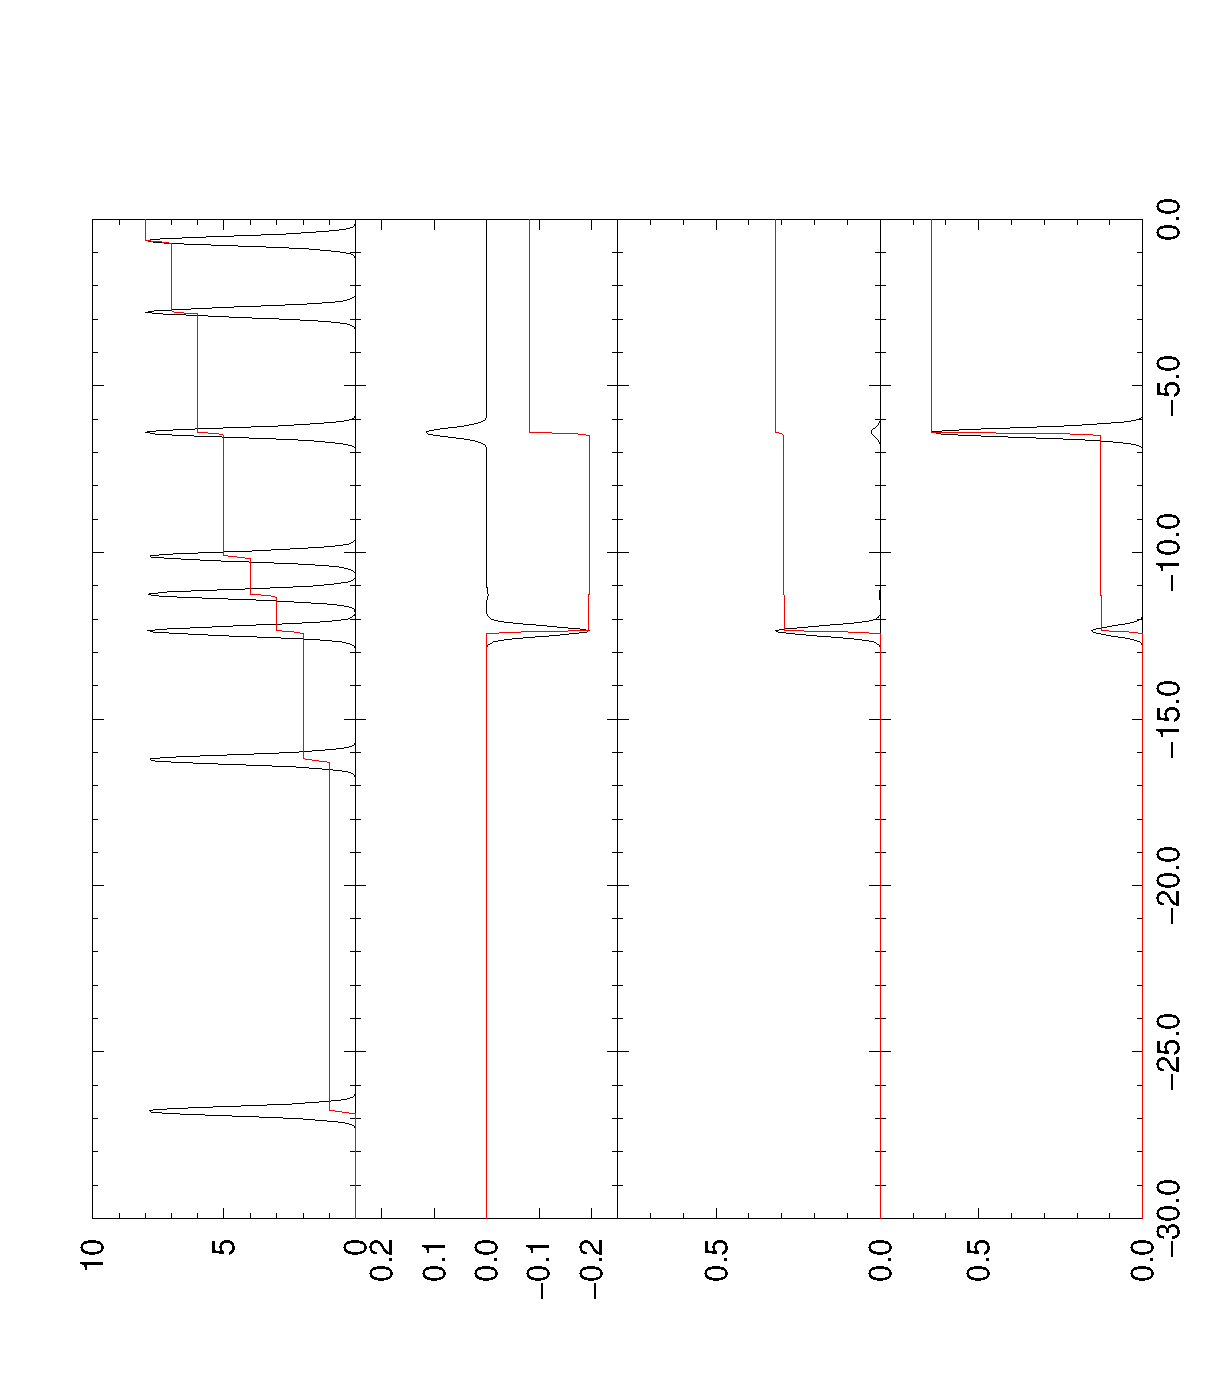
\includegraphics{Figs/h2copdos.eps}}}
}
 \caption{From top to bottom (1) total density of states of the 
   formaldehyde molecule (H$_2$CO). (2) COOP between the p-orbitals
   lying in the plane of the molecule but perpendicular to the CO
   axis. (3) density of states of the p-orbital contributing to the
   COOP on the carbon atom, (4) density of states of the p-orbital
   contributing to the COOP on the oxygen atom}
\label{fig:h2copdos}
\end{figure}

\subsubsection{Orbitals}

The paw\_dos tool works with elementary orbitals, identified by the atom
name, and an abbreviation of an angular momentum such as
\begin{description}
\item[s]An s-orbital with angular dependence 
$Y_s=\sqrt{1\over{4\pi}}$
\item[px]A p-orbital with angular dependence 
$Y_{p_x}=\sqrt{3\over{4\pi}} {x\over{|r|}}$
\item[py]A p-orbital with angular dependence 
$Y_{p_y}=\sqrt{3\over{4\pi}} {y\over{|r|}}$
\item[pz]A p-orbital with angular dependence 
$Y_{p_z}=\sqrt{3\over{4\pi}} {z\over{|r|}}$
\item[dxy]A d-orbital with angular dependence 
$Y_{d_{xy}}=\sqrt{60\over{16\pi}} {{xy}\over{|r|^2}}$
\item[dxz]A d-orbital with angular dependence 
$Y_{d_{xz}}=\sqrt{60\over{16\pi}} {{xz}\over{|r|^2}}$
\item[dyz]A d-orbital with angular dependence 
$Y_{d_{yz}}=\sqrt{60\over{16\pi}} {{yz}\over{|r|^2}}$
\item[d3z2-r2]A d-orbital with angular dependence 
$Y_{d_{3z^2-r^2}}=\sqrt{5\over{16\pi}} {{3z^2-r^2}\over{|r|^2}}$
\item[dx2-y2]A d-orbital with angular dependence 
$Y_{d_{x^2-y^2}}=\sqrt{15\over{16\pi}} {{x^2-y^2}\over{|r|^2}}$
\item[sp] An sp$^1$ orbital pointing in z-direction: 
$\sqrt{1\over{2}}Y_s \phi_s(|r|) + \sqrt{1\over{2}}Y_{p_z}\phi_p(|r|)$
\item[sp2] An sp$^2$ orbital pointing in z-direction: 
$\sqrt{1\over{3}}Y_s\phi_s(|r|) + \sqrt{2\over{3}}Y_{p_z})\phi_p(|r|)$
\item[sp3] An sp$^3$ orbital pointing in z-direction: 
$\sqrt{1\over{4}}Y_s\phi_s(|r|) + \sqrt{3\over{4}}Y_{p_z})\phi_p(|r|)$
\item
\end{description}
where the spherical harmonics are expressed relative to the Cartesian
coordinate system used in the calculation. Instead of projecting on
atomic orbitals as in a Mulliken population analysis, we project here
onto partial waves, that are truncated at the atomic sphere radius.
The atomic sphere radius is approximately 10\% larger than the
covalent radius. (The factor corresponds to the ratio between the
radius of a volume-filling-sphere radius in an fcc crystal and the
corresponding touching-sphere radius.)

More complex orbitals such as bond orbitals can be constructed from
these elementary orbitals by using the block ``!DCNTL!ORBITAL''. The
orbitals are named and can be referred to later by their name.

In practice we define the orbital as
$\sum_i|\chi_i\rangle=\sum_j|\phi_j\rangle c_{j,i}$, and
\begin{eqnarray*}
\langle A\rangle\
&=&\sum_{n,i,j}
\langle\tilde{p}_i|\Psi_n\rangle 
f_n\langle\Psi_n|\tilde{p}_j\rangle\langle\phi_j|A|\phi_l\rangle
\\
&=&\sum_{n,i,j,k,l}
\langle\tilde{p}_k|\Psi_n\rangle 
f_n\langle\Psi_n|\tilde{p}_l\rangle
\frac{c_{l,A}c^*_{i,A}}{\sum_m c^*_{m,A}c_{m,A}}
\langle\phi_i|A|\phi_j\rangle
\frac{c_{j,B}c^*_{k,B}}{\sum_m c^*_{m,B}c_{m,B}}
\end{eqnarray*}
which is divided up into into a density matrix and and a matrix
element according to
\begin{eqnarray*}
D_{B,A}&=&\sum_{n,i,j,k,l}
\frac{c^*_{k,B}}{\sum_m c^*_{m,B}c_{m,B}}
\langle\tilde{p}_k|\Psi_n\rangle 
f_n\langle\Psi_n|\tilde{p}_l\rangle
\frac{c_{l,A}}{\sum_m c^*_{m,A}c_{m,A}}
\\
A_{A,B}&=&\sum_{i,j}c^*_{i,A}\langle\phi_i|A|\phi_j\rangle c_{j,B}
\end{eqnarray*}
Thus if we choose a complete set of orthogonal vectors $\{c_{i,u}\}$,
the total expectation value $A$ is recovered by summing the individual
contributions. For an particular atom and orbital, only the first
partial wave is taken as default.

There is one important remark. The projection done here differs from
the projection 
\begin{eqnarray*}
P&=&\frac{|\chi_u\rangle\langle\chi_u|}{\langle\chi_u|\chi_u\rangle}
\\
&=&|\phi_i\rangle 
\frac{\sum_{i,j} c^*_{i,u}c_{j,u}}
{\sum_{k,l}c^*_{k,u}\langle\phi_k|\phi_l\rangle c_{l,u}}\langle\phi_j|
\end{eqnarray*}
that may be anticipated. In this case we would need a set of vectors
normalized with the overlap between partial waves to obtain the
complete result.


\subsubsection{Matrix elements}

Once the orbitals have been defined, we need to choose the matrix
elements of the PDOS operator. Each matrix element is given a name,
which allows us to use it in further operations. The matrix elements
can be selected in two different ways:

\begin{itemize}

\item To select {\bf diagonal elements} or sums of diagonal elements we use
  the block ``!DCNTL!WEIGHT''. This option allows us to plot the
  total density of states or the angular momentum weights of a
  particular orbital.

\item We can also obtain {\bf off-diagonal elements} using
  ``!DCNTL!COOP'' in order to analyze the bond order or overlap
  populations.

\end{itemize}

%=======================================
\subsubsection{Operations}
%=======================================
Projected charges, spin and eventually spin directions are printed to
the protocol file.  In order to access the data we have to define how
they are to be represented.
\begin{itemize}
\item We can map the density of states on an energy grid and write the
date to a file, so that they can be plotted.
\item The values at a given energy can be printed to the protocol.
\item The values of a given state can be written to a protocol.
\end{itemize}




%==========================================================================
\subsection{Example for the control input file}
%==========================================================================

\begin{verbatim}
!DCNTL
  !FILES 
    !FILE ID='PDOS' EXT=F NAME='~/xx.pdos' !END
    !FILE ID='PROT' EXT=F NAME='stdout'  !END
  !END
  !ORBITAL NAME='SP3(C1-H2)'
    !ORB ATOM='C_1' TYPE='SP3' 
         NNZ='H_2' FAC=1.0 !END
  !END
  !WEIGHT ID='TOTAL' TYPE='TOTAL' !END
  !WEIGHT ID='W(1)'
     !ORB NAME='SP3(C1-H2)' !END
  !END
  !WEIGHT ID='W(2)'
     !ATOM NAME='C_1' TYPE='ALL'!END
  !END
  !COOP   ID='W(3)'
    !ORB1  NAME='SP3(C1-H2)' !END
    !ORB2  ATOM='H_2' TYPE='S' !END
  !END
  !GRID  EMIN[EV]=-18. EMAX[EV]=0. DE[EV]=0.1 
         BROADENING[EV]=0.1 !END
  !OUTPUT ID='W(1)' FILE='~/xx.sp2a' !END
  !OUTPUT ID='W(2)' FILE='~/xx.sp2b' !END
  !OUTPUT ID='W(3)' FILE='~/xx.sp2c' !END
!END
\end{verbatim}

%==========================================================================
\newpage
\subsection{Argument description for the control input file}
%==========================================================================

%----------------------------------------------------------------------
\block{!DCNTL}
%----------------------------------------------------------------------
\brules{optional}
\bdescr{defines the operations done on the system; 
largely independent of the system}

%----------------------------------------------------------------------
\block{!DCNTL!GRID}
%----------------------------------------------------------------------
\brules{optional}
\bdescr{defines the energy grid and energy broadening}

\mbax{\key{EMIN[EV]}
\vdescr{lower bound in eV of the energy interval for density 
of number of states}
\vformat{real} 
\vrules{mandatory}
\vdefault{none}}

\mbax{\key{EMAX[EV]}
\vdescr{upper bound in eV}
\vformat{real} 
\vrules{mandatory}
\vdefault{none}}

\mbax{\key{DE[EV]}
\vdescr{spacing of the grid points}
\vformat{real} 
\vrules{mandatory}
\vdefault{none}}

\mbax{\key{BROADENING[EV]}
\vdescr{density of states are broadened by a Gaussian of the form
$ \exp{-(e/b)^2} $, where $b$ is the broadening.}
\vformat{real} 
\vrules{optional}
\vdefault{none}}

\mbax{\key{SCALEY} 
\vdescr{Allows to scale either the Number of States (NoS) or the
Density of States (DoS) to the same height as the corresponding other
function. Possible values are 'NONE', 'DOS', and 'NOS'. For 'NONE' no 
rescaling takes place. with 'DOS' the DoS is rescaled and for 'NOS', 
the NoS is rescaled.}
\vformat{character} 
\vrules{optional}
\vdefault{'none'}}

%----------------------------------------------------------------------
\block{!DCNTL!FILES}
%----------------------------------------------------------------------
\brules{optional}
\bdescr{Specifies the file names that deviate from the standard values}

%----------------------------------------------------------------------
\block{!DCNTL!FILES!FILE}
%----------------------------------------------------------------------
\brules{optional, multiple}
\bdescr{Specifies one file}

\mbax{\key{ID}
\vdescr{identifier for the file; options are: 
 \begin{description} 
 \item['PROT']protocol file 
   \hfill\break Standard
   extension:'.dprot'
 \item['ERR']error file
   \hfill\break Standard
   extension:'.derr'
 \item['PDOS'] data file produced by the simulation code. Input for
   paw\_dos tool
   \hfill\break Standard extension:'.pdos'
 \item['PDOSOUT']data files ready for plotting.
   \hfill\break Standard extension:'.pdosout'
 \end{description}
}
\vformat{character} 
\vrules{mandatory}
\vdefault{none}}

\mbax{\key{NAME}
\vdescr{filename. Can be the relative file name or an extension to the
  PAW ``root''. Standard output can be specified by NAME='stdout'
  and EXT=.false.}
\vformat{character} 
\vrules{mandatory}
\vdefault{none}}

\mbax{\key{EXT}
\vdescr{.true.: NAME specifies the extension only/ .false.: full name}
\vformat{logical}
\vrules{optional}
\vdefault{.false.}}

%----------------------------------------------------------------------
\block{!DCNTL!ORBITAL}
%----------------------------------------------------------------------
\brules{optional}
\bdescr{defines an orbital}

\mbax{\key{NAME}
\vdescr{names the newly defined orbital !DCNTL!ORBITAL!ORB}
\vformat{character} 
\vrules{mandatory}
\vdefault{none}}

%----------------------------------------------------------------------
\block{!DCNTL!ORBITAL!ORB}
%----------------------------------------------------------------------
\brules{optional, multiple}
\bdescr{select a predefined orbital from which the orbital is built}

\mbax{\key{NAME}
\vdescr{specifies an orbital previously specified by another block
!DCNTL!ORBITAL!ORB}
\vformat{character} 
\vrules{optional; incompatible with atom and type}
\vdefault{none}}

\mbax{\key{ATOM}
\vdescr{atom name on which the orbital resides}
\vformat{character} 
\vrules{optional; incompatible with name}
\vdefault{none}}

\mbax{\key{TYPE} 
\vdescr{orbital type. Can be one of the following.
    'S', 'PX', 'PY', 'PZ', 'DXY', 'D3Z2-R2', 'DXZ', 'DYZ', 'DX2-Y2',
    'SP', 'SP2', 'SP3'. The meaning of these orbitals is described in
    the preceding introduction to the paw\_dos tool.}
\vformat{character} 
\vrules{optional; incompatible with name; mandatory if atom is
  specified.}
\vdefault{none}}

\mbax{\key{IMAG} 
\vdescr{selects the imaginary part of the wave function}
\vformat{logical} 
\vrules{optional}
  specified.}
\vdefault{.false.}}

\mbax{\key{FAC}
\vdescr{Orbital coefficient, with which it contributes the orbital to
be built.}
\vformat{real} 
\vrules{optional}
\vdefault{1.0}}

\mbax{\key{Z}
\vdescr{vector defining the new z-direction to which TYPE refers}
\vformat{real(3)} 
\vrules{optional (overwritten by NNZ)}
\vdefault{0.0,0.0,1.0}}

\mbax{\key{NNZ}
\vdescr{atom name of the atom to which the vector 
defining the new z-direction points}
\vformat{character} 
\vrules{optional; overwrites Z}
\vdefault{see Z}}

\mbax{\key{X}
\vdescr{vector defining the new xz-plane together with z  to which TYPE
refers }
\vformat{real(3)} 
\vrules{optional (overwritten by NNX)}
\vdefault{1.0,0.0,0.0}}

\mbax{\key{NNX}
\vdescr{atom name of the atom to which the vector 
defining the new x-direction points}
\vformat{character} 
\vrules{optional; overwrites X}
\vdefault{see X}}

%----------------------------------------------------------------------
\block{!DCNTL!WEIGHT}
%----------------------------------------------------------------------
\brules{optional,multiple}
\bdescr{defines orbital weights; three ways to specify the weights are
possible
\begin{itemize}
\item specify ``TYPE''; rather unspecific selections such as total
  density of states.
\item specify one or several sub-blocks ``!ATOM''; selects
contributions from different atoms.
\item specify one or several sub-blocks ``!ORB''. Most specific
version, identifying individual orbitals
\end{itemize}
The selection type is not compatible with the other two possibilities.
}

\mbax{\key{ID}
\vdescr{defines the name for this set of matrix elements}
\vformat{character} 
\vrules{mandatory}
\vdefault{none}}

\mbax{\key{TYPE}
\vdescr{specifies how the weights are defined; can be
\begin{description}
\item[``ALL''] sum over all projected density of states
\item[``EMPTY''] weight of the wave function not considered in any projection
\item[``TOTAL''] total density of states
\end{description}}
\vformat{character} 
\vrules{optional; if type is specified, no blocks !atom or !orbs must
be present}
\vdefault{none}}

%----------------------------------------------------------------------
\block{!DCNTL!WEIGHT!ATOM}
%----------------------------------------------------------------------
\brules{optional}
\bdescr{select a predefined orbital from which the orbital is built}

\mbax{\key{NAME}
\vdescr{atom name from which the contribution to this weight is selected}
\vformat{character} 
\vrules{mandatory}
\vdefault{none}}

\mbax{\key{TYPE}
\vdescr{selects the weights from this atom. Can be
\begin{description}
\item[``ALL''] sum over all projected density of states on this atom
\item[``S'']   angular momentum weight for $\ell=0$
\item[``P'']   angular momentum weight for $\ell=1$
\item[``D'']   angular momentum weight for $\ell=2$
\end{description}
}
\vformat{character} 
\vrules{optional}
\vdefault{none}}

\mbax{\key{SPIN}
\vdescr{selects the spin directions in noncollinear calculations. Can be
\begin{description}
\item[``TOTAL''] total density
\item[``X'']   spin density in $x$-direction
\item[``Y'']   spin density in $y$-direction
\item[``Z'']   spin density in $z$-direction
\item[``MAIN'']   spin density in the main spin direction of this atom
\end{description}}
\vformat{character} 
\vrules{optional}
\vdefault{TOTAL}
}

%----------------------------------------------------------------------
\block{!DCNTL!WEIGHT!ORB}
%----------------------------------------------------------------------
\brules{optional}
\bdescr{usage is same as !DCNTL!ORBITAL!ORB}

%----------------------------------------------------------------------
\block{!DCNTL!COOP}
%----------------------------------------------------------------------
\brules{optional} \bdescr{selects a sum of off-diagonal elements of
  the density-of-states operator.  The off-diagonal elements are
  defined by all pairs of orbitals specified in !DCNTL!COOP!ORB1 on
  the one hand and in !DCNTL!COOP!ORB2 on the other hand.}

\mbax{\key{ID}
\vdescr{defines the name for this set of matrix elements}
\vformat{character} 
\vrules{mandatory}
\vdefault{none}}

%----------------------------------------------------------------------
\block{!DCNTL!COOP!ORB1}
%----------------------------------------------------------------------
\brules{optional, multiple} 

\bdescr{selects an orbital for which the off-diagonal elements of the
  density of states operator with the orbitals selected by
  !DCNTL!COOP!ORB2 are to be calculated; usage is same as
  !DCNTL!ORBITAL!ORB}

%----------------------------------------------------------------------
\block{!DCNTL!COOP!ORB2}
%----------------------------------------------------------------------
\brules{optional, multiple} 

\bdescr{selects an orbital for which the off-diagonal elements of the
  density of states operator with the orbitals selected by
  !DCNTL!COOP!ORB1 are to be calculated; usage is same as
  !DCNTL!ORBITAL!ORB}

%----------------------------------------------------------------------
\block{!DCNTL!OUTPUT}
%----------------------------------------------------------------------
\brules{optional,multiple}
\bdescr{selects output of the data; if neither E[EV] nor B are given,
the density of states and the number of states are mapped onto the
energy grid.

The format of the file produced is as follows: Each file have 5
columns with the following content.
\begin{enumerate}
\item energy in eV.
\item density of states (scaled fitting to the sum
of states)
\item integrated density of states (number of states below a given energy).
\item density of states multiplied with actual occupations
\item integrated density of states multiplied with actual occupations
(number of occupied states below a given energy).
\end{enumerate}
In spin-polarized calculations, columns 2-5 refer to spin up. There
are corresponding columns 6-9 for spin down electrons. In
non-collinear calculations there are only 5 columns, which refer to
the total density of states, unless a spin direction has been
explicitely specified.}

\mbax{\key{ID}
\vdescr{defines the name for this set of matrix elements; refers to
ID in block !DCNTL!WEIGHT or !DCNTL!COOP}
\vformat{character} 
\vrules{mandatory}
\vdefault{none}}

\mbax{\key{FILE}
\vdescr{defines the file to which the result shall be written}
\vformat{character} 
\vrules{optional}
\vdefault{the file identified by 'pdosout'}}

\mbax{\key{B}
\vdescr{band index}
\vformat{integer} 
\vrules{optional; incompatible with E[EV]}
\vdefault{none}}

\mbax{\key{E[EV]}
\vdescr{energy}
\vformat{real} 
\vrules{optional; incompatible with B}
\vdefault{none}}

\mbax{\key{S}
\vdescr{spin index}
\vformat{integer} 
\vrules{optional}
\vdefault{all spins}}

\mbax{\key{K}
\vdescr{k-point index}
\vformat{integer} 
\vrules{optional}
\vdefault{all k-points}}


%==========================================================================
\newpage
%\ifthenelse{\boolean{private}}{
\section{The Atomic-Setup program: ``paw\_atom''}
%==========================================================================
The atomic-setup program performs a calculation for an isolated atom
and determines the augmentation-transformation for this atom.

%==========================================================================
\subsection{Command}
%==========================================================================
The calling sequence is

\bigskip\fbox{{\tt paw\_atom} {\it name}}\bigskip

\noindent
where {\it name} is a specifier for the setup. 

%==========================================================================
\subsection{Example for the control input file}
%==========================================================================

\begin{verbatim}
!ACNTL
 !GENERIC ELEMENT='N ' RAUG=2.D0 RBOX=20.D0 !END
 !DFT     TYPE=1 !END
 !GRID    R1=1.056D-4 DEX=0.05 NR=250 !END
 !AECORE
   !STATE L=0 N=1 F=2 !END
 !END
 !VALENCE
   !STATE L=0 N=2 F=2. !END
   !STATE L=1 N=2 F=3. !END
   !STATE L=0 N=3 F=0. !END
 !END
 !VTILDE  TYPE='POLYNOMIAL' RC=1.0 POWER=3 POT(0)=-2.58 !END
 !COMPENSATE RC=0.3 !END
 !PSCORE  TYPE='POLYNOMIAL' RC=1.0 POWER=3 RHO(0)=0.05 !END
 !WAVE L=0 N=2       PSTYPE='HBS' RC=1.0 LAMBDA=6 !END
 !WAVE L=1 N=2       PSTYPE='HBS' RC=1.0 LAMBDA=6 !END
 !WAVE L=0 N=3       PSTYPE='HBS' RC=1.0 LAMBDA=6 !END
!END
!EOB
\end{verbatim}



%==========================================================================
\subsection{Argument description for the control input file ACNTL}
%==========================================================================

%----------------------------------------------------------------------
\block{!ACNTL}
%----------------------------------------------------------------------
\brules{mandatory}
\bdescr{}

%----------------------------------------------------------------------
\block{!ACNTL!GENERIC}
%----------------------------------------------------------------------
\brules{optional}
\bdescr{}

\mbax{\key{ELEMENT}
\vdescr{element symbol.}
\vformat{character} 
\vrules{mandatory}
\vdefault{none}}

\mbax{\key{RAUG}
\vdescr{maximum radius where augmentation operates.}
\vformat{real} 
\vrules{mandatory}
\vdefault{none}}

\mbax{\key{RBOX}
\vdescr{the atom sits in a spherical box with hard walls at r=RBOX.}
\vformat{real} 
\vrules{mandatory}
\vdefault{none}}

%----------------------------------------------------------------------
\block{!ACNTL!DFT}
%----------------------------------------------------------------------
\brules{optional}
\bdescr{}

\mbax{\key{TYPE}
\vdescr{functional type index. see ``!CNTL!DFT''}
\vformat{integer} 
\vrules{mandatory}
\vdefault{none}}

%----------------------------------------------------------------------
\block{!ACNTL!GRID}
%----------------------------------------------------------------------
\brules{optional} \bdescr{Specifies the logarithmic radial grid. It is
  recommended that the default parameters be left as they are, because
  the simulation program can only work with one grid for all setups.}

\mbax{\key{R1}
\vdescr{innermost grid point}
\vformat{real} 
\vrules{optional}
\vdefault{$1.056\times10^{-4}$}}

\mbax{\key{DEX}
\vdescr{logarithmic spacing $\ln(r(i+1)/r(i))$.}
\vformat{real} 
\vrules{optional}
\vdefault{0.05}}

\mbax{\key{NR}
\vdescr{number of grid points}
\vformat{integer} 
\vrules{optional}
\vdefault{250}}

%----------------------------------------------------------------------
\block{!ACNTL!AECORE}
%----------------------------------------------------------------------
\brules{optional}
\bdescr{Defines core states}

%----------------------------------------------------------------------
\block{!ACNTL!AECORE!STATE}
%----------------------------------------------------------------------
\brules{optional}
\bdescr{Defines one state.}

\mbax{\key{L}
\vdescr{main angular momentum quantum number.}
\vformat{integer} 
\vrules{mandatory}
\vdefault{none}}

\mbax{\key{N}
\vdescr{main radial quantum number.}
\vformat{integer} 
\vrules{mandatory}
\vdefault{none}}

\mbax{\key{F}
\vdescr{Occupation. number of electrons in this state}
\vformat{real} 
\vrules{mandatory}
\vdefault{none}}

%----------------------------------------------------------------------
\block{!ACNTL!VALENCE}
%----------------------------------------------------------------------
\brules{optional}
\bdescr{Defines valence states}

%----------------------------------------------------------------------
\block{!ACNTL!VALENCE!STATE}
%----------------------------------------------------------------------
\brules{optional}
\bdescr{Defines one state.}

\mbax{\key{L}
\vdescr{main angular momentum quantum number.}
\vformat{intger} 
\vrules{mandatory}
\vdefault{none}}

\mbax{\key{N}
\vdescr{main radial quantum number.}
\vformat{integer} 
\vrules{mandatory}
\vdefault{none}}

\mbax{\key{F}
\vdescr{Occupation. number of electrons in this state}
\vformat{real} 
\vrules{mandatory}
\vdefault{none}}

%----------------------------------------------------------------------
\block{!ACNTL!VTILDE}
%----------------------------------------------------------------------
\brules{optional}
\bdescr{Defines pseudo-protential. (Do not confuse with the
  pseudopotential of the pseudopotential method.)}

\mbax{\key{TYPE}
\vdescr{pseudization type. Can be ``Polynomial'' or 'HBS'.
\begin{itemize}
\item Polynomial uses a polynomial
$\tilde{v}_{at}(r<r_c)=Ar^n+Br^{n+1}$ and
$\tilde{v}_{at}(r>r_c)=v_{at}(r)$ so that it is differentiable 
and the value at the origin has the value specified by POT(0).
\item HBS uses a cutoff function $k(r)=e^{-(\frac{r}{r_c})^\lambda}$
to obtain the pseudopotential as
$\tilde{v}_{at}(r)=\tilde{v}_0k(r)+[1-k(r)]v_{at}(r)$.
\end{itemize}
}
\vformat{character} 
\vrules{mandatory}
\vdefault{none}}

\mbax{\key{RC}
\vdescr{for POLYNOMIAL: matching radius. For HBS: parameter $r_c$.}
\vformat{real} 
\vrules{mandatory}
\vdefault{none}}

\mbax{\key{POWER} 
\vdescr{for POLYNOMIAL: Order of the polynom used for
  pseudization. For HBS: Parameter $\lambda$. }
\vformat{integer} 
\vrules{mandatory}
\vdefault{none}}

\mbax{\key{POT(0)}
  \vdescr{Value of the pseudo potential at the origin}
\vformat{real} 
\vrules{mandatory}
\vdefault{none}}

%----------------------------------------------------------------------
\block{!ACNTL!COMPENSATE}
%----------------------------------------------------------------------
\brules{optional}
\bdescr{Defines compensation density.}

\mbax{\key{RC}
\vdescr{Gaussian decay parameter $g=\exp(-(\frac{r}{r_c})^2)$.}
\vformat{real} 
\vrules{optional}
\vdefault{0.3}}

%----------------------------------------------------------------------
\block{!ACNTL!PSCORE}
%----------------------------------------------------------------------
\brules{optional}
\bdescr{Defines pseudo core.}

\mbax{\key{TYPE}
\vdescr{pseudization type. Can be ``Polynomial''.}
\vformat{character} 
\vrules{mandatory}
\vdefault{none}}

\mbax{\key{RC}
\vdescr{matching radius.}
\vformat{real} 
\vrules{mandatory}
\vdefault{none}}

\mbax{\key{POWER}
  \vdescr{Order of the polynom used for pseudization}
\vformat{integer} 
\vrules{mandatory}
\vdefault{none}}

\mbax{\key{POT(0)}
  \vdescr{Value of the pseudo potential at the origin}
\vformat{real} 
\vrules{mandatory}
\vdefault{none}}

%----------------------------------------------------------------------
\block{!ACNTL!WAVE}
%----------------------------------------------------------------------
\brules{optional} \bdescr{Defines pseudo wave function. The order of
the states is relevant. (Increasing $n$ and within each n increasing
$\ell$)}

\mbax{\key{L}
\vdescr{main angular momentum quantum number.}
\vformat{integer} 
\vrules{mandatory}
\vdefault{none}}

\mbax{\key{N} 
\vdescr{main radial quantum number. Use only for bound states.}
\vformat{integer} 
\vrules{mandatory if E is not specified. Must not be
specified if E is specified. } 
\vdefault{none}}

\mbax{\key{E}
\vdescr{Energy at which the partial waves are obtained.}
\vformat{integer} 
\vrules{mandatory if N is not specified. Must not be specified if N
  is specified. }
\vdefault{none}}

\mbax{\key{PSTYPE}
\vdescr{pseudization type. Can be ``HBS''. The potential is varied by
  a potential $\exp(-(r/r_c)^\lambda$ with a variable scaling factor.}
\vformat{character} 
\vrules{mandatory}
\vdefault{none}}

\mbax{\key{RC}
\vdescr{matching radius.}
\vformat{real} 
\vrules{mandatory}
\vdefault{none}}

\mbax{\key{LAMBDA}
  \vdescr{}
\vformat{integer} 
\vrules{mandatory}
\vdefault{none}}

%}{} % end of \ifthenelse

%==========================================================================
\newpage
\section{The Structure Pre-Optimization Tool: paw\_preopt}
%==========================================================================

The paw\_preopt tool allows to perform a fast but inaccurate structure
pre-optimization based on force-field molecular dynamics. It reads the
structure input file (\verb'case.strc') and tries to find bonds in the
given structure using the covalent radii of the atoms. Then it tries
to find suitable parameterizations for the atoms using the universal
force field (UFF) \cite{UFF}. (See also section \ref{sec:UFF}.) Bonds
and force field parameterizations can also be provided via the input
files. Atoms to be frozen can be specified.

Using the parameterization it optimizes the geometry (currently) using
the conjugate gradient line search algorithm which is also used in
QM-MM coupling in the main simulation program. Atom positions after
optimization are printed to the protocol file and may be used as
starting point for a PAW simulation.

Atoms can be frozen during the optimization. No other constraints can
be applied. Freezing can either be done via the keywords
!PCNTL!FREEZEONLY and !PCNTL!MOVEONLY or via the keyword FREEZE=T in
the !ATOM block of the structure input file. The latter will be
ignored by the main PAW simulation program.

%==========================================================================
\subsection{Command}
%==========================================================================

The calling sequence is

\bigskip\fbox{{\tt paw\_preopt.x} {\it controlfile}}\bigskip

\noindent
where {\it controlfile} is the file name of the control input file for
the paw\_preopt tool. I recommend the extension ``.pcntl''.

%==========================================================================
\subsection{Example for the control input file}
%==========================================================================

\begin{verbatim}
!PCNTL
  !FILES
    !FILE ID='xyz' NAME='optimized.xyz' !END
  !END
  !GENERIC
    TRACE=F
    TOL=0.0001
    NSTEPS=10000
  !END
  !OUTPUT
     PRINTATOMS=T
     PRINTBONDS=T
     WARNFF=T
     XYZOUT=T
  !END
  !FREEZEONLY 
    COMMENT='Not used if MOVEONLY is present.'
    !ATOM NAME='MO1' !END
    !ATOM PART='FE' !END
  !END
  !MOVEONLY
     !ATOM_OFF PART='H_nh' !END
     !ATOM NAME='N_nh41' !END
     !ATOM NAME='H_nh43' !END
     !ATOM NAME='H_nh44' !END
     !ATOM NAME='H_nh45' !END
  !END
!END
!EOB
\end{verbatim}

Please note that a keyword COMMENT is ignored by all PAW
programs. Thus it can be used to add comments to the input files.

%==========================================================================
%\newpage
\subsection{Argument description for the control input file}
%==========================================================================

%----------------------------------------------------------------------
\block{!PCNTL}
%----------------------------------------------------------------------
\brules{mandatory}
\bdescr{defines the operations done on the system; 
largely independent of the system}

%----------------------------------------------------------------------
\block{!PCNTL!GENERIC}
%----------------------------------------------------------------------
\brules{optional}
\bdescr{defines optimization parameters (and use of the trace)}

\mbax{\key{TRACE}
\vdescr{writes information on the calls of subroutines to standard output}
\vformat{logical} 
\vrules{optional}
\vdefault{F}}

\mbax{\key{TOL}
\vdescr{tolerance of the maximal component of the force on atoms in 
  the convergence cycles}
\vformat{real} 
\vrules{optional}
\vdefault{10$^{-4}$}}

\mbax{\key{NSTEPS}
\vdescr{maximal number of steps for the convergence. After that number
  the structure optimization is stopped no matter if the forces have
  become smaller than TOL. A statement on the convergence will be
  written to the protocol.}
\vformat{integer} 
\vrules{optional}
\vdefault{1000}}

%----------------------------------------------------------------------
\block{!PCNTL!FILES}
%----------------------------------------------------------------------
\brules{optional}
\bdescr{specifies the file names that deviate from the standard values}

%----------------------------------------------------------------------
\block{!PCNTL!FILES!FILE}
%----------------------------------------------------------------------
\brules{optional, multiple}
\bdescr{Specifies one file}

\mbax{\key{ID}
\vdescr{identifier for the file; options are: 
 \begin{description} 
 \item['PROT']protocol file \hfill\break Standard extension:'.pprot'
 \item['STRC'] The structure file as used by the simulation code. Used
   for the input structure. \hfill\break Standard extension:'.strc'
 \item['XYZ'] data file with the resulting optimized structure
   \hfill\break Standard extension:'.xyz'
 \end{description}
}
\vformat{character} 
\vrules{mandatory}
\vdefault{none}}

\mbax{\key{NAME}
\vdescr{filename. Can be the relative file name or an extension to the
  PAW ``root''. Standard output can be specified by NAME='stdout'
  and EXT=.false.}
\vformat{character} 
\vrules{mandatory}
\vdefault{none}}

\mbax{\key{EXT}
\vdescr{T: NAME specifies the extension only. F: full name}
\vformat{logical}
\vrules{optional}
\vdefault{F (false)}}

%----------------------------------------------------------------------
\block{!PCNTL!OUTPUT}
%----------------------------------------------------------------------
\brules{optional}
\bdescr{specifies which information should be written to the protocol}

\mbax{\key{PRINTATOMS}
\vdescr{information on the used atom parameterization and freezing is
  written to the protocol}
\vformat{logical} 
\vrules{optional}
\vdefault{T}}

\mbax{\key{PRINTBONDS}
\vdescr{information on the used bonds is
  written to the protocol}
\vformat{logical} 
\vrules{optional}
\vdefault{T}}

\mbax{\key{WARNFF}
\vdescr{paw\_preopt tries to find best-suiting force fields for the
  atoms. However, in some cases it cannot decide which parameterization
  will be the best. If T in these cases a warning will be printed to
  the protocol.}
\vformat{logical} 
\vrules{optional}
\vdefault{T}}

\mbax{\key{XYZOUT}
\vdescr{should an xyz-file of the resulting structure be created?}
\vformat{logical} 
\vrules{optional}
\vdefault{T}}


%----------------------------------------------------------------------
\block{!PCNTL!FREEZEONLY}
%----------------------------------------------------------------------
\brules{optional, not used if !PCNTL!MOVEONLY is present}
\bdescr{sets freezing of all atoms but those specified in this block
  to false. May be overwritten for single atoms by !STRC!ATOM:FREEZE}

\mbax{\key{NAME}
\vdescr{specifies an atom name}
\vformat{character} 
\vrules{optional, multiple}
\vdefault{none}}

\mbax{\key{PART}
\vdescr{Specifies a part of an atom name. All atoms containing this
  string are used. Case is ignored.}
\vformat{character} 
\vrules{optional, multiple}
\vdefault{none}}

%----------------------------------------------------------------------
\block{!PCNTL!MOVEONLY}
%----------------------------------------------------------------------
\brules{optional, overwrites !PCNTL!FREEZEONLY}
\bdescr{sets freezing of all atoms but those specified in this block
  to true. May be overwritten for single atoms by !STRC!ATOM:FREEZE}

\mbax{\key{NAME}
\vdescr{specifies an atom name}
\vformat{character} 
\vrules{optional, multiple}
\vdefault{none}}

\mbax{\key{PART}
\vdescr{Specifies a part of an atom name. All atoms containing this
  string are used. Case is ignored.}
\vformat{character} 
\vrules{optional, multiple}
\vdefault{none}}

%==========================================================================
%\newpage
\subsection{Argument description for the structure input file}
%==========================================================================

The atomic structure is read from a structure input file which has the
same syntax as for the main simulation code. However, a few keywords
are used which are ignored by the main simulation code. The keyword
!STRC!GENERIC:LUNIT is mandatory.

%----------------------------------------------------------------------
\block{!STRC!ATOM}
%----------------------------------------------------------------------
\brules{mandatory,multiple}
\bdescr{usage is same as in the main simulation code. Keywords R, SP
  and NAME are used. Additional keywords are:}

\mbax{\key{FFTYPE}
\vdescr{Force field type used for this atom. This keyword can be used
  to overwrite the suggestion of the program. Possible force fields
  can be found in section~\ref{sec:UFF} on page~\pageref{sec:uff}.}
\vformat{character} 
\vrules{optional}
\vdefault{depending on the atom type and the number of bonds to that atom}}

\mbax{\key{FREEZE}
\vdescr{freeze this atom}
\vformat{logical} 
\vrules{optional}
\vdefault{F}}

%----------------------------------------------------------------------
\block{!STRC!BOND}
%----------------------------------------------------------------------
\brules{optional,multiple}
\bdescr{Overwrite the suggestion of the program for bonds between the
  atoms. Not yet implemented.}

 
%==========================================================================
\newpage
\section{Specifications of formatted and unformatted output data files}
%==========================================================================
%==========================================================================
\subsection{Protocoll}
%==========================================================================
One-particle energies: The eigenvalues of the Hamiltonian in the basis
of the wave function are printed, unless dynamical occupations are
selected (i.e. \texttt{!CONTROL!MERMIN}). In this latter case, the
diagonal elements of the Hamiltonian are printed. The one-particle
energies are printed in eV. The occupations are printed without the
geometric weight, but include spin degeneracy, so that for a non-spin
polarized calculation the maximum allowed occupation is two.



%==========================================================================
\subsection{waveplot}
%==========================================================================
The file waveplot is used to provide a wave function or a density on
a real space grid. From there it has to be converted into a format
ready for visualization, which can be done using the ``waveplot'' tool.
A waveplot file is created by selecting ``!CNTL!ANALYSE!WAVE'' in the
control input file.


The file is written as follows:
\small{
\begin{verbatim}
CHARACTER(*) :: TITLE     ! user defined comment
INTEGER(4)   :: NAT       ! number of atoms
REAL(8)      :: RBAS(3,3) ! lattice vectors (xyzxyzxyz)
REAL(8)      :: POS(3,NAT)! atomic positions
REAL(8)      :: Z(NAT)    ! atomic numbers 
REAL(8)      :: Q(NAT)    ! point charges
CHARACTER(32):: NAME(NAT) ! atom name (see file strc_out)
                          ! number of grid points along 
INTEGER(4)   :: NR1       !        first direction
INTEGER(4)   :: NR2       !        second
INTEGER(4)   :: NR3       !        third
REAL(8)      :: WAVE(NR1,NR2,NR3) ! density or wave function 
                                  ! on the real space grid
WRITE(UNIT)'WAVEPLOT',LEN(TITLE)
WRITE(UNIT)TITLE
WRITE(UNIT)RBAS,NAT
WRITE(UNIT)NR1,NR2,NR3
WRITE(UNIT)NAME
WRITE(UNIT)Z
WRITE(UNIT)POS
WRITE(UNIT)Q
WRITE(UNIT)WAVE
WRITE(UNIT)'END OF FILE'
\end{verbatim}
}

The coordinates of the density or wave with $(i_1,i_2,i_3)$ are 
\begin{equation}
  x_i=\sum_{i=1}^{3} {\rm RBAS}_{i,j}{{i_i-1}\over{{\rm NR}i}} 
\end{equation}

%==========================================================================
\subsection{Projected density of states files}
%==========================================================================
\begin{verbatim}
INTEGER(4)  :: NAT   !#(ATOMS)
INTEGER(4)  :: NSP   !#(ATOM TYPES)
INTEGER(4)  :: NKPT  !#(K-POINTS)
INTEGER(4)  :: NSPIN !#(SPINS)
INTEGER(4)  :: NDIM  !#(SPINOR COMPONENTS)
INTEGER(4)  :: NPRO  !#(PROJECTIONS PER STATE)
INTEGER(4)  :: LNXX  !MAX#(PARTIAL WAVES PER ATOM (L,N))
INTEGER(4)  :: LNX(NSP)      !#(PARTIAL WAVES PER ATOM (L,N))
INTEGER(4)  :: LOX(LNXX,NSP) !MAIN QUANTUM NUMBER
INTEGER(4)  :: ISPECIES(NAT) !ATOM TYPE
REAL(8)     :: RBAS(3,3)     !LATTICE VECTORS
REAL(8)     :: R0(3,NAT)     !ATOMIC POSITIONS 
INTEGER(4)  :: IZ            !ATOMIC NUMBER
REAL(8)     :: RAD           !``ASA RADIUS''
REAL(8)     :: VAL(LNXX)     ! AEPHI(RAD)
REAL(8)     :: DER(LNXX)     ! DAEPHI/DR(RAD)
REAL(8)     :: OV(LNXX,LNXX) ! <AEPHI|AEPHI> WITHIN RAD
REAL(8)     :: XK(3,NKPT)    ! K-POINT IN RELATIVE COORDINATES
INTEGER(4)  :: NB            ! #(BANDS)
REAL(8)     :: EIG(NB,NSPIN,NKPT)               ! EIGENVALUES
COMPLEX(8)  :: PROJ(NDIM,NPRO,NB,NSPIN,NKPT)    ! PROJECTIONS
!**************************************************************
WRITE(NFIL)NAT,NSP,NKPT,NSPIN,NDIM,NPRO,LNXX
WRITE(NFIL)LNX(:),LOX(:,:),ISPECIES(:)
WRITE(NFIL)RBAS(:,:),R0(:,:)
DO ISP=1,NSP
   WRITE(NFIL)IZ,RAD,VAL(1:LNX(ISP)),DER(1:LNX(ISP)) &
&                                   ,OV(1:LNX(ISP),1:LNX(ISP))
ENDDO
DO IKPT=1,NKPT
  DO ISPIN=1,NSPIN
    WRITE(NFIL)XK(:,IKPT),NB
    DO IB=1,NB
      WRITE(NFIL)EIG,PROJ(:,:)
    ENDDO
  ENDDO
ENDDO
\end{verbatim}


%==========================================================================
\subsection{Trajectory files}
%==========================================================================
Trajectory files are used to monitor variables step by step. 

The file is written as follows:
\begin{verbatim}
INTEGER(4)  :: ISTEP1    !
INTEGER(4)  :: ISTEP2
INTEGER(4)  :: LEN
REAL(8)     :: TIME(ISTEP1:ISTEP2)
REAL(8)     :: ARRAY(LEN,ISTEP1:ISTEP2)
!
DO ISTEP=ISTEP1,ISTEP2
  WRITE(UNIT)ISTEP,TIME(ISTEP),LEN,ARRAY(:,ISTEP)
ENDDO
\end{verbatim}

Here ``istep'' is the number of the time step, consistent with the
protocol file. 

%==========================================================================
\subsubsection{Position Trajectory}
%==========================================================================
In the position trajectory ``{\it root}\_r.tra'', LEN is four times
the number of atoms and array are the atomic positions starting x,y,z
of the first atom, x,y,z of the second and so fourth until the last
atom followed by the point charges on the atoms beginning with the
first atom.

%==========================================================================
\newpage
\section{Units and constants}
\label{constants}
%==========================================================================

The program works in Cartesian coordinates using Hartree atomic units
\begin{equation}
\hbar=e=m_e=4\pi\epsilon_0=1 \ .
\end{equation}
Angles are given in radian ($2\pi~{\rm radian}=360~\deg$).

The following list is produced by the CONSTANTS object.  The data are
based on a values recommended by The Commitee on Data for Science and
Technology (CODATA) \cite{Constants}.
\begin{verbatim}
UNITS AND CONSTANTS IN ATOMIC HARTREE UNITS:
--------------------------------------------
     NAME           VALUE        :DESCRIPTION
PI.............=    3.141593     :PI
HBAR...........=    1.000000     :A.U. FOR ANGULAR MOMENTUM
E..............=    1.000000     :ELEMENTARY CHARGE
ME.............=    1.000000     :ELECTRON MASS
EPSILON0.......=    7.957747E-02 :PERMITIVITY OF VACUUM
ALPHA..........=    7.297353E-03 :FINE STRUCTURE CONSTANT
ABOHR..........=    1.000000     :BOHR RADIUS
TAU0...........=    1.000000     :A.U. FOR TIME
HARTREE........=    1.000000     :HARTREE ENERGY UNIT
C..............=  137.035989     :SPEED OF LIGHT
MU0............=    6.691764E-04 :PERMEABILITY OF VACCUM
BOHRMAGNETON...=    0.500000     :BOHR MAGNETON
NUCLEARMAGNETON=    2.723085E-04 :NUCLEAR MAGNETON
GE.............=    2.002319     :ELECRON GYROMAGNETIC RATIO
KG.............=    1.097768E+30 :KILOGRAMM      
SECOND.........=    4.134137E+16 :SECOND     
METER..........=    1.889726E+10 :METER
AMPERE.........=  150.974819     :AMPERE           
MOL............=    6.022137E+23 :MOLE
KB.............=    3.166679E-06 :BOLTZMANN CONSTANT IN A.U.
NEWTON.........=    1.213779E+07 :NEWTON
JOULE..........=    2.293710E+17 :JOULE
COULOMB........=    6.241506E+18 :COULOMB
VOLT...........=    3.674931E-02 :VOLT
TESLA..........=    4.254381E-06 :TESLA
GAUSS..........=    4.254381E-10 :GAUSS
RY.............=    0.500000     :RYDBERG ENERGY UNIT
EV.............=    3.674931E-02 :ELECTRON VOLT
ANGSTROM.......=    1.889726     :ANGSTROM
KJ/MOL.........=    3.808798E-04 :KILOJOULE PER MOLE
KCAL/MOL.......=    1.593601E-03 :KILOCALORIE PER MOLE
U..............=    1.822889E+03 :atomic MASS UNIT 
DEBYE..........=    0.393430     :DEBYE


CONVERSION FACTORS AN CONSTANTS:
--------------------------------
--------- ATOMIC UNITS ---------------------------------
QE.....................=    1.000000     :A.U.
HBAR...................=    1.000000     :A.U.
ME.....................=    1.000000     :A.U.
HARTREE................=    1.000000     :A.U.
ABOHR..................=    1.000000     :A.U.
1/ALPHA................=  137.035989     :
EPSILON0...............=    7.957747E-02 :
MU0....................=    6.691764E-04 :
C......................=  137.035989     :ABOHR/TAU0
KB.....................=    3.166679E-06 :HARTREE
--------- CONVERSION FROM SI TO ATOMIC UNITS -----------
MOL....................=    6.022137E+23 :
METER..................=    1.889726E+10 :ABOHR
SECOND.................=    4.134137E+16 :TAU0
JOULE..................=    2.293710E+17 :HARTREE
KG.....................=    1.097768E+30 :ME
C......................=    2.997925E+08 :METER/SECOND
--------- CONVERSION FROM ATOMIC TO SI UNITS -----------
ABOHR..................=    5.291772E-11 :METER
TAU0...................=    2.418884E-17 :SECOND
ME.....................=    9.109390E-31 :KG
E......................=    1.602177E-19 :COULOMB
HBAR...................=    1.054573E-34 :JOULE*SECOND
--------- LENGTH CONVERSIONS ---------------------------
ANGSTROM...............=    1.889726     :ABOHR
ABOHR..................=    0.529177     :ANGSTROM
ABOHR..................=    5.291772E-11 :METER
METER..................=    1.889726E+10 :ABOHR
--------- TIME CONVERSIONS -----------------------------
TAU0...................=    2.418884E-17 :SECOND
TAU0...................=    2.418884E-02 :FEMTO SECOND
PICO SECOND............=    4.134137E+04 :TAU0
--------- ENERGY CONVERSIONS ---------------------------
273.15 KB..............=    2.353727E-02 :EV
EV.....................=   96.485309     :KJ/MOL
HARTREE................=    2.625500E+03 :KJ/MOL
EV.....................=   23.060542     :KCAL/MOL
HARTREE................=  627.509556     :KCAL/MOL
KJ/MOL.................=    1.036427E-02 :EV
KCAL/MOL...............=    4.336411E-02 :EV
HARTREE................=   27.211396     :EV
RY.....................=    0.500000     :HARTREE
--------- MASS CONVERSIONS -----------------------------
U......................=    1.660540E-27 :KG
U......................=    1.822889E+03 :ME
--------- CHARGE CONVERSIONS ---------------------------
QE.....................=    1.602177E-19 :COULOMB
COULOMB................=    6.241506E+18 :QE
--------- OTHER CONVERSIONS ----------------------------
DEBYE..................=    0.393430     :E*ABOHR
E*ABOHR................=    2.541748     :DEBYE
E_ZPV/T[PSEC]..........=    7.599149E-05 :HARTREE
E_ZPV/T[PSEC]..........=    2.067835E-03 :EV
E_ZPE/(1/LAMBDA)[CM**-1=    6.199212E-05 :EV
E_ZPE/(1/LAMBBDA)[CM**-=    2.278168E-06 :HARTREE
(1/LAMBDA).............=   33.356410     :CM**-1/T[PSEC]

Scale factors :
---------------
FEMTO..........=    1.000000E-15 :FEMTO=1.D-15
PICO...........=    1.000000E-12 :PICO=1.D-12
NANO...........=    1.000000E-09 :NANO=1.D-9
MICRO..........=    1.000000E-06 :MICRO=1.D-6
MILLI..........=    1.000000E-03 :MILLI=1.D-3
KILO...........=    1.000000E+03 :KILO=1.D+3
MEGA...........=    1.000000E+06 :MEGA=1.D+6
GIGA...........=    1.000000E+09 :GIGA=1.D+9
TERA...........=    1.000000E+12 :TERA=1.D+12
PETA...........=    1.000000E+15 :PETA=1.D+15
\end{verbatim}

%===================================================================
\newpage
\subsection{Vibrations}
%===================================================================

Vibrational freqencies and optical absorption energies are frequenty measured
via the frequency or wave-length of the absorbed light. The frequency or
energy is measured in wave-numbers $\bar{\nu}=1/L$ defined as the inverse
of the wavelength $L$. (The wave number is the number of times an
oscillation of a light wave fitswithin a given length interval.) It is
measured in units of cm$^{-1}$. Here we provide the conversion of wave numbers
into energies, frequencies, etc.


First we convert the wave number into a frequency $\omega=2\pi/T$ where $T$ is
the time of a full oscillation. 

We use the dispersion relation of light $\omega=c|k|$, where $c$ is the speed
of light. $\omega=\frac{2\pi}{T}$ is the frequency and
$|\vec{k}|=\frac{2\pi}{L}$ is the absolute value of the wave vector. $T$ is the
time for one full period at a given position and $L$ is the length for one
full period at a given time.

From the dispersion relation we calculate the 
the frequency $\omega=2\pi/T$ and the 
\begin{eqnarray}
|k|&=&\frac{2\pi}{\bar{\nu}}
\label{eq:kofbarnu}
\\
L&=&\frac{1}{\bar{\nu}}
\label{eq:wavelengthofbarnu}
\\
\omega&=&c|k|=c2\pi/L=2\pi c\bar{\nu}
\label{eq:omegaofbarnu}
\\
T&=&\frac{2\pi}{\omega}=\frac{1}{c\bar{\nu}}
\label{eq:periodofbarnu}
\end{eqnarray}
The connection to the energy is given by $E=\hbar\omega$, where $E$ is the
energy of the absorbed or emmited photon with frequency $\omega$. It is the
energy difference between the energy levels of the corresponding transition.
\begin{eqnarray}
E&=&\hbar\omega=2\pi\hbar c\bar{\nu}
\label{eq:eofomega}
\end{eqnarray}
Finally we would like to know the force constant $C$ for a harmonic oscillator
producing these level spacings. 
\begin{eqnarray}
M\ddot{x}&=&-CX
\qquad\Rightarrow\qquad \omega= \sqrt{\frac{C}{M}}
\nonumber\\
C&=&M\omega^2=M4\pi^2c^2\bar{\nu}^2
\end{eqnarray}

Let us now evaluate the conversion factors
\begin{eqnarray*}
T[ps]&\stackrel{\textrm{Eq.~\ref{eq:periodofbarnu}}}{=}& \frac{1}{c[a_0/\tau_0]\bar{\nu}[cm^{-1}] } 
\frac{\tau_0}{ps}\cdot\frac{cm}{a_0}
\\
&=&
\left(\frac{1}{137.035989}\right)\cdot
\left(\frac{1}{10^{-12}\cdot 4.134137\times 10^{16}}\right)
\cdot\left(10^{-2}\cdot 1.889726\times 10^{10}\right)
\frac{1}{\bar{\nu}[cm^{-1}] } 
\\
&=&
\frac{1.889726}{1.37035989\cdot4.134137}\cdot10^{-2+12-16-2+10}
\frac{1}{\bar{\nu}[cm^{-1}] } 
\\
&=&0.3335640485\times10^{2}
\frac{1}{\bar{\nu}[cm^{-1}] } 
=33.35640485\frac{1}{\bar{\nu}[cm^{-1}] }
\\
T[a.u.]&=&1.379\times 10^6 \frac{1}{\bar{\nu}[cm^{-1}] }
\end{eqnarray*}
Note that we can read $T[ps]$ as $T/ps$ if we $ps$ is the value of a
pico-second in the unit system of choice.

The energy is obtained from Eq.~\ref{eq:eofomega} as
\begin{eqnarray*}
E[a.u.]&=&\hbar\omega=2\pi\hbar[a.u.] c[a.u.]\frac{a_0}{m}
10^2
\bar{\nu}[cm^{-1}]
\\
&=&2\pi\times 137.035989\frac{1}{1.889726\times 10^{10}}10^2\bar{\nu}[cm^{-1}]
\\
&=&2\pi\times 137.035989\frac{1}{1.889726\times 10^{10}}10^2\bar{\nu}[cm^{-1}]
\\
&=&4.556335\times10^{-6}\bar{\nu}[cm^{-1}]
\\
E[eV]&=&1.23984242\times10^{-4}\bar{\nu}[cm^{-1}]
\end{eqnarray*}
As crosscheck we may use that the ground state of the hydrogen atom lies at
$-\frac{1}{2}$~H=-13.6~eV corresponds to $\bar{\nu}$=-109678~cm$^{-1}$. This
number is the Rydberg constant. (see Demtr\"oder, Experimentalphysik 3;
Springer Verlag p.102)

Here i summarize the main vibrational modes
\begin{center}
\begin{tabular}{|c|c|}
\hline
Vibr. Mode & $\bar{\nu}[cm^{-1}]$\\ 
\hline
H-H Stretch & $\approx$ 4000\\
C-H Stretch & 2800-3999 \\
C-H Bend    & 1400-1500 \\
C-C Stretch & 1500-1750 \\
\hline
\end{tabular}
\end{center}
The hydrogen stretch vibration has a period of about 350~$\tau_0$ or 8.3~fs.
The optical phonon in bulk silicon has a frequency of about 14~THz, which
corresponds to $\bar{\nu}=450-500$~cm$^{-1}$.

%===================================================================
\subsection{Magnetic hyperfine parameters}
%===================================================================

The hyperfine parameters measure the splitting of several transitions,
each of which switches the spin of an electron, and preserves the spin
of the nucleus. The energy of a nucleus in the magnetic field of the
electronic spin density is
\begin{displaymath}
E=m^N B^N
\end{displaymath}
where $m^N$ is the magnetic moment of the nucleus, and $B^N$ is the
hyperfine field created by the electronic spin density. (The hyperfine
field is a kind of effective magnetic field). When the electron spin
is flipped by an electronic transition, the transition energy is
$\hbar\omega=\hbar\omega_0+2m^NB^N$. For different spin quantum
numbers $S^N_z$, we obtain transitions
\begin{equation}
\hbar\omega(S^N_z)=\hbar\omega_0+2\frac{m^N}{S^N}B^N S^N_z
\end{equation}
from which follows the splitting of neighboring levels
\begin{equation}
\Delta E=\Delta \hbar\omega(S^N_z)=2\hbar\frac{m^N}{S^N}B^N 
\end{equation}
with $S^N$ being the nuclear spin with values $0,1/2\hbar,\hbar,..$,
depending on the nucleus.

The quantity $\gamma_N=m^N/S^N$ is called the gyromagnetic ratio of
the nucleus.  The nuclear magnetic moment is typically given units of
nuclear magnetons $\mu_N=(m_e/m_p)\mu_B$, where $m_e$ is the electron
mass, $m_p$ is the proton mass, and $\mu_B=\frac{e\hbar}{2m_e}$ is the
Bohr magneton.

In the literature the hyperfine splitting is often converted into a
frequency $\nu$ using the relation $\Delta E=h\nu$. The frequency is
expressed typically in MHz. Another term used for MHz is Mc$/$s, i.e.
megacycles per second.
\begin{eqnarray*}
\nu&=&\frac{\Delta E}{2\pi\hbar} 
=\frac{m^N B^N}{\pi S^N}
\\
&=&
\frac{m^N[\mu_N]B^N[{\rm T}]}{S^N[\hbar]}
\times\frac{\mu_N {\rm T}}{\pi \hbar {\rm MHz}}\ {\rm MHz}
\\
&=&\frac{m^N[\mu_N]B^N[{\rm T}]}{S^N[\hbar]} 15.24518048\ {\rm MHz}
\end{eqnarray*}
The frequency is often converted in wavenumbers using the relation
$\frac{1}{l}=\frac{\nu}{c}$.
\begin{eqnarray*}
\frac{1}{l}&=&
\frac{m^N[\mu_N]B^N[{\rm T}]}{S^N[\hbar]} \times\frac{\mu_N {\rm T}
  10^{-2}{\rm m}}{\pi c\hbar
  }\ {\rm cm}^{-1}
\\
&=&
\frac{m^N[\mu_N]B^N[T]}{S^N[\hbar]} \times 5.085135181\times 10^{-4}\ {\rm cm}^{-1}
\end{eqnarray*}


The energy of the magnetic hyperfine splitting is often converted into
a effective magnetic field $B^e$ acting on the electrons via
\begin{displaymath}
\Delta E=g_e\mu_B B^e
\end{displaymath}
where $\mu_B$ is the Bohr magneton, $g_e$ is the g-factor of the free
electron. While the g-factor of the electron is slightly larger than
2, its value is set exactly to 2. The term $g_e\mu_B$ is twice the
magnetic moment of the electron. 
\begin{eqnarray*}
B^e&=&\frac{\Delta E}{g_e\mu_B}=\frac{2\hbar m_N B_N}{s_N g_e\mu_B}
\\
&=&\frac{m_N[\mu_N]B_N[{\rm T}]}{s_N[\hbar]}\times 
\frac{2\hbar\mu_N T}{\hbar 2\mu_B {\rm T}}\ {\rm T} 
\\
&=& \frac{m_N[\mu_N]B_N[{\rm T}]}{s_N[\hbar]}\times 0.544617\ {\rm mT}
\end{eqnarray*}
The magnetic field is either given in
milliTesla, in Oersted or in Gauss (1~Oe=1~gauss=10$^{-4}$~T).

%==========================================================================
\newpage
\section{Periodic Table}
%==========================================================================
Atomic masses according to IUPAC 1985 (Pure Appl. Chem. 1985, 58,
1677-1692). Length units are in atomic units. ``R(COV)'' is the covalent radius.
``R(ASA)'' is the covalent radius scaled up by about 10\%, consistent
with the scaling between touching and volume filling spheres in an fcc
solid. ``R(VDW)'' is the Van der Waals radius \cite{UFF}.

\small
\begin{verbatim}
SY   Z  MASS[U] R(COV) R(ASA) R(VDW) CONFIGURATION  #(NODES)
------------------------------------------------------------
H    1    1.008  0.605  0.668  5.454 [0 ]S1                   
HE   2    4.003  1.757  1.943  4.464 [0 ]S2                   
LI   3    6.941  2.324  2.569  4.632 [HE]S1         S1        
BE   4    9.012  1.701  1.880  5.187 [HE]S2         S1        
B    5   10.811  1.550  1.713  7.716 [HE]S2P1       S1        
C    6   12.110  1.455  1.608  7.277 [HE]S2P2       S1        
N    7   14.007  1.417  1.567  6.916 [HE]S2P3       S1        
O    8   15.999  1.380  1.525  6.614 [HE]S2P4       S1        
F    9   18.998  1.361  1.504  6.357 [HE]S2P5       S1        
NE  10   20.180  1.342  1.483  6.128 [HE]S2P6       S1        
NA  11   22.990  2.910  3.217  5.637 [NE]S1         S2P1      
MG  12   24.305  2.570  2.841  5.709 [NE]S2         S2P1      
AL  13   26.982  2.230  2.465  8.502 [NE]S2P1       S2P1      
SI  14   28.086  2.098  2.319  8.116 [NE]S2P2       S2P1      
P   15   30.974  2.003  2.214  7.837 [NE]S2P3       S2P1      
S   16   32.066  1.928  2.131  7.625 [NE]S2P4       S2P1      
CL  17   35.453  1.871  2.068  7.459 [NE]S2P5       S2P1      
AR  18   39.948  1.852  2.047  7.309 [NE]S2P6       S2P1      
K   19   39.098  3.836  4.240  7.204 [AR]S1         S3P2      
CA  20   40.078  3.288  3.634  6.423 [AR]S2         S3P2      
SC  21   44.956  2.721  3.008  6.227 [AR]S2D1       S3P2      
TI  22   47.880  2.494  2.757  6.000 [AR]S2D2       S3P2      
V   23   50.942  2.305  2.548  5.941 [AR]S2D3       S3P2      
CR  24   51.996  2.230  2.465  5.713 [AR]S1D5       S3P2      
MN  25   54.938  2.211  2.444  5.595 [AR]S2D5       S3P2      
FE  26   55.847  2.211  2.444  5.503 [AR]S2D6       S3P2      
CO  27   58.933  2.192  2.423  5.427 [AR]S2D7       S3P2      
NI  28   58.340  2.173  2.402  5.355 [AR]S2D8       S3P2      
CU  29   63.546  2.211  2.444  6.605 [AR]S1D10      S3P2      
ZN  30   65.390  2.362  2.611  5.221 [AR]S2D10      S3P2      
GA  31   60.723  2.381  2.632  8.283 [AR]S2P1D10    S3P2      
GE  32   72.610  2.305  2.548  8.088 [AR]S2P2D10    S3P2      
\end{verbatim}
\newpage
\begin{verbatim}
SY   Z  MASS[U] R(COV) R(ASA) R(VDW) CONFIGURATION  #(NODES)
------------------------------------------------------------
AS  33   74.922  2.268  2.507  7.994 [AR]S2P3D10    S3P2      
SE  34   78.960  2.192  2.423  7.946 [AR]S2P4D10    S3P2      
BR  35   79.904  2.154  2.381  7.916 [AR]S2P5D10    S3P2      
KR  36   83.800  2.116  2.339  7.825 [AR]S2P6D10    S3P2      
RB  37   85.468  4.082  4.512  7.774 [KR]S1         S4P3D1    
SR  38   87.620  3.609  3.990  6.880 [KR]S2         S4P3D1    
Y   39   88.906  3.061  3.384  6.321 [KR]S2D1       S4P3D1    
ZR  40   91.224  2.740  3.029  5.904 [KR]S2D2       S4P3D1    
NB  41   92.906  2.532  2.799  5.981 [KR]S1D4       S4P3D1    
MO  42   95.940  2.457  2.715  5.767 [KR]S1D5       S4P3D1    
TC  43   97.907  2.400  2.653  5.665 [KR]S2D5       S4P3D1    
RU  44  101.070  2.362  2.611  5.599 [KR]S1D7       S4P3D1    
RH  45  102.906  2.362  2.611  5.535 [KR]S1D8       S4P3D1    
PD  46  106.420  2.419  2.674  5.478 [KR]D10        S4P3D1    
AG  47  107.868  2.532  2.799  5.949 [KR]S1D10      S4P3D1    
CD  48  112.411  2.797  3.091  5.382 [KR]S2D10      S4P3D1    
IN  49  114.818  2.721  3.008  8.434 [KR]S2P1D10    S4P3D1    
SN  50  118.710  2.665  2.945  8.300 [KR]S2P2D10    S4P3D1    
SB  51  121.757  2.646  2.924  8.353 [KR]S2P3D10    S4P3D1    
TE  52  127.600  2.570  2.841  8.447 [KR]S2P4D10    S4P3D1    
I   53  126.904  2.513  2.778  8.504 [KR]S2P5D10    S4P3D1    
XE  54  131.290  2.476  2.736  8.322 [KR]S2P6D10    S4P3D1    
CS  55  132.905  4.441  4.909  8.536 [XE]S1         S5P4D2    
BA  56  137.327  3.742  4.136  6.998 [XE]S2         S5P4D2    
LA  57  138.906  3.194  3.530  6.656 [XE]S2D1       S5P4D2    
CE  58  140.115  3.118  3.446  6.720 [XE]S2D1F1     S5P4D2    
PR  59  140.908  3.118  3.446  6.814 [XE]S2F3       S5P4D2    
ND  60  144.240  3.099  3.426  6.756 [XE]S2F4       S5P4D2    
PM  61  145.000  3.080  3.405  6.703 [XE]S2F5       S5P4D2    
SM  62  150.360  3.061  3.384  6.652 [XE]S2F6       S5P4D2    
EU  63  151.965  3.496  3.864  6.601 [XE]S2F7       S5P4D2    
GD  64  157.250  3.042  3.363  6.365 [XE]S2F8       S5P4D2    
TB  65  158.925  3.005  3.321  6.521 [XE]S2F9       S5P4D2    
DY  66  162.500  3.005  3.321  6.478 [XE]S2F10      S5P4D2    
HO  67  164.930  2.986  3.300  6.442 [XE]S2F11      S5P4D2    
ER  68  167.260  2.967  3.279  6.408 [XE]S2F12      S5P4D2    
TM  69  168.934  2.948  3.259  6.376 [XE]S2F13      S5P4D2    
\end{verbatim}
\newpage
\begin{verbatim}
SY   Z  MASS[U] R(COV) R(ASA) R(VDW) CONFIGURATION  #(NODES)
------------------------------------------------------------
YB  70  173.040  3.288  3.634  6.340 [XE]S2F14      S5P4D2    
LU  71  174.967  2.948  3.259  6.879 [XE]S2D1F14    S5P4D2    
HF  72  178.490  2.721  3.008  5.936 [XE]S2D2F14    S5P4D2    
TA  73  180.948  2.532  2.799  5.990 [XE]S2D3F14    S5P4D2    
W   74  183.840  2.457  2.715  5.800 [XE]S2D4F14    S5P4D2    
RE  75  186.207  2.419  2.674  5.582 [XE]S2D5F14    S5P4D2    
OS  76  190.230  2.381  2.632  5.896 [XE]S2D6F14    S5P4D2    
IR  77  192.220  2.400  2.653  5.367 [XE]S2D7F14    S5P4D2    
PT  78  195.080  2.457  2.715  5.204 [XE]S1D9F14    S5P4D2    
AU  79  196.967  2.532  2.799  6.223 [XE]S1D10F14   S5P4D2    
HG  80  200.590  2.816  3.112  5.112 [XE]S2D10F14   S5P4D2    
TL  81  204.383  2.797  3.091  8.215 [XE]S2P1D10F14 S5P4D2    
PB  82  207.200  2.778  3.071  8.120 [XE]S2P2D10F14 S5P4D2    
BI  83  208.980  2.759  3.050  8.258 [XE]S2P3D10F14 S5P4D2    
PO  84  208.982  2.759  3.050  8.899 [XE]S2P4D10F14 S5P4D2    
AT  85  209.987  2.740  3.029  8.976 [XE]S2P5D10F14 S5P4D2    
RN  86  222.018  2.721  3.008  9.005 [XE]S2P6D10F14 S5P4D2    
FR  87  223.020  4.724  5.222  9.260 [RN]S1         S6P5D3F1  
RA  88  226.025  3.779  4.178  6.949 [RN]S2         S6P5D3F1  
AC  89  227.028  3.118  3.446  6.572 [RN]S2D1       S6P5D3F1  
TH  90  232.038  3.118  3.446  6.418 [RN]S2D2       S6P5D3F1  
PA  91  231.036  3.118  3.446  6.470 [RN]S2D1F2     S6P5D3F1  
U   92  238.029  2.683  2.966  6.416 [RN]S2D1F3     S6P5D3F1  
NP  93  237.048  3.080  3.405  6.470 [RN]S2D1F4     S6P5D3F1  
PU  94  244.064  3.061  3.384  6.470 [RN]S2F6       S6P5D3F1  
AM  95  243.061  3.496  3.864  6.389 [RN]S2F7       S6P5D3F1  
CM  96  247.070  3.042  3.363  6.285 [RN]S2D1F7     S6P5D3F1  
BK  97  247.070  3.005  3.321  6.310 [RN]S2F9       S6P5D3F1  
CF  98  251.080  3.005  3.321  6.261 [RN]S2F10      S6P5D3F1  
ES  99  252.083  2.986  3.300  6.234 [RN]S2F11      S6P5D3F1  
FM 100  257.095  2.967  3.279  6.210 [RN]S2F12      S6P5D3F1  
MD 101  258.099  2.948  3.259  6.187 [RN]S2F13      S6P5D3F1  
NO 102  259.101  3.288  3.634  6.138 [RN]S2F14      S6P5D3F1  
LR 103  260.105  2.948  3.259  6.115 [RN]S2D1F14    S6P5D3F1  
RF 104  261.109  2.721  3.008  6.614 [RN]S2D2F14    S6P5D3F1  
HA 105  262.114  2.532  2.799  6.614 [RN]S2D3F14    S6P5D3F1  
CP 106    1.000  0.000  0.000  0.000 [0 ]                     
\end{verbatim}
\normalsize

%==========================================================================
\newpage
\section{The Universal Force Field (UFF)\label{sec:UFF}}
%==========================================================================

The ``Universal Force Field''(UFF)\cite{UFF} is used in the QM-MM
coupling and in the pre-optimization tool paw\_preopt. It has been
published in \cite{UFF}. Parts of that paper most important for
calculations are given here.

The original UFF has 126 atom types, however in the CP-PAW
implementation there are currently 141 and occasionally some more may
be added. In case of uncertainty have a look into the code: subroutine
\texttt{UFFTABLE\_INI} in the file \texttt{paw\_classical.f}. A
five-character mnemonic label is used to describe the atom types. The
first two characters correspond to the chemical symbol; an underscore
appears in the second column if the symbol has one letter. The third
column describes the hybridization or geometry: 1=linear, 2=trigonal,
R=resonant, 3=tetrahedral, 4=square planar, 5=trigonal bipyramidal,
6=octahedral. Thus N\_3 is tetrahedral nitrogen, while Rh6 is
octahedral rhodium. The fourth and fifth columns are used as indicators
for alternate parameters such as formal oxidation state: Rh6+3
indicates an octahedral rhodium formally in the +3 oxidation
state. H\_\_\_B indicates a bridging hydrogen as in B$_2$H$_6$.  Some
parameters of the implementation of UFF in the CP-PAW code are given
in the following table. \verb'bond' is the bond radius in \AA{} and
\verb'angle' the bond angle in degrees.

\scriptsize
\begin{verbatim}
FFTYPE  BOND  ANGLE      FFTYPE  BOND  ANGLE
H_     0.354  180.000    AG1+1  1.386  180.000
H___B  0.460   83.500 	 CD3+2  1.403  109.471
HE4+4  0.849   90.000 	 IN3+3  1.459  109.471
LI     1.336  180.000 	 SN3    1.398  109.471
BE3+2  1.074  109.471 	 SB3+3  1.407   91.600
B_3    0.838  109.471 	 TE3+2  1.386   90.250
B_2    0.828  120.000 	 I_     1.382  180.000
C_3    0.757  109.471 	 XE4+4  1.267   90.000
C_R    0.729  120.000 	 CS     2.570  180.000
C_2    0.732  120.000 	 BA6+2  2.277   90.000
C_1    0.706  180.000 	 LA3+3  1.943  109.471
N_3    0.700  106.700 	 CE6+3  1.841   90.000
N_R    0.699  120.000 	 PR6+3  1.823   90.000
N_2    0.685  111.300 	 ND6+3  1.816   90.000
N_1    0.656  180.000 	 PM6+3  1.801   90.000
O_3    0.658  104.510 	 SM6+3  1.780   90.000
O_3_Z  0.528  145.500 	 EU6+3  1.771   90.000
O_R    0.680  110.300 	 GD6+3  1.735   90.000
O_2    0.634  120.000 	 TB6+3  1.732   90.000
O_1    0.639  180.000 	 DY6+3  1.710   90.000
F_     0.668  180.000 	 HO6+3  1.696   90.000
NE4+4  0.920   90.000 	 ER6+3  1.673   90.000
NA     1.539  180.000 	 TM6+3  1.660   90.000
MG3+2  1.421  109.471 	 YB6+3  1.637   90.000
AL3    1.244  109.471 	 LU6+3  1.671   90.000
SI3    1.117  109.471 	 HF3+4  1.611  109.471
P_3+3  1.101   93.800 	 TA3+5  1.511  109.471
P_3+5  1.056  109.471 	 W_6+6  1.392   90.000
P_3+Q  1.056  109.471 	 W_3+4  1.526  109.471
S_3+2  1.064   92.100 	 W_3+6  1.380  109.471
S_3+4  1.049  103.200 	 RE6+5  1.372   90.000
S_3+6  1.027  109.471 	 RE3+7  1.314  109.471
S_R    1.077   92.200 	 OS6+6  1.372   90.000
S_2    0.854  120.000 	 IR6+3  1.371   90.000
CL     1.044  180.000 	 PT4+2  1.364   90.000
AR4+4  1.032   90.000 	 AU4+3  1.262   90.000
K_     1.953  180.000 	 HG1+2  1.340  180.000
CA6+2  1.761   90.000 	 TL3+3  1.518  120.000
SC3+3  1.513  109.471 	 PB3    1.459  109.471
TI3+4  1.412  109.471 	 BI3+3  1.512   90.000
TI6+4  1.412   90.000 	 PO3+2  1.500   90.000
V_3+5  1.402  109.471 	 AT     1.545  180.000
CR6+3  1.345   90.000 	 RN4+4  1.420   90.000
MN6+2  1.382   90.000 	 FR     2.880  180.000
FE3+2  1.412  109.470 	 RA6+2  2.512   90.000
FE6+2  1.335   90.000 	 AC6+3  1.983   90.000
CO6+3  1.241   90.000 	 TH6+4  1.721   90.000
NI4+2  1.164   90.000 	 PA6+4  1.711   90.000
CU3+1  1.302  109.471 	 U_6+4  1.684   90.000
ZN3+2  1.193  109.471 	 NP6+4  1.666   90.000
GA3+3  1.260  109.471 	 PU6+4  1.657   90.000
GE3    1.197  109.471 	 AM6+4  1.660   90.000
AS3+3  1.211   92.100 	 CM6+3  1.801   90.000
SE3+2  1.190   90.600 	 BK6+3  1.761   90.000
BR     1.192  180.000 	 CF6+3  1.750   90.000
KR4+4  1.147   90.000 	 ES6+3  1.724   90.000
RB     2.260  180.000 	 FM6+3  1.712   90.000
SR6+2  2.052   90.000 	 MD6+3  1.689   90.000
Y_3+3  1.698  109.471 	 NO6+3  1.679   90.000
ZR3+4  1.564  109.471 	 LW6+3  1.698   90.000
NB3+5  1.473  109.471 	 CPR    0.551   90.000
MO6+6  1.467   90.000 	 CPR_B  0.340   90.000
MO3+6  1.484  109.471 	 CIR    0.616   90.000
TC6+5  1.322   90.000 	 PIR    0.616   90.000
RU6+2  1.478   90.000 
RH6+3  1.332   90.000 
PD4+2  1.338   90.000 
\end{verbatim}
\normalsize

%==========================================================================
\newpage
\section{Methods}
\label{methods}
%==========================================================================
%==========================================================================
\subsection{Friction dynamics and annealing schedules}
%==========================================================================

The time evolution of most quantities is done as friction dynamics.
This friction itself may be time dependent for example in optimization
procedures or via a thermostat. Here we shall describe the main
features, and provide guidelines for the selction of the free
parameters.

The general equation of motion is 
\begin{displaymath}
m\ddot{x}=F(x)-m\alpha\dot{x}
\end{displaymath}
$m\alpha$ is the friction coefficient. The mass has been integrated to
be consistent with the formulation of the thermostats.

In practice this equation is discretized.
\begin{displaymath}
m\frac{x(t+\Delta)-2x(t)+x(t-\Delta)}{\Delta^2}
=F(x)-m\alpha\frac{x(t+\Delta)-x(t-\Delta)}{2\Delta}
\end{displaymath}
which we resolve for $x(t+\Delta)$ as
\begin{displaymath}
x(t+\Delta)=
\frac{2}{1+\frac{\alpha\Delta}{2}}x(t)
-\frac{1-\frac{\alpha\Delta}{2}}{1+\frac{\alpha\Delta}{2}}x(t-\Delta)
+\frac{1}{m}F(x)\frac{\Delta^2}{1+\frac{\alpha\Delta}{2}}
\end{displaymath}
We define a new friction coefficient $a=\frac{\alpha\Delta}{2}$, which is the
parameter specified as input to the program, so that
\begin{displaymath}
x(t+\Delta)=\frac{2}{1+a}x(t)-\frac{1-a}{1+a}x(t-\Delta)
+\frac{1}{m}F(x)\frac{\Delta^2}{1+a}
\end{displaymath}

There are two important special cases:
\begin{itemize}
\item Undamped dynamics results from $a=0$. Here the friction is zero,
and we obtain the well known Verlet algorithm
\begin{displaymath}
x(t+\Delta)=2x(t)-x(t-\Delta)+\frac{1}{m}F(x)\Delta^2
\end{displaymath}
  for a second order differential equation. Over long times, the
  dynamics is energy conserving independent of the step size as result
  of the time inversion symmetry of the verlet algorithm.
\item steepest descent is obtained with the choice $a=1$.
   \begin{displaymath}
    x(t+\Delta)=x(t)-\frac{1}{m}F(x)\frac{\Delta^2}{2}
    \end{displaymath}
      Steepest descent corresponds to a dynamics with infinite
      friction.  The motion does not come to rest even in this limit
      because the the time step is scaled inversely proportional to
      the friction. The product $\Delta^2/(2m)$ plays the role of the
      mixing parameter.
\end{itemize}


During optimization, that is with the options !AUTO switched on, the
system can choose between two friction values. If the total energy is
lowered the lower fiction value is chosen, and if the energy goes up
the higher. Both are scaled by a factor, which allows to start with a
high friction in order to take out energy from high frequency, that is
high energy, modes. The reduced friction allows then to work on the
low frequency modes.


If we know the frequencies $\omega=\frac{2\pi}{T}$, where $T$ is the
period of one oscillation we can provide some guidelines for the
friction parameters.
\begin{itemize}
\item The dynamics becomes unstable for a time step $\Delta\ge
    2/\omega_0\approx T/3$. For timesteps $\Delta\le T/10$ the error
    in the frequency is less than 1\%.  The frequency $\omega$ of the
    discretized undamped dynamics increases with the time step.
\item The most rapid convergence rate is obtained for a friction
    lying just at the boundary between damped and overdamped dynamics,
    namely $a=2\pi\frac{\Delta}{T}$. For frequencies with a shorter
    period than $\frac{2\pi\Delta}{a}$ the the variables converge
    exponentially with a rate $2\Delta/a$, which makes a large
    friction $a$ appear favorable.  However at the same time,
    oscilations with a period $T>2\pi\Delta/a$ do not converge due to
    overdamping. (In order to converge bond stretch frequencies, which
    typically lie above 500~cm$^{-1}$, the friction parameter should
    not be higher than $a=0.025$. This also indicates the inefficiency
    of the steepest descent approach which uses $a=1$.)
\end{itemize}

%==========================================================================
\subsection{Optimum friction scheme}
\label{sec:optfric}\index{optimum friction}
%==========================================================================
The optimum friction is estimated from the forces and velocities of
two subsequent time steps. These data are used to estimate the
effective curvature and the effective mass along the line of
propagation.

The optimum friction factor is estimated according to
\begin{eqnarray*}
a_{opt}=\Delta\sqrt{\frac{\dot{R}\dot{F}}{\dot{R}\mathbf{m}\dot{R}}}
\end{eqnarray*}

Numerator and Denominator can oszillate rapidly. Therefore we use a
running average, which is calculated accoring to
\begin{eqnarray*}
\langle a_{opt}\rangle=\beta a_{opt}+(1-\beta)\langle a_{opt}
\end{eqnarray*}
The running average approaches the actual value exponentially. The
deviation approaches $\frac{1}{2}$ of the original value after $n$
time steps of
\begin{eqnarray*}
\beta=1-2^{-\frac{1}{n}}
\end{eqnarray*}


%\ifthenelse{\boolean{private}}{
%==========================================================================
\subsection{Wave function dynamics}
%==========================================================================
Here we start with a total energy
\begin{equation}
E_{tot}=\sum_n f_n\langle\dot{\tilde\Psi}_n|m_\Psi|\dot{\tilde\Psi}_n\rangle+E_{DFT}
-\sum_{n,m} \langle\tilde\Psi_n|\tilde{O}|\tilde\Psi_m\rangle\Lambda_{n,m}
\end{equation}
The $\tilde\Psi$ are the pseudowave functions as defined by the PAW
method, $\Lambda_{n,m}$ are the Lagrange parameters corresponding to
the constraint of orthonormal wave functions and 
\begin{eqnarray*}
E_{DFT}&=&\sum_n\langle\Psi_n|-\frac{1}{2}\nabla^2|\Psi_n\rangle
\\
&+&\frac{1}{2}\int dr \int dr' \frac{(n(r)+n^Z(r))(n(r')+n^Z(r'))}{|r-r'|}
\\
&+&\int dr n(r) \epsilon_{xc}(n_\sigma(r),\nabla n_\sigma(r))
\end{eqnarray*}
Here we denote with $n^Z(r)=-\sum_R Z_R\delta(r-R)$ the density of the
point charges of the nuclei. 

\begin{equation}
m_\Psi|\ddot{\tilde\Psi}_n\rangle=-\tilde{H}|\tilde\Psi_n\rangle
+\sum_m\tilde{O}\Lambda_{m,n}
-m_\Psi|\dot{\tilde\Psi}_n\rangle f_\Psi
\end{equation}

%==========================================================================
\subsection{Nuclear dynamics}
%==========================================================================
In order to move also the nuclei we add the kinetic energy of the
atoms
\begin{equation}
\Delta E_{tot}=\sum_R \frac{1}{2}M_R\dot{R}^2-\frac{1}{2}C_R\dot{R}^2
\end{equation}
Here the $M_R$ are the true nuclear masses and $C_R$ are the effective
masses of the wave functions. The second term aims at subtracting the
fictitious kinetic energy of teh wave functions in a parameterized form.

\begin{eqnarray*}
(M_i-C_i)\ddot{R}_i&=&F_i-(M_i-C_i)\dot{R}_i f_R
\end{eqnarray*}

%==========================================================================
\subsection{Thermostats}
%==========================================================================
Thermostats can be linked to both atoms and wave functions by adding
\begin{equation}
\Delta E_{tot}=\frac{1}{2}Q_\Psi\dot{x}_\Psi^2+\frac{1}{2}Q_R\dot{x}_R^2+gk_BT x_R
\end{equation}
The equations of motion do not directly follow from the total energy
as there is no Lagrangian formulation of the two thermostat method.

\begin{eqnarray*}
m_\Psi|\ddot{\tilde\Psi}_n\rangle&=&-\tilde{H}|\tilde\Psi_n\rangle+
\sum_m\tilde{O}|\tilde\Psi_n\Lambda_{m,n}
-m_\Psi|\dot{\tilde\Psi}_n\rangle \dot{x}_\Psi
\\
(M_i-C_i)\ddot{R}_i&=&F_i-(M_i-C_i)\dot{R}_i\dot{x}_R
+C_i\dot{R}_i\dot{x}_\Psi 
\\
Q_\Psi\ddot{x}_\Psi&=&2\sum_n
\langle\dot{\tilde\Psi}_n|m_\Psi|\dot{\tilde\Psi}_n\rangle 
-\sum_i C_i\dot{R}^2
\\
Q_R\ddot{x}_\Psi&=& \sum_i (M_i-C_i)\dot{R}^2-gk_BT
\end{eqnarray*}

As an option one can also use only the atom thermostat $x_R$ and
replace the wave function thermostat friction $\dot{x}_\Psi$ by a
constant friction $f_\Psi$, in the equation for atom and wave function
thermostat.

%==========================================================================
\subsection{Occupations}
%==========================================================================
\begin{eqnarray*}
\Delta E_{tot}&=&\sum_{n,\sigma}m_X\dot{X}_{n,\sigma}^2+k_BT\sum_{n,\sigma}
\Bigl[f_{n,\sigma}\ln[f_{n,\sigma}]+(1-f_{n,\sigma})\ln[1-f_{n,\sigma}]\Bigr]
\\
&+&\mu\Bigl[\sum_{n,\sigma}f_{n,\sigma}-N\Bigr]
+\mu\Bigl[\sum_{n,\sigma}f_{n,\sigma}
(\delta_{\sigma,\uparrow}-\delta_{\sigma,\downarrow})-S\Bigr]B
\end{eqnarray*}
Here $B$ is the magnetic Field acting on the electron spins, $\mu$ is
the electron chemical potential, $S$ is the total spin and $N$ is the
total number of electrons.

%==========================================================================
\subsection{Sawtooth behavior of the total energy.}
\label{sec:sawtooth}
%==========================================================================
If we change the volume of the unit cell, the number of basis
functions changes abruptly always when a new star of G-vectors enters
or leaves teh sphere defined by the plane wave cutoff. This abrupt
change of the basis set results in abrupt changes of the total energy.
Thus we obtain a typical saw-tooth behavior of the energy as function
of volume as shown in Fig.~\ref{fig:sawtooth}.

\begin{figure}[h!]
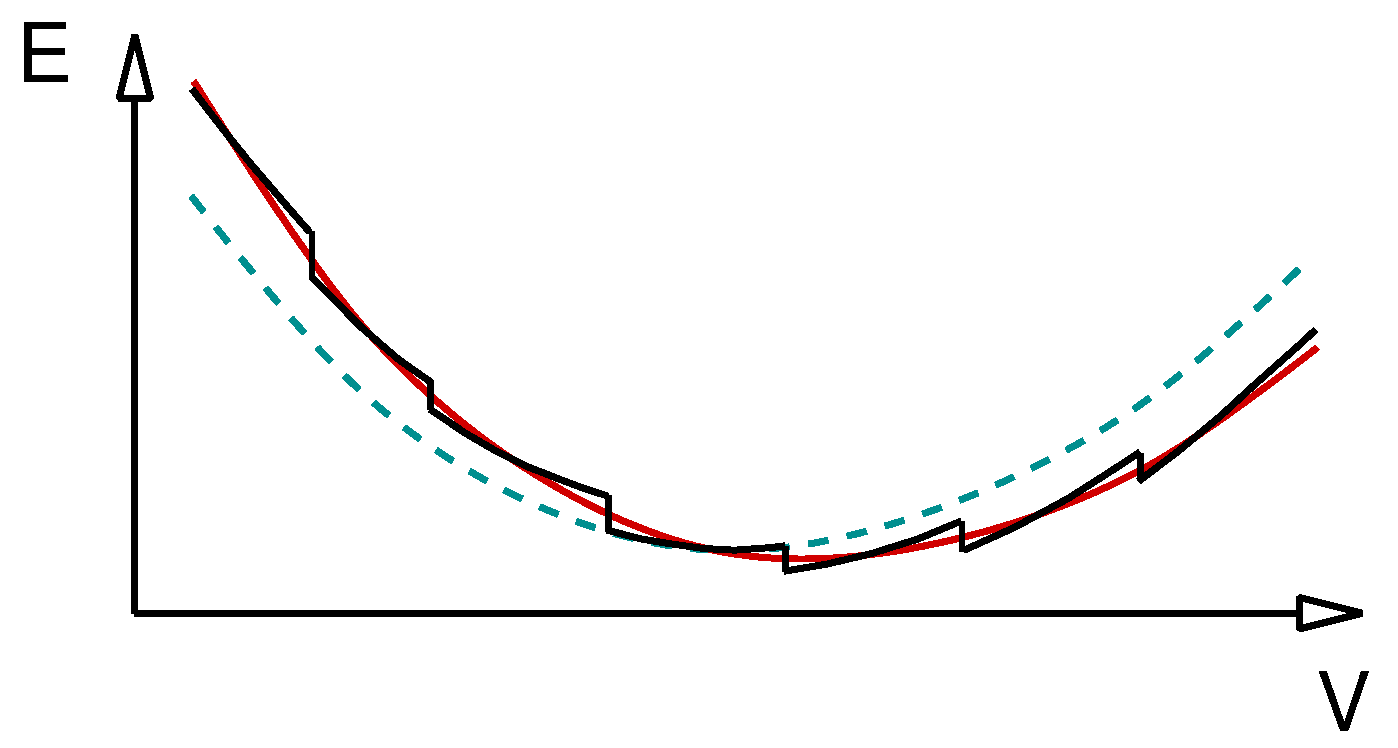
\includegraphics[width=6cm]{Figs/Sawtooth/sawtooth.eps}
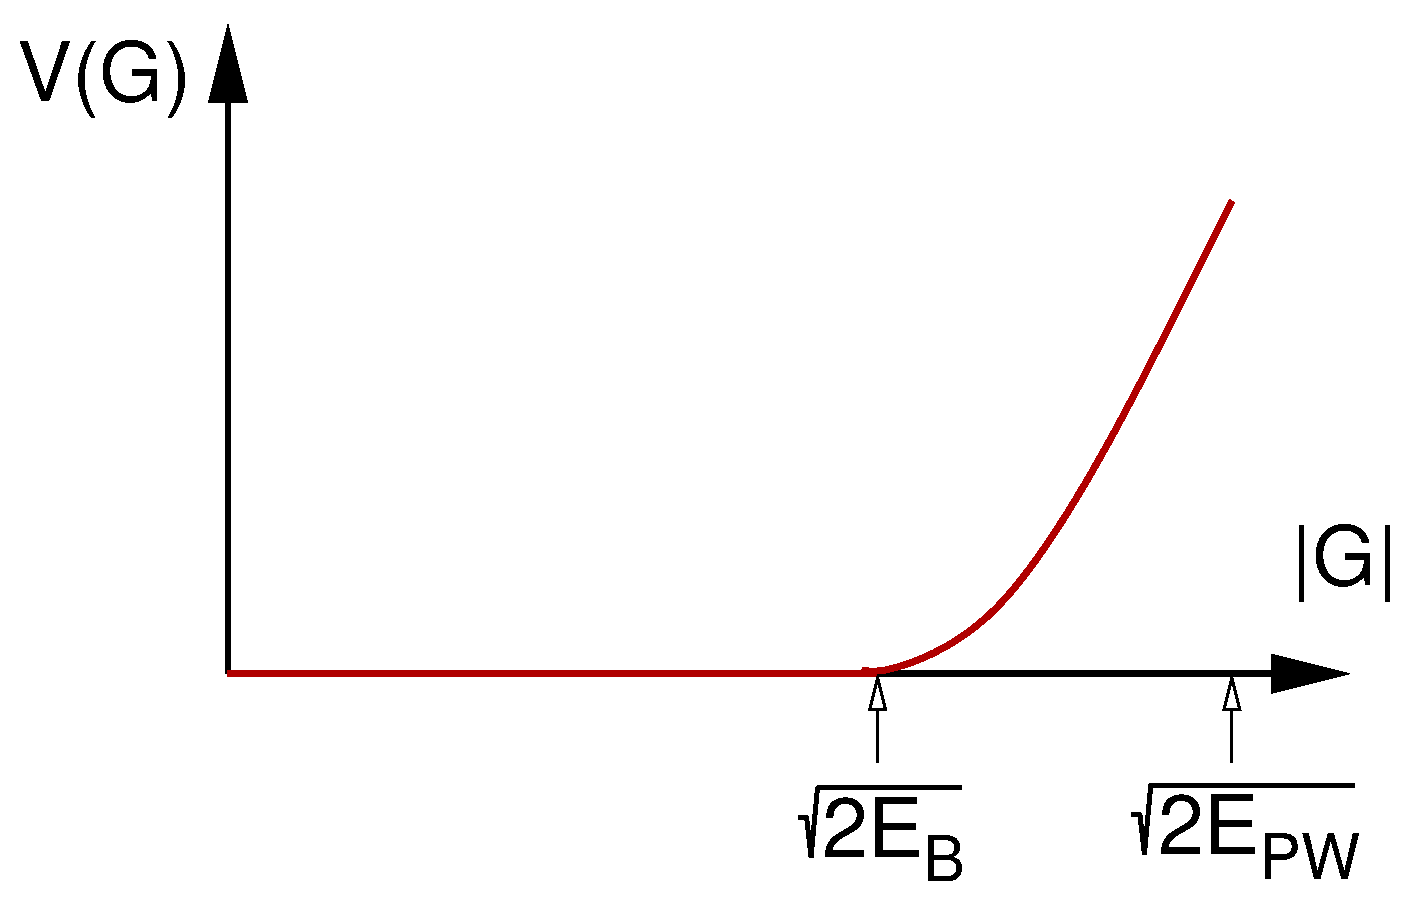
\includegraphics[width=6cm]{Figs/Gbucket/gbucket.eps}
\label{fig:sawtooth}
\caption{Left: Sawtooth behavior of the total energy as function of
volume with a fixed plane wave cutoff (black) with a fixed number of
plane waves (green dashed) and the correct result with a fully
converged calculation (red). By adding a G-dependent potential the
plane wave convergence can be artyificially accelerated.}
\end{figure}

The steps in the total energy vanish if the calculation is fully
converged in the basis set size, because additional basis functions do
not lower the total energy. If the function is not converged, the best
result is obtained by keeping the same plane wave cutoff. However, if
a the energy obtained at a few points is then fitted to a parabola or
the murnaghan equation of state, one has to be carefull with the
steps.

This sawtooth behavior can be suppressed by including an additional
G-dependent Bucket potential that ensures that the wave function
coefficients at the plane wave cutoff vanish strictly.




%==========================================================================
\subsection{Constraints acting on atoms}
%==========================================================================


%==========================================================================
\subsection{Electrostatic decoupling and coupling of point charges}
%==========================================================================


%}{} % end of \ifthenelse

%==========================================================================
\newpage
\section{Benchmarks}
%==========================================================================
Among the best calculations to compare energies are the calculations
using Numol by Becke\cite{Beckethermochemistry,DFTBenchmarks}.
Zero-point vibration energies have been tabulated by
Pople\cite{Pople}.


\section{Troubleshooting}

\subsection{Errors in the input data}

\begin{itemize}
\item A common mistake is to enter data with the wrong data type.
  In this case you will receive a message as follows, which should help
  to locate the problem.
\begin{verbatim}
TYPE INCONSISTENT
VARIABLE ID HAS THE VALUE DT
VARIABLE NTH HAS THE VALUE         1
VARIABLE TYPE EXPECTED HAS THE VALUE R(8)
VARIABLE ACTUAL TYPE HAS THE VALUE I(4)
STOP IN LINKEDLIST_GETGENERIC
\end{verbatim}
The first line says that there is a type mismatch. The last line
says that the problem happened in method of the linkedlist object,
which is also responsible for linked list/tree data structures such as
block-structured input files. In particular the program attempts to
collect a data item from this tree structure.  The second line gives
you the name of the variable, in this example ``DT'', which is the key
word for the time step. It cannot tell in which file or which block
the data is located. The third line tells you that it is the first
data with this name in the block. The next two lines say that the
program expects a data with type ``real(8)'', but finds one of type
``integer(4)''. It appears that the program has mistaken your data for
DT as an integer, because the user forgot to type the decimal point.
\item The program does not do what you want it to. You may have mistyped
  keywords, or mixed bup the tree structure. This renders a lot of data
  invisible, and the program uses the default values. Try to consult
  the protocol of the program. It should report all options selected.
  If options are not listed, the option is not selected, or the
  corresponding value is zero. (Of course, it can also be that it is
  not reported. In this case see whether you get a statement in the
  protocol if you select the option. If not, please report this to the
  author.)
\item If you did not provide, or mistype, a keyword that does not have
  a default, you may receive a message like this:
\begin{verbatim}
KEYWORD T= IS MANDATORY
STOP IN STRCIN; !STRUCTURE!LATTICE
\end{verbatim}

\end{itemize}
\subsubsection{Changes of Input data}

Here a list of syntactic changes for the input data. Although I am
trying to keep this list complete, please consult the description of
the input data to make sure.

\begin{enumerate}
\item !CONTROL!GENERIC:STOREPSIR \break$\rightarrow$ !CONTROL!PSIDYN:STOREPSIR
\item !CONTROL!PSIDYN:AUTO \break$\rightarrow$ !CONTROL!PSIDYN!AUTO
\item !CONTROL!RDYN:AUTO \break$\rightarrow$ !CONTROL!RDYN!AUTO
\item !CONTROL!FILES!FILE:IDENT \break$\rightarrow$ !CONTROL!FILES!FILE:ID
\item !STRUCTURE!GENERIC:NBAND \break$\rightarrow$ !STRUCTURE!OCCUPATIONS:NBAND
\item !STRUCTURE!GENERIC:NSPIN \break$\rightarrow$ !STRUCTURE!OCCUPATIONS:NSPIN
\item !STRUCTURE!GENERIC:CHARGE[-QEL]\break$\rightarrow$ !STRUCTURE!OCCUPATIONS:CHARGE[E]
\item !STRUCTURE!GENERIC:SPIN[-QEL] \break$\rightarrow$ !STRUCTURE!OCCUPATIONS:SPIN[HBAR]
\item !STRUCTURE!OCCUP \break$\rightarrow$ !STRUCTURE!OCCUPATIONS!STATE
\item !CNTL!PSIDYN:SAVEORTHO \break$\rightarrow$ !CNTL!PSIDYN:SAFEORTHO
\item !CNTL!ANALYSE!BOX disabled
\item !CONTROL!RNOSE \break$\rightarrow$ !CONTROL!RDYN!THERMOSTAT
\item !CONTROL!PSINOSE \break$\rightarrow$ !CONTROL!PSIDYN!THERMOSTAT
\end{enumerate}

\subsection{Runtime errors}

This is a list of nontrivial user errors from which the program is not
sufficiently protected and loose ends of the code where particular
caution is needed. It is my goal to adjust the program to
keep this list as short as possible.

\begin{enumerate}
\item Sometimes the program stops with an error message saying 
  ``LOOP FOR ORTHOGONALIZATION NOT CONVERGED''. This is an indication
  of extremely large changes of the wave functions, which can no
  longer be orthogonalized. There are several possible problems that can
  lead to this, and several possible remedies: 
  \begin{itemize}
  \item The atomic positions have been chosen with unreasonably short
    distances, or with atoms lying on top of each other.
  \item The number of valence electrons in the .strc file are not
    consistent with the setup files.
  \item Some setups produce this behavior in the first few time steps.
    In this case reduce the plane wave cutoff to a small value such as
    5, 10 or 20 Ry. If this alone does not help, also reduce the
    time step, but leave the masses constant. It is suffient to do
    this for the first few (about five or ten) time steps. If you
    started a new job with gradient corrected DFT functionals, you
    should try ``!CONTROL!FOURIER:CDUAL=4'' or reach convergence furst
    for a truly local functional before switching gradient corrections
    on. If the kinetic energy for the wave functions decreases to a
    reasonable value of a few Hartree, one can restart with the
    original values.
  \item If all this does not help, you are in trouble!
  \end{itemize}
\item{The number of valence electrons have not been chosen consistent with
    the atomic setup. The number of valence electrons for each atom is
    not printed in the protocol.}
\item If the program produces a coredump, increase first the stack size
  using the ``ulimit'' command. You can also control the size of the stack
  array using the compiler option -bmaxstack.
\item The code has a limited size of the send-receive buffer. The
  program is not guarded against a buffer overflow, even though the MPI
  Library should give a useful message (affects only the parallel
  version).
\item Errors occur if the operating system, Fortran runtime
  environment or SP2 Software are not on the same level, 
  used during compilation.
\item If you find that the program crashes without providing an error
  message, and if you have the source code, you can set
  ``TOFF=.false'' in the source file paw\_trace.f, and recompile. The
  program will then continuously write information on subroutines
  entered and left, which often allows one to locate the problem. Note that, in
  order to avoid producing files too large to be useful, not all
  routines result in a trace message.  \ifthenelse{\boolean{private}}{
\item The routine "MADELUNG" chooses itself the range of real and
    reciprocal space summations. It has not been sufficiently tested
    whether these choices are accurate. It may affect the result of
    the object "Isolate" that separates isolated molecules from its
    periodic images.
\item The Becke88 gradient correction for exchange produces
  unreasonable results if the total density or the spin density is
  vanishes. In this case small numerical values for the gradient pick
  up a singularity in the functional form. This may happen for a fully
  spin polarized system. The cure is to pick another density
  functional, which does not contain the Becke88 functional.
\item In the compiler xlf5.1.1 the code creates a segmentation fault
  in a parallel-synchonization routine. In that case an empirical
  solution is to reduce the optimization from O3 to O. There is no
  problem of this type in the scalar version.
}{} %end of ifthenelse
\end{enumerate}

%=========================================================
\subsection{Porting}
%=========================================================
\begin{itemize}
\item Your system may not have the Korn shell available. In that case
  change the first line of any shell scripts, namely {\tt \#!/bin/ksh}, to
    {\tt \#!/bin/bash}. Most shell scripts are in the main paw directory.
   There may be some commands that do not work with bash yet.
\item Adaptions of the preprocessor {\tt F90PP/f90pp}. (This is a self
  made preprocessor.
\item use the option {\bf -arch} when compiling the code with {\tt
    paw\_compile} to use settings for a compiler different from the
  IBM xlf compiler. To see if your compiler is included and what value
  to set use {\tt paw\_compile ?} to obtain the command line syntax.
\end{itemize}


\ifthenelse{\boolean{private}}{
%==========================================================================
\section{Suggestions}
%==========================================================================
\begin{itemize}
\item print the creation date of the executable. This could be done by
  small subroutine which simply prints the time. This subroutine is on
  a separate file paw\_date.f, which ``depends'' on the executable. A
  small shell script modifies paw\_date.f first by replacing a
  characteristic string by the current date and then compiles is. It
  is always compiled before the program is linked.
\item replace the covalent radii by the bond radii of UFF. give the
  reference in the manual.
\item make criterion for drawing bonds in the paw\_tra and the paw\_wave
  file user defineable. Instead of fixing it to 1.2 times the covalent
  radius, read the factor in.
\item check plotting eigenstates, versus wave functions
\item make selection for PDOS scaling in the paw\_dos tool
\item check if paw\_dos tool treats spin-polarized calculations properly
\end{itemize}
}{} % end of \ifthenelse

\newpage
%%==========================================================================
%\section{Literature}
%%==========================================================================
%%==========================================================================
%%\subsection{Introductory material}
%%==========================================================================
%\subsubsection{Electronic structure}
%\subsubsection{Molecular Dynamics}
%\subsubsection{Ab-initio Molecular Dynamics}
%\subsubsection{PAW Method}
%\subsubsection{Density functional Theory}
%%\begin{description}
%%\end{description}
%%==========================================================================
%\subsection{Recommended Literature}
%%==========================================================================
%\begin{description}
%\item[``Projector Augmented Wave method'', P.E. Bl\"ochl, Phys. Rev. B
%  {\bf 50}, 17953 (1994)] (Description of the PAW method)

%\item[W. Kohn and L. J. Sham, Phys. Rev. 140,A1133(1965)] Local
%  density approximation:

%\item[Perdew-Zunger, (Phys.Rev.B23, p5048(1981))] Parameterizations of
%  the exchange and correlation energy

%\item[J.P. Perdew, J. A. Chevary, S.H. Vosko, K.A. Jackson,
%  M.R. pederson, D.J. Singh and C. Fiolhais, Phys. Rev. B,
%  46,6671(1992-I)]
% Perdew-Wang gradient correction for correlation

%\item[J.P. Perdew, K. Burke and M. Ernzerhof,
%  Phys. Rev. Lett. submitted (1997)]
% Simplified version of Perdew Wang's 91 GGA-type exchange-correlation functional

%\item[K. Schwarz; Phys. Rev. B5, 2466 (1972)]X-alpha (alpha=0.7) 

%\item[Barth-Hedin (J.Phys.C5,p1629(1972))] 
%Parameterizations of the exchange and correlation energy,

%\item[??]Rajagopal-Singhal-Kimball \hfill\break 

%\item[J.Chem.Phys.96,p2155(1992)]Becke gradient correction

%\item[Phys. Rev. B33,p8822(1986))] Perdew gradient correction for
%  correlation

%\item[R. Car and M. Parrinello, Phys. Rev. Lett. 55, 2471 (1985)]
%  Original paper on first principles molecular dynamics

%\item[R. Car and M. Parrinello, in ``Simple molecular systems at very
%  high density''] ed. A Polian et al. (Plenum Publishing corporation,
%  1989) p455-476\hfill\break more extended description on ab-initio
%  MD. describes the method for orthogonalization in some detail

%\item[G. Pastore, E. Smargiassi and F. Buda, Phys. Rev. A 44, 6334
%  (1991)] detailed analysis of first principles MD

%\item[D.K. Kremler and P.A. Madden, Mol. Phys. 70, 921 (1990)] Review
%  article on first principles MD and the pseudopotential approach

%\item[J.-P. Ryckaert, G. Cicotti and H.J.C. Berendsen, J. Comp. Phys.
%  23.327 (1977)] original paper on treating constraints in a molecular
%  dynamics simulation

%\item[S. Nos\'e, J. Chem. Phys. 81, 511 (1984)] original paper on the
%  Nos\'e thermostat

%\item[S. Nos\'e, Mol. Phys. 52, 255 (1984)] paper on the Nos\'e thermostat

%\item[P.E.  Bl\"ochl and M. Parrinello, Phys. Rev. B. 45, 9413
%  (1992)]``Adiabaticity in first-principles molecular dynamics'', Nos\'e
%  thermostat for the electronic wave functions

%\item[]Mermin functional (finite temperature for the electrons,
%  variable occupations)

%\item[P.E. Bl\"ochl, Phys. Rev. {\bf B 41}, 5414 (1990)]''Generalized
%  separable pseudopotentials''. Precursor of the PAW method in the
%  pseudopotential formalism.

%\item[C.G. Van de Walle and P.E. Bl\"ochl, Phys. Rev. B {\bf 47} 4244
%  (1993)] Poor man's PAW applied to extract hyperfine parameters from
%  a pseudopotential calculation.

%\item[Peter E. Bl\"ochl, J. Chem. Phys. {\bf 103} 7422 (1995)]
%  ``Electrostatic decoupling of plane wave expanded densities
%  and  derived atomic point charges'',
%  Description of the isolate option to treat isolated molecules 
%\end{description}
% %==========================================================================
% \section{Applications of the PAW method (until June 1997)}
% %==========================================================================
% \begin{sloppypar}
% \begin{enumerate}
% \item ``Ab-initio calculations of one-dimensional band structures of
%   mixed-stack molecular crystals'', C. Katan, C. Koenig and P.E.
%   Bl\"ochl, Solid State Comm. 102, 589 (1997)
% %
% \item ``Ab-initio Molecular Dynamics Calculations to Study
%   Catalysis'', K. Schwarz, E. Nusterer, P. Margl and P.E. Bl\"ochl,
%   Int'l J. Quantum Chem. {\bf 61}, 369 (1997)
 
% \item ``A Static and Dynamic Density Functional Study of the Ti(IV)
%   Constrained Geometry Catalyst (CpSiH2NH)Ti-R+: 1. Resting States and
%   Chain Propagation'', Tom K. Woo, Peter Margl, John C.W. Lohrenz, Tom
%   Ziegler and Peter E. Bl\"ochl; J. Am. Chem.  Soc. {\bf 118}, 13021
%   (1996).
 
% \item ``First-Principles Investigation of Enantioselective Catalysis:
%   Asymmetric Allylic Amination with Pd Complexes Bearing P, N
%   Ligands'', P.E. Bl\"ochl and A. Togni, Organometallics {\bf 15},
%   4125 (1996).
  
% \item ``Interaction of Water and Methanol with a Zeolite at High
%   Coverages'', E. Nusterer, P.E. Bl\"ochl and K. Schwarz, Chem.  Phys.
%   Lett. {\bf 253}, 448 (1996)
  
% \item ``Migratory CO Insertion and Aldehyde Formation in Carbonylation
%   of Methane by the Rh(PH3)2Cl Catalyst. A Dynamical Density
%   Functional Study'', P. Margl, T. Ziegler and P.E.  Bl\"ochl, J. Am.
%   Chem. Soc. {\bf 118}, 5412 (1996)
  
% \item ``Ab-Initio Molecular Dynamics with the Projector Augmented Wave
%   Method'', P.E. Bl\"ochl, P. Margl und K. Schwarz, in {\it Chemical
%     Applications of Density Functional Methods}, B.B. Laird, R.B. Ross
%   and T. Ziegler (eds.)  (American Chemical Society, Washington D.C.,
%   1996), p.54
  
% \item ``Ab-Initio Molecular-Dynamics study of diffusion and defects in
%   Solid Li$_3$N'', J. Sarnthein, K. Schwarz and P.E. Bl\"ochl, Phys.
%   Rev. B {\bf 53}, 9084 (1996).
  
% \item ``A Dynamical Density Functional Study on the Reaction of
%   Ethylene with Cp$_2$Zr(C$_2$H$_5$)$^+$'', P. Margl, J.C. W Lohrenz,
%   T. Ziegler and P.E. Bl\"ochl, J. Am. Chem. Soc. {\bf 118}, 4434
%   (1996).
  
% \item ``First Principles Molecular Dynamics Simulations for Neutral
%   and Radical Anion of p-Chloranil''\hfill\break C. Katan, P.E.
%   Bl\"ochl, P. Margl and C. Koenig, Phys. Rev. B {\bf 53}, 12112
%   (1996).
      
% \item ``Structure and Dynamics of Methanol in a Zeolite'',
%   E.~Nusterer, P.E.~Bl\"ochl and K.~Schwarz, Angew. Chem.  Int'l Ed.
%   Engl.  {\bf 35}, 175 (1996); Angew. Chem. {\bf 108}, 187 (1996).
  
% \item ``Reaction of Methane with Rh(PH$_3$)$_2$Cl: A Dynamical Density
%   Functional Study'', P. Margl, T. Ziegler and P.E. Bl\"ochl, J. Am.
%   Chem. Soc {\bf 117}, 12625 (1995).
  
% \item ``Electronic Structure of Crystalline (NH$_4)_2$CuCl$_4$ from
%   First Principles, P. Carloni, P.E.~Bl\"ochl, P.L.~Orioli, Gazzetta
%   Chimica Italiana, {\bf 125} 497 (1995).
  
% \item "Electrostatic Decoupling of Periodic Images of
%   Plane-Wave-Expanded Densities and Derived Point Charges",
%   P.E.~Bl\"ochl, J. Chem. Phys. {\bf 103}, 7422 (1995).
  
% \item ``Dynamics of Beryllocene''\hfill\break P. Margl, K.  Schwarz
%   and P.E. Bl\"ochl, J. Chem. Phys. {\bf 103}, 683 (1995).
  
% \item ``The electronic structure of Cu, Zn superoxide dismutase active
%   site and its interactions with the substrate''\hfill\break P.
%   Carloni, P.E. Bl\"ochl and M. Parrinello, J. Phys. Chem. {\bf 99},
%   1338 (1995).
  
% \item ``Projector Augmented Wave Method''\hfill\break P.E. Bl\"ochl,
%   Phys. Rev. B {\bf 50}, 17953 (1994).
  
% \item ``Fluxional Dynamics of Beryllocene''\hfill\break P. Margl, K.
%   Schwarz and P.E. Bl\"ochl, J. Am. Chem. Soc. {\bf 116}, 11177 (1994).
      
% \item ``Finite Temperature Characterization of Ferrocene from
%   First-Principles Molecular Dynamics Simulations''\hfill\break P.
%   Margl, K. Schwarz and P.E. Bl\"ochl, J. Chem. Phys. {\bf 100}, 8617
%   (1994).
  
% \item ``Adsorption and STM imaging of organic molecules from first
%   principles'',\hfill\break A.J. Fisher and P. Bl\"ochl, in {\it
%     Computations for the Nano-Scale} ed. P.E. Bl\"ochl, C.Joachim and
%   A.J. Fisher (Kluwer Academic Publishers, Dordrecht, 1993) 185.
  
% \item ``First-principles calculations of organometallic
%   compounds''\hfill\break P. Margl, K. Schwarz and P. E. Bl\"ochl, in
%   {\bf Computations for the Nano-Scale} ed. P.E. Bl\"ochl, C.Joachim
%   and A.J.~Fisher (Kluwer Academic Publishers, Dordrecht, 1993)
%   153-162.

% \item ``Adsorption and scanning-tunneling microscope imaging of benzene
%   on graphite and MoS$_2$''\hfill\break A.J. Fisher and P. Bl\"ochl,
%   Phys. Rev. Lett. {\bf 70}, 3263 (1993).

% \item ``Hypothetical carbon modifications derived from zeolite
%   frameworks''\hfill\break R. Nesper, K. Vogel and P.E. Bl\"ochl, Angew.
%   Chem. Int. Ed. Engl. {\bf 32}, 701 (1993).

% \item ``Hypothetische Kohlenstoffmodifikationen mit Zeolith-analogen
%   Strukturen''\hfill\break R. Nesper, K. Vogel and P.E. Bl\"ochl, Angew.
%   Chem. {\bf 105}, 786 (1993).
% %25
% \item C.G.~Van~de~Walle and P.E.~Bl\"ochl, Phys. Rev. B
%   {\bf 47} 4244 (1993).
% %??
% \item``Generalized separable pseudopotentials''
%   P.E.~Bl\"ochl, Phys. Rev. {\bf B 41}, 5414 (1990).
% \end{enumerate}
% \end{sloppypar}


%====================================================================
\newpage
\begin{thebibliography}{99}
%0
\bibitem{Pdcat} ``First-Principles Investigation of Enantioselective
  Catalysis: Asymmetric Allylic Amination with Pd Complexes Bearing P,
  N Ligands'', P.E. Bl\"ochl and A. Togni, Organometallics {\bf 15},
  4125 (1996).
%1
\bibitem{PAW}``Projector Augmented Wave Method'', P.E. Bl\"ochl, Phys.
  Rev. B {\bf 50}, 17953 (1994).
%2
\bibitem{KohnSham} ``Inhomogeneous Electron Gas'', P.~Hohenberg and
  W.~Kohn, Phys. Rev.{\bf 136} B 864 (1964); ``Selfconsistent Equations
  including exchange and Correlation Effects'', W.~Kohn and L.J.~Sham,
  Phys. Rev. {\bf 140}, A1133 (1965)
%3
\bibitem{DFTBenchmarks} ``Density Functional Thermochemistry~II. The
  effect of the Perdew-Wang Generalized-Gradient Correlation
  Correction'', A.D.~Becke, J. Chem. Phys. {\bf 97}, 9173 (1992),
  ``Basis-set-free local density-functional calculations of geometries
  of polyatiomic molecules'', R.M.~Dickson and A.D.~Becke,
  J. Chem. Phys. {\bf 99}, 3898 (1993).
%4
\bibitem{CP}``Unified Approach for Molecular Dynamics and Density
  Functional Theory'', R.~Car and M.~Parrinello, Phys. Rev. Lett. {\bf
    55}, 2471 (1985).
%5
\bibitem{CP2} ``The Unified Approach for Molecular Dynamics and
  Density Functional Theory'', R. Car and M. Parrinello, in {\it
    Simple molecular systems at very high density} ed. A. Polian et
  al. (Plenum, New York, 1989) p455-476.
%6
\bibitem{Pastore}G.~Pastore, E.~Smargiassi and F.~Buda, Phys. Rev. A
  {\bf 44}, 6334 (1991).
%7
\bibitem{Madden} ``Molecular Dynamics without Effective Potentials via
  the Car-Parrinello Approach'', D.K.~Kremler and P.A.~Madden, Mol.
  Phys. {\bf 70}, 921 (1990).
%8
\bibitem{Decouple}``Electrostatic decoupling of plane wave expanded
  densities and derived atomic point charges'', P.E.~Bl\"ochl, J.
  Chem. Phys. {\bf 103}, 7422 (1995).
%9
\bibitem{MPI} Message Passing Interface. Software for interprocessor
  communication on parallel computers. See
  ``http://www.osc.edu/Lam/lam.html\#MPI'' for more information.
%10
\bibitem{ESSL} Engineering and Scientific Subroutine Library is a
  product of IBM. See
  ``http://direct.boulder.ibm.com/rsdirect/us/software/essl.htm'' for
  more information.
%
\bibitem{grimme04_jcc25_1463}S. Grimme, \textit{Accurate description
of Van der Waals complexes by density functional theory including
empirical corrections}, J. Comput. Chem. \textbf{25},1463 (2004).
%0
\bibitem{IRC} ``A Formulation of the Reaction Coordinate'' J. Phys.
  Chem. {\bf 74}, 4161 (1970); ``The Path of Chemical Reactions -- The
  IRC Approach'' Acc. Chem. Res. {\bf 14}, 363 (1981).
%11
\bibitem{Constants}``The Fundamental Physical Constants'' E.R.~Cohen
  and B.N. Taylor, Physics Today {\bf 49} (Buyers Guide), 9 (1996) and
  references therein.
%12
\bibitem{Dataexplorer} The IBM Visualization Dataexplorer is a
  general-purpose software package for data visualization and
  analysis. See ``http://www.opendx.org/'' for information. It is now
  an open source project and publically available at no cost.
%13
\bibitem{XMGR}XMGR is an XY plotting tool written by 
  Paul~J.~Turner. The development is currently being continued by a group of
  volunteers.  For information on how to obtain access, see
  ``http://plasma-gate.weizmann.ac.il/Xmgr/''.
%14
\bibitem{Cerius2} Cerius$^2$ is a product of Molecular Simulations
  Inc. See ``http://www.msi.com/info/products/Cerius2.html'' for more
  information.
%15
\bibitem{PerdewZunger} ``Self-interaction correction to
  density-functional approximations for many-electron
  systems'', J.P.~Perdew and A.~Zunger, Phys. Rev. B {\bf 23}, 5048 (1981).
%16
\bibitem{CeperleyAlder} ``Ground State of the Electron Gas by a
  Stochastic Method'' D.M.~Ceperley and B.J.~Alder, Phys. Rev.
  Lett. {\bf 45}, 566 (1980).
%17
\bibitem{GGA91}``Atoms, Molecules, Solids, and Surfaces: Applications
  of the Generalized Gradient Approximation for Exchange and
  Correlation'', J.P.~Perdew, J. A. Chevary, S.H.~Vosko, K.A.~Jackson,
  M.R.~Pederson, D.J.~Singh and C.~Fiolhais, Phys. Rev. B, {\bf 46},
  6671 (1992-I).
%17
\bibitem{PW91L} ``Accurate and simple analytic representation of the
  electron gas correlation energy'', J.P.~Perdew and Y.~Wang,
  Phys. Rev.B {\bf 45}, 13244 (1992-I)
%18
\bibitem{Becke88}``Density Functional Exchange Energy Approxiamtion
  with Correct Asymptotic Behavior'', A.D.~Becke, J. Chem. Phys.{\bf
    96}, 2155 (1992).
%19
\bibitem{Perdew86} ``Density-Functional Approximations for the
  Correlation Energy of the Inhomogeneous Electron Gas'', J.P.~Perdew,
  Phys. Rev. B {\bf 33}, 8822 (1986)).
%20
\bibitem{PBE}``Generalized Gradient Approximation Made Simple'',
  J.P.~Perdew, K.~Burke and M.~Ernzerhof, Phys. Rev. Lett. {\bf 77},
  3865 (1996).
%20
\bibitem{RPBE}``Improved Adsorption Energies within Density-Functional Theory 
       using Revised Perdew-Burke-Ernzerhof Functionals'',
  B. Hammer, L.B. Hansen, and J.K. Norskov, Phys. Rev. B {\bf 59},
  7413 (1999).
%21
\bibitem{Verlet}``Practical Algorithms for Dynamic Simulations'',
  H.J.C.~Berendsen and W.F.~van Gunsteren, Varenna Notes (1985), p43.
%22
\bibitem{Acceleration}``Acceleration schemes for ab-initio molecular
  dynamics simulations and electronic structure calculations''
  F.~Tassone, F.~Mauri and R.~Car, Phys. Rev. B {\bf 50}, 10561
  (1994-I)
%23
\bibitem{Adiabaticity}``Adiabaticity in first-principles molecular
  dynamics'', P.E.~Bl\"ochl and M.~Parrinello, Phys. Rev. B {\bf 45},
  9413 (1992).
%24
\bibitem{Nose}``A unified formulation of the constant temperature
  molecular dynamics methods'', S.~Nos\'e, J. Chem. Phys. {\bf 81}, 511
  (1984); ``A molecular dynamics method for simulation in the
  canonical ensemble'', S.~Nos\'e, Mol.  Phys. {\bf 52}, 255 (1984),
  ``Canonical Dynamics: Equilibrium phase-space distributions'', W.G.
  Hoover, Phys. Rev. A {\bf 31}, 1695 (1985).
%25
\bibitem{Constraints} ``Numerical Integration of the Cartesian
  Equations of Motion of Systems with Constraints: Molecular
  Dynamics of n-Alkanes'' J.-P.~Ryckaert, G.~Cicotti and H.J.C.~Berendsen,
  J. Comp. Phys. {\bf 23}, 327 (1977).
%26
\bibitem{HinSi} ``First-Principles Calculations of Diffusion Constants:
  Hydrogen in Silicon'', P.E.~Bl\"ochl, C.G.~Van~de~Walle and
  S.T.~Pantelides, Phys. Rev. Lett. {\bf 64}, 1401 (1990). 
%27
\bibitem{UFF} ``UFF, a fully periodic table force field for molecular
  mechanics and molecular dynamics simulations'' A.K.~Rappe,
  C.J.~Casewit, K.S.~Colwell, W.A.~Goddard~III, and W.M.~Skiff,
  J. Am. Chem. Soc. {\bf 114}, 10024 (1992).
%28
\bibitem{FreeSoftwareFoundation} For information of software from the
  free software foundation, see ``http://www.gnu.ai.mit.edu/''
%??
\bibitem{LDA+U}``Band Theory and Mott Insulators: Hubbard U instead of
  Stoner I'', V.I.~Anisimov, J.~Zaanen and 
O.K.~Andersen, Phys. Rev. B {\bf 44}, 943 (1991).
%
\bibitem{MPEGPLAY}``http://www.geom.umn.edu/software/mpeg\_play/''
%
\bibitem{MPEGENCODE} ``http://www.imag.fr/Multimedia/archives/unix.html''
%
\bibitem{Beckethermochemistry}``Density Functional Thermochemistry I:
  The effect of exchange-only gradient correction'', A.D. Becke,
  J.chem. Phys. {\bf 96}, 2155 (1992); ``Density Functional
  Thermochemistry II: The effect of Perdew Wang generalized-gradient
  correlation correction'', A.D. Becke, J.chem. Phys. {\bf 97}, 9173
  (1992);
%
\bibitem{Pople} ``Gaussian-1 theory: A general procedure for prediction
  of molecular energies'' J.A. Pople, M. Head-Gordon and D.J. Fox,
  J. Chem. Phys. {\bf 90}, 5622 (1989); ``Gaussian-1 theory of
  molecular energies for second-row compounds'' L.A. Curtiss,
  C. Jones, G.W. trucks and K. Raghavachari,
  J. Chem. Phys. {\bf 93}, 2537(1990)
\end{thebibliography}
\printindex
\end{document}
\bye
%====================================================================
